\documentclass[a4paper,12pt]{report}
\usepackage[left=2cm,right=2cm,top=2cm,bottom=3cm]{geometry}

%stuff I've added
\usepackage[utf8]{inputenc}
\usepackage{graphicx}% Include figure files
% \usepackage{dcolumn}% Align table columns on decimal point
% \usepackage{bm}% bold math
\usepackage{acronym}
\usepackage{physics}
% \usepackage{layouts}
\usepackage{acronym}
\usepackage{lipsum} 

\usepackage{amsmath}
\usepackage{amssymb}
\usepackage{svg}
\usepackage{comment}
\usepackage{placeins}
\usepackage{float}
\floatplacement{figure}{H} % the default figure placement specifier

\usepackage{hyperref}
\usepackage{cleveref}
\usepackage{bookmark}

\usepackage{pdfpages} % To be able to include pdfs in the appendix

\usepackage[version=4]{mhchem} % for chemical formulas

\usepackage[style=numeric,
sorting=none,
hyperref=true]{biblatex}
\addbibresource{entire_zotero_library.bib}

% \def\[#1\]{\begin{equation}#1\end{equation}}

% Exrta symbol commands
\newcommand{\tex}[1]{\expval{#1}} %Thermal expectation value
\newcommand{\qex}[1]{\expval{#1}} %Quantum expectation value
\newcommand{\Z}{\mathcal{Z}} %Partition function
\newcommand{\T}{\mathcal{T}} %MCMC Transition function
\newcommand{\A}{\mathcal{A}} %MCMC Acceptance function
\newcommand{\p}{\mathcal{P}} %MCMC Proposal distribution
\newcommand{\nfi}{n^f_i} %FK number operators of f electrons
\newcommand{\nfj}{n^f_j} %FK number operators of f electrons
\newcommand{\s}{\vec{s}} %used to refer to states of the spin system

\usepackage{orcidlink}

%for code blocks
\usepackage{listings}
\usepackage{xcolor}

\definecolor{codegreen}{rgb}{0,0.6,0}
\definecolor{codegray}{rgb}{0.5,0.5,0.5}
\definecolor{codepurple}{rgb}{0.58,0,0.82}
\definecolor{backcolour}{rgb}{0.95,0.95,0.92}
\definecolor{urlblue}{HTML}{007bff}

\lstdefinestyle{mystyle}{
    backgroundcolor=\color{backcolour},   
    commentstyle=\color{codegreen},
    keywordstyle=\color{magenta},
    numberstyle=\tiny\color{codegray},
    stringstyle=\color{codepurple},
    basicstyle=\ttfamily\footnotesize,
    breakatwhitespace=false,         
    breaklines=true,                 
    captionpos=b,                    
    keepspaces=true,                 
    numbers=left,                    
    numbersep=5pt,                  
    showspaces=false,                
    showstringspaces=false,
    showtabs=false,                  
    tabsize=2
}

\lstset{style=mystyle}
%endfor code blocks

% \begin{acronym}
    \newacro{FK}{Falikov-Kimball}
    \newacro{CDW}[CDW]{charge-density wave}
    \newacro{MCMC}{Markov chain Monte Carlo}
    \newacro{ED}{Exact Diagonalisation}
    \newacro{TMM}{Transfer Matrix Methods}
    \newacro{IPR}{Inverse Participation Ratio}
    \newacro{DOS}{density of states}
    \newacro{FTPT}{finite temperature phase transition}
    \newacro{LRI}{Long-Range Ising}
% \end{acronym}

\hypersetup{
    colorlinks = true,
    linkcolor  = black,
    citecolor  = black,
    urlcolor   = urlblue,
}

\urlstyle{same}

\usepackage{wrapfig}
\usepackage{floatflt}

%stuff that came in the template

\usepackage{graphicx}
\usepackage{verbatim}
\usepackage{latexsym}
\usepackage{mathchars}
\usepackage{setspace}

\setlength{\parskip}{\medskipamount}  % a little space before a \par
\setlength{\parindent}{0pt}	      % don't indent first lines of paragraphs
%UHEAD.STY  If this is included after \documentstyle{report}, it adds
% an underlined heading style to the LaTeX report style.
% \pagestyle{uheadings} will put underlined headings at the top
% of each page. The right page headings are the Chapter titles and
% the left page titles are supplied by \def\lefthead{text}.

% Ted Shapin, Dec. 17, 1986

\makeatletter
\def\chapapp2{Chapter}

\def\appendix{\par
 \setcounter{chapter}{0}
 \setcounter{section}{0}
 \def\chapapp2{Appendix}
 \def\@chapapp{Appendix}
 \def\thechapter{\Alph{chapter}}}

\def\ps@uheadings{\let\@mkboth\markboth
% modifications
\def\@oddhead{\protect\underline{\protect\makebox[\textwidth][l]
		{\sl\rightmark\hfill\rm\thepage}}}
\def\@oddfoot{}
\def\@evenfoot{}
\def\@evenhead{\protect\underline{\protect\makebox[\textwidth][l]
		{\rm\thepage\hfill\sl\leftmark}}}
% end of modifications
\def\chaptermark##1{\markboth {\ifnum \c@secnumdepth >\m@ne
 \chapapp2\ \thechapter. \ \fi ##1}{}}%
\def\sectionmark##1{\markright {\ifnum \c@secnumdepth >\z@
   \thesection. \ \fi ##1}}}
\makeatother
%%From: marcel@cs.caltech.edu (Marcel van der Goot)
%%Newsgroups: comp.text.tex
%%Subject: illegal modification of boxit.sty
%%Date: 28 Feb 92 01:10:02 GMT
%%Organization: California Institute of Technology (CS dept)
%%Nntp-Posting-Host: andromeda.cs.caltech.edu
%%
%%
%%Quite some time ago I posted a file boxit.sty; maybe it made it
%%to some archives, although I don't recall submitting it. It defines
%%	\begin{boxit}
%%	...
%%	\end{boxit}
%%to draw a box around `...', where the `...' can contain other
%%environments (e.g., a verbatim environment). Unfortunately, it had
%%a problem: it did not work if you used it in paragraph mode, i.e., it
%%only worked if there was an empty line in front of \begin{boxit}.
%%Luckily, that is easily corrected.
%%
%%HOWEVER, apparently someone noticed the problem, tried to correct it,
%%and then distributed this modified version. That would be fine with me,
%%except that:
%%1. There was no note in the file about this modification, it only has my
%%   name in it.
%%2. The modification is wrong: now it only works if there is *no* empty
%%   line in front of \begin{boxit}. In my opinion this bug is worse than
%%   the original one.
%%
%%In particular, the author of this modification tried to force an empty
%%line by inserting a `\\' in the definition of \Beginboxit. If you have
%%a version of boxit.sty with a `\\', please delete it. If you have my
%%old version of boxit.sty, please also delete it. Below is an improved
%%version.
%%
%%Thanks to Joe Armstrong for drawing my attention to the bug and to the
%%illegal version.
%%
%%                                          Marcel van der Goot
%% .---------------------------------------------------------------
%% | Blauw de viooltjes,                    marcel@cs.caltech.edu
%% |    Rood zijn de rozen;
%% | Een rijm kan gezet
%% |    Met plaksel en dozen.
%% |


% boxit.sty
% version: 27 Feb 1992
%
% Defines a boxit environment, which draws lines around its contents.
% Usage:
%   \begin{boxit}
%	... (text you want to be boxed, can contain other environments)
%   \end{boxit}
%
% The width of the box is the width of the contents.
% The boxit* environment behaves the same, except that the box will be
% at least as wide as a normal paragraph.
%
% The reason for writing it this way (rather than with the \boxit#1 macro
% from the TeXbook), is that now you can box verbatim text, as in
%   \begin{boxit}
%   \begin{verbatim}
%   this better come out in boxed verbatim mode ...
%   \end{verbatim}
%   \end{boxit}
%
%						Marcel van der Goot
%						marcel@cs.caltech.edu
%

\def\Beginboxit
   {\par
    \vbox\bgroup
	   \hrule
	   \hbox\bgroup
		  \vrule \kern1.2pt %
		  \vbox\bgroup\kern1.2pt
   }

\def\Endboxit{%
			      \kern1.2pt
		       \egroup
		  \kern1.2pt\vrule
		\egroup
	   \hrule
	 \egroup
   }	

\newenvironment{boxit}{\Beginboxit}{\Endboxit}
\newenvironment{boxit*}{\Beginboxit\hbox to\hsize{}}{\Endboxit}
\pagestyle{empty}

%

\makeatletter  %to avoid error messages generated by "\@". Makes Latex treat "@" like a letter

% \linespread{1.5} % enable to go back to 1.5 line spacing
\def\submitdate#1{\gdef\@submitdate{#1}}

\def\maketitle{
  \begin{titlepage}{
    %\linespread{1.5}
    \Large Imperial College of Science, Technology and Medicine \\
    %\linebreak
    Department of Physics
    \rm
    \vskip 3in
    \Large \bf \@title \par
  }
  \vskip 0.3in
  \par
  {\Large \@author}
  \vskip 4in
  \par
  Submitted in part fulfilment of the requirements for the degree of 
  \linebreak
  Doctor of Philosophy in Physics of Imperial College of Science, Technology and Medicine \@submitdate
  \vfil
  \end{titlepage}
}

\def\titlepage{
  \newpage
  \centering
  \linespread{1}
  \normalsize
  \vbox to \vsize\bgroup\vbox to 9in\bgroup
}
\def\endtitlepage{
  \par
  \kern 0pt
  \egroup
  \vss
  \egroup
  \cleardoublepage
}

\def\abstract{
  \pagenumbering{arabic}
  \begin{center}{
    \large\bf Abstract}
  \end{center}
  \small
  %\def\baselinestretch{1.5}
  % \linespread{1.5}
  \normalsize
}
\def\endabstract{
  \par
}

\newenvironment{acknowledgements}{
  \cleardoublepage
  \begin{center}{
    \large \bf Acknowledgements}
  \end{center}
  \small
  % \linespread{1.5}
  \normalsize
}{\cleardoublepage}
\def\endacknowledgements{
  \par
}

\newenvironment{dedication}{
  \cleardoublepage
  \begin{center}{
    \large \bf Dedication}
  \end{center}
  \small
  % \linespread{1.5}
  \normalsize
}{\cleardoublepage}
\def\enddedication{
  \par
}

\def\preface{
    % \pagenumbering{roman}
    \pagestyle{plain}
    % \doublespacing
}

\def\body{
    \pagestyle{plain}
    \cleardoublepage    
    \setlength{\parskip}{1.1ex}
    \tableofcontents
    % \cleardoublepage
    % \pagestyle{uheadings}
    % \listoftables
    % \pagestyle{plain}
    % \cleardoublepage

    \listoffigures
    \cleardoublepage

    \pagestyle{fancy}
    \setlength{\parskip}{2ex plus 0.5ex minus 0.2ex}
    \setlength{\parindent}{0pt}
}

\makeatother  %to avoid error messages generated by "\@". Makes Latex treat "@" like a letter

\newcommand{\ipc}{{\sf ipc}}

\newcommand{\Prob}{\bbbp}
\newcommand{\Real}{\bbbr}
% \newcommand{\real}{\Real}
\newcommand{\Int}{\bbbz}
\newcommand{\Nat}{\bbbn}

\newcommand{\NN}{{\sf I\kern-0.14emN}}   % Natural numbers
\newcommand{\ZZ}{{\sf Z\kern-0.45emZ}}   % Integers
\newcommand{\QQQ}{{\sf C\kern-0.48emQ}}   % Rational numbers
\newcommand{\RR}{{\sf I\kern-0.14emR}}   % Real numbers
\newcommand{\KK}{{\cal K}}
\newcommand{\OO}{{\cal O}}
\newcommand{\AAA}{{\bf A}}
\newcommand{\HH}{{\bf H}}
\newcommand{\II}{{\bf I}}
\newcommand{\LL}{{\bf L}}
\newcommand{\PP}{{\bf P}}
\newcommand{\PPprime}{{\bf P'}}
\newcommand{\QQ}{{\bf Q}}
\newcommand{\UU}{{\bf U}}
\newcommand{\UUprime}{{\bf U'}}
\newcommand{\zzero}{{\bf 0}}
\newcommand{\ppi}{\mbox{\boldmath $\pi$}}
\newcommand{\aalph}{\mbox{\boldmath $\alpha$}}
\newcommand{\bb}{{\bf b}}
\newcommand{\ee}{{\bf e}}
\newcommand{\mmu}{\mbox{\boldmath $\mu$}}
\newcommand{\vv}{{\bf v}}
\newcommand{\xx}{{\bf x}}
\newcommand{\yy}{{\bf y}}
\newcommand{\zz}{{\bf z}}
\newcommand{\oomeg}{\mbox{\boldmath $\omega$}}
\newcommand{\res}{{\bf res}}
\newcommand{\cchi}{{\mbox{\raisebox{.4ex}{$\chi$}}}}
%\newcommand{\cchi}{{\cal X}}
%\newcommand{\cchi}{\mbox{\Large $\chi$}}

% Logical operators and symbols
\newcommand{\imply}{\Rightarrow}
\newcommand{\bimply}{\Leftrightarrow}
\newcommand{\union}{\cup}
\newcommand{\intersect}{\cap}
\newcommand{\boolor}{\vee}
\newcommand{\booland}{\wedge}
\newcommand{\boolimply}{\imply}
\newcommand{\boolbimply}{\bimply}
\newcommand{\boolnot}{\neg}
\newcommand{\boolsat}{\!\models}
\newcommand{\boolnsat}{\!\not\models}


% \newcommand{\op}[1]{\mathrm{#1}}
% \newcommand{\s}[1]{\ensuremath{\mathcal #1}}

% Properly styled differentiation and integration operators
\newcommand{\diff}[1]{\mathrm{\frac{d}{d\mathit{#1}}}}
\newcommand{\diffII}[1]{\mathrm{\frac{d^2}{d\mathit{#1}^2}}}
\newcommand{\intg}[4]{\int_{#3}^{#4} #1 \, \mathrm{d}#2}
\newcommand{\intgd}[4]{\int\!\!\!\!\int_{#4} #1 \, \mathrm{d}#2 \, \mathrm{d}#3}

% Large () brackets on different lines of an eqnarray environment
\newcommand{\Leftbrace}[1]{\left(\raisebox{0mm}[#1][#1]{}\right.}
\newcommand{\Rightbrace}[1]{\left.\raisebox{0mm}[#1][#1]{}\right)}

% Funky symobols for footnotes
\newcommand{\symbolfootnote}{\renewcommand{\thefootnote}{\fnsymbol{footnote}}}
% now add \symbolfootnote to the beginning of the document...

\newcommand{\normallinespacing}{\renewcommand{\baselinestretch}{1.5} \normalsize}
\newcommand{\mediumlinespacing}{\renewcommand{\baselinestretch}{1.2} \normalsize}
\newcommand{\narrowlinespacing}{\renewcommand{\baselinestretch}{1.0} \normalsize}
\newcommand{\bump}{\noalign{\vspace*{\doublerulesep}}}
\newcommand{\cell}{\multicolumn{1}{}{}}
\newcommand{\spann}{\mbox{span}}
\newcommand{\diagg}{\mbox{diag}}
\newcommand{\modd}{\mbox{mod}}
\newcommand{\minn}{\mbox{min}}
\newcommand{\andd}{\mbox{and}}
\newcommand{\forr}{\mbox{for}}
\newcommand{\EE}{\mbox{E}}

\newcommand{\deff}{\stackrel{\mathrm{def}}{=}}
\newcommand{\syncc}{~\stackrel{\textstyle \rhd\kern-0.57em\lhd}{\scriptstyle L}~}

\def\coop{\mbox{\large $\rhd\!\!\!\lhd$}}
\newcommand{\sync}[1]{\raisebox{-1.0ex}{$\;\stackrel{\coop}{\scriptscriptstyle
#1}\,$}}

\newtheorem{definition}{Definition}[chapter]
\newtheorem{theorem}{Theorem}[chapter]

%%% For things that pandoc uses
\newenvironment{Shaded}{}{}
\newenvironment{Highlighting}{}{}
\newcommand{\AlertTok}[1]{\textcolor[rgb]{1.00,0.00,0.00}{\textbf{#1}}}
\newcommand{\AnnotationTok}[1]{\textcolor[rgb]{0.38,0.63,0.69}{\textbf{\textit{#1}}}}
\newcommand{\AttributeTok}[1]{\textcolor[rgb]{0.49,0.56,0.16}{#1}}
\newcommand{\BaseNTok}[1]{\textcolor[rgb]{0.25,0.63,0.44}{#1}}
\newcommand{\BuiltInTok}[1]{#1}
\newcommand{\CharTok}[1]{\textcolor[rgb]{0.25,0.44,0.63}{#1}}
\newcommand{\CommentTok}[1]{\textcolor[rgb]{0.38,0.63,0.69}{\textit{#1}}}
\newcommand{\CommentVarTok}[1]{\textcolor[rgb]{0.38,0.63,0.69}{\textbf{\textit{#1}}}}
\newcommand{\ConstantTok}[1]{\textcolor[rgb]{0.53,0.00,0.00}{#1}}
\newcommand{\ControlFlowTok}[1]{\textcolor[rgb]{0.00,0.44,0.13}{\textbf{#1}}}
\newcommand{\DataTypeTok}[1]{\textcolor[rgb]{0.56,0.13,0.00}{#1}}
\newcommand{\DecValTok}[1]{\textcolor[rgb]{0.25,0.63,0.44}{#1}}
\newcommand{\DocumentationTok}[1]{\textcolor[rgb]{0.73,0.13,0.13}{\textit{#1}}}
\newcommand{\ErrorTok}[1]{\textcolor[rgb]{1.00,0.00,0.00}{\textbf{#1}}}
\newcommand{\ExtensionTok}[1]{#1}
\newcommand{\FloatTok}[1]{\textcolor[rgb]{0.25,0.63,0.44}{#1}}
\newcommand{\FunctionTok}[1]{\textcolor[rgb]{0.02,0.16,0.49}{#1}}
\newcommand{\ImportTok}[1]{#1}
\newcommand{\InformationTok}[1]{\textcolor[rgb]{0.38,0.63,0.69}{\textbf{\textit{#1}}}}
\newcommand{\KeywordTok}[1]{\textcolor[rgb]{0.00,0.44,0.13}{\textbf{#1}}}
\newcommand{\NormalTok}[1]{#1}
\newcommand{\OperatorTok}[1]{\textcolor[rgb]{0.40,0.40,0.40}{#1}}
\newcommand{\OtherTok}[1]{\textcolor[rgb]{0.00,0.44,0.13}{#1}}
\newcommand{\PreprocessorTok}[1]{\textcolor[rgb]{0.74,0.48,0.00}{#1}}
\newcommand{\RegionMarkerTok}[1]{#1}
\newcommand{\SpecialCharTok}[1]{\textcolor[rgb]{0.25,0.44,0.63}{#1}}
\newcommand{\SpecialStringTok}[1]{\textcolor[rgb]{0.73,0.40,0.53}{#1}}
\newcommand{\StringTok}[1]{\textcolor[rgb]{0.25,0.44,0.63}{#1}}
\newcommand{\VariableTok}[1]{\textcolor[rgb]{0.10,0.09,0.49}{#1}}
\newcommand{\VerbatimStringTok}[1]{\textcolor[rgb]{0.25,0.44,0.63}{#1}}
\newcommand{\WarningTok}[1]{\textcolor[rgb]{0.38,0.63,0.69}{\textbf{\textit{#1}}}}
\providecommand{\tightlist}{%
  \setlength{\itemsep}{0pt}\setlength{\parskip}{0pt}}

% Scale images if necessary, so that they will not overflow the page
% margins by default, and it is still possible to overwrite the defaults
% using explicit options in \includegraphics[width, height, ...]{}
\setkeys{Gin}{width=\maxwidth,height=\maxheight,keepaspectratio}
\frenchspacing

\ifdefined\linespacing
  \renewcommand{\baselinestretch}{\linespacing} 
\fi



\begin{document}

\title{\LARGE {\bf Interacting quantum many body systems I have known and loved}\\
 \vspace*{6mm}
}

\author{Thomas Hodson\\\vspace{10mm}
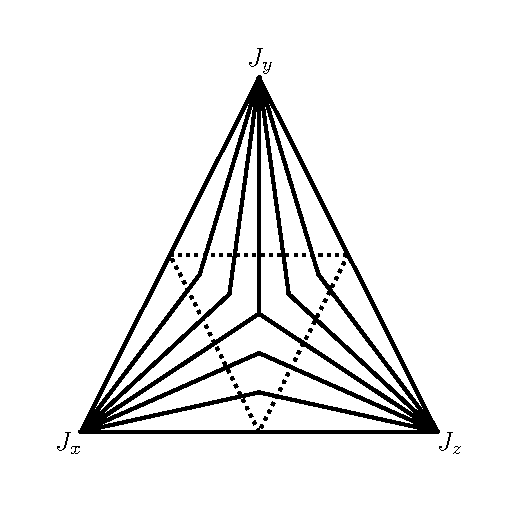
\includegraphics[width=.4\textwidth,height=.4\textheight]{figure_code/logo/logo}
\vspace{-0.4\textheight}
\vspace{10mm}
}
\submitdate{October 2022}

% \normallinespacing

\maketitle

\preface

%The abstract page
\addcontentsline{toc}{chapter}{Abstract}
\begin{abstract}
\input{build/latex/0_Preface/0.1_Abstract.tex}
\end{abstract}

% the page with versions, declaration of originality and copyright
\include{build/latex/0_Preface/0.2_Declarations.tex}

% the Acknodledgemnet page
\cleardoublepage
\addcontentsline{toc}{chapter}{Acknowledgements}
\begin{acknowledgements}
\input{build/latex/0_Preface/0.3_Aknowledgements.tex}
\end{acknowledgements}

% the dedication page
\cleardoublepage
% \begin{dedication}
\vspace*{100mm} % about one third of the vertical of an A4 page
\begin{center}To Kathrin.\end{center}
% \end{dedication}

\body

\hypersetup{
  linkcolor  = urlblue,
  citecolor  = black,
  urlcolor   = urlblue,
  }

\hypertarget{chap:1-introduction}{\chapter{Introduction}}
\begin{refsection}
\hypertarget{interacting-quantum-many-body-systems}{%
\section{Interacting Quantum Many Body Systems}\label{interacting-quantum-many-body-systems}}

When you take many objects and let them interact together, when we describe the behaviours that arise it is often easier to talks in terms of the group rather than the behaviour of the individual objects. A flock of starlings like that of \cref{fig:Studland_Starlings} is a good example. If you were to sit and watch a flock like this, you'd see that it has a distinct outline, that waves of density will sometimes propagate through the closely packed birds and that the flock seems to respond to predators as a distinct object. The natural description of this phenomenon is in terms of the flock, not the individual birds.

A flock is an \emph{emergent phenomenon}. The starlings are only interacting with their immediate six or seven neighbours~\autocite{king2012murmurations,balleriniInteractionRulingAnimal2008}, what a physicist would call a \emph{local interaction}. There is much philosophical debate about how exactly to define emergence~\autocite{andersonMoreDifferent1972,kivelsonDefiningEmergencePhysics2016}. For our purposes, it is enough to say that emergence is the fact that the aggregate behaviour of many interacting objects may necessitate a radically different description from that of the individual objects.

\hypertarget{fig:Studland_Starlings}{%
\begin{figure}
\centering
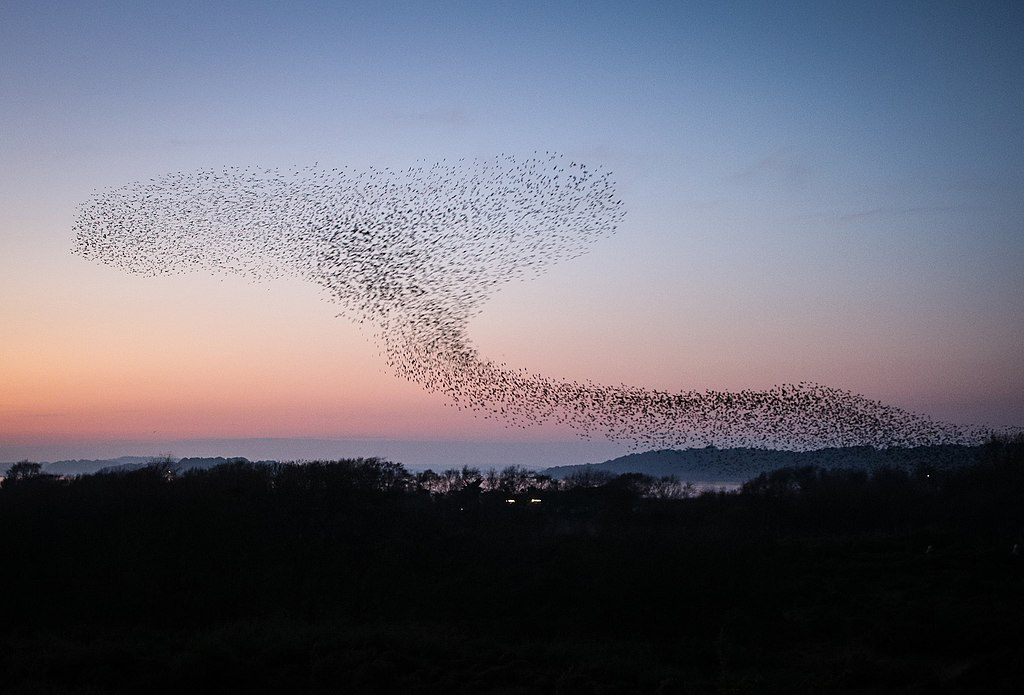
\includegraphics[width=1\textwidth,height=\textheight]{figure_code/intro_chapter/Studland_Starlings.jpeg}
\caption[{A murmuration of Starlings}]{A murmuration of starlings. Dorset, UK. Credit \href{https://twitter.com/arripay}{Tanya Hart}, ``Studland Starlings'', 2017, \href{https://creativecommons.org/licenses/by-sa/3.0/deed.en}{CC BY-SA 3.0}}
\label{fig:Studland_Starlings}
\end{figure}
}

To give an example closer to the topic at hand, our understanding of thermodynamics began with bulk properties like heat, energy, pressure and temperature~\autocite{saslowHistoryThermodynamicsMissing2020}. It was only later that we gained an understanding of how these properties emerge from microscopic interactions between very large numbers of particles~\autocite{flammHistoryOutlookStatistical1998}.

At its heart, condensed matter is the study of the behaviours that can emerge from large numbers of interacting quantum objects at low energy. When these three properties are present together (a large number of objects, those objects being quantum and the presence interactions between the objects), we call it an interacting quantum many body system. From these three ingredients, nature builds all manner of weird and wonderful materials.

Historically, we first made headway by ignoring interactions and quantum properties and looking at purely many-body systems. The ideal gas law and the Drude classical electron gas~\autocite{ashcroftSolidStatePhysics1976} are good examples. Including interactions leads to the Ising model~\autocite{isingBeitragZurTheorie1925}, the Landau theory~\autocite{landau2013fluid} and the classical theory of phase transitions~\autocite{jaegerEhrenfestClassificationPhase1998}. In contrast, condensed matter theory got its start in quantum many-body theory where the only electron-electron interaction considered is the Pauli exclusion principle. Bloch's theorem~\autocite{blochÜberQuantenmechanikElektronen1929}, the core result of band theory, predicted the properties of non-interacting electrons in crystal lattices. It predicted, in particular, that band insulators arise when the electrons bands are filled, leaving the fermi level in a bandgap~\autocite{ashcroftSolidStatePhysics1976}. In the same vein, advances were made in understanding the quantum origins of magnetism, including ferromagnetism and antiferromagnetism~\autocite{MagnetismCondensedMatter}.

The development of Landau-Fermi liquid theory explained why band theory works so well even where an analysis of the relevant energies suggests that it should not~\autocite{wenQuantumFieldTheory2007}. Landau Fermi Liquid theory demonstrates that, in many cases where electron-electron interactions are significant, the system can still be described in terms of generalised non-interacting quasiparticles. This happens when the properties of the quasiparticles in the interacting system can be smoothly connected to the free fermions of the non-interacting system.

However, there are systems where even Landau-Fermi liquid theory fails. An effective theoretical description of these systems must include electron-electron correlations. They are thus called strongly correlated materials~\autocite{morosanStronglyCorrelatedMaterials2012}. The canonical examples are superconductivity~\autocite{MicroscopicTheorySuperconductivity}, the fractional quantum hall effect~\autocite{feldmanFractionalChargeFractional2021} and the Mott insulators~\autocite{mottBasisElectronTheory1949,fisherMottInsulatorsSpin1999}. We'll start by looking at the latter but shall see that there are many links between the three topics.

\hypertarget{mott-insulators}{%
\section{Mott Insulators}\label{mott-insulators}}

Mott Insulators (MIs) are remarkable because their electrical insulator properties come not from having filled bands but from electron-electron interactions other than Pauli exclusion. Electrical conductivity, the bulk movement of electrons, requires both that there are electronic states very close in energy to the ground state and that those states are delocalised so that they can contribute to macroscopic transport. Band insulators are systems whose Fermi level falls within a gap in the density of states and thus fail the first criteria. Band insulators derive their character from the characteristics of the underlying lattice. A third kind of insulator, the Anderson insulators, have only localised electronic states near the fermi level and therefore fail the second criteria. In a later section, I will discuss Anderson insulators and the disorder that drives them.

Both band and Anderson insulators occur without electron-electron interactions. MIs, by contrast, require a many body picture to understand and thus elude band theory and single-particle methods.

\hypertarget{fig:venn_diagram}{%
\begin{figure}
\centering
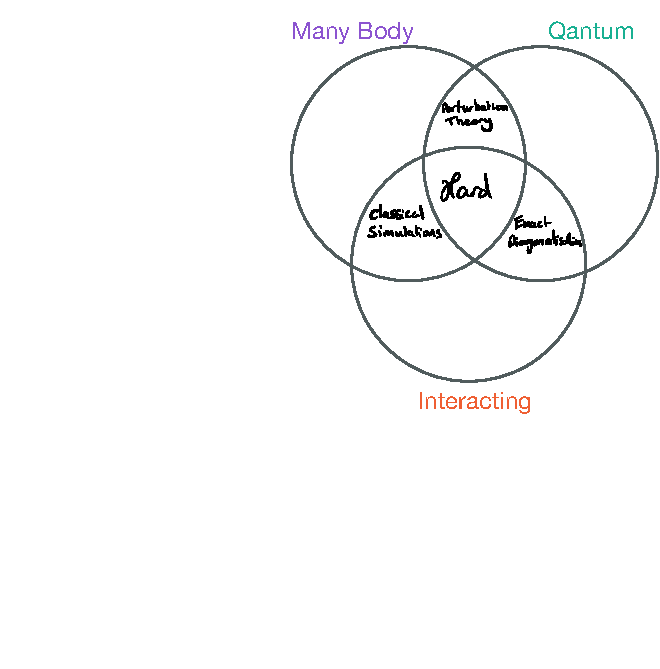
\includegraphics[width=1\textwidth,height=\textheight]{figure_code/intro_chapter/venn_diagram}
\caption[{Interacting Quantum Many Body Systems Venn Diagram}]{Three key adjectives. \emph{Many Body}: systems considered in the limit of large numbers of particles. \emph{Quantum}: objects whose behaviour requires quantum mechanics to describe accurately. \emph{Interacting}: the constituent particles of the system affect one another via forces, either directly or indirectly. When taken together, these three properties can give rise to strongly correlated materials.}
\label{fig:venn_diagram}
\end{figure}
}

The theory of MIs developed out of the observation that band theory erroneously predicts that many transition metal oxides are conductive~\autocite{boerSemiconductorsPartiallyCompletely1937}. It was suggested that electron-electron interactions were the cause of this effect~\autocite{mottDiscussionPaperBoer1937}. Interest grew with the discovery of high temperature superconductivity in the cuprates in 1986~\autocite{bednorzPossibleHighTcSuperconductivity1986} which is believed to arise as the result of a doped MI state~\autocite{leeDopingMottInsulator2006}.

The canonical toy model of the MI is the Hubbard model~\autocite{gutzwillerEffectCorrelationFerromagnetism1963,kanamoriElectronCorrelationFerromagnetism1963,hubbardj.ElectronCorrelationsNarrow1963} of spin-\(1/2\) fermions hopping on the lattice with hopping parameter \(t\) and electron-electron repulsion \(U\)

\[ H_{\mathrm{H}} = -t \sum_{\langle i,j \rangle \alpha} c^\dagger_{i\alpha} c_{j\alpha} + U \sum_i n_{i\uparrow} n_{i\downarrow} - \mu \sum_{i,\alpha} n_{i\alpha},\]

where \(c^\dagger_{i\alpha}\) creates a spin \(\alpha\) electron at site \(i\) and the number operator \(n_{i\alpha}\) measures the number of electrons with spin \(\alpha\) at site \(i\). The sum runs over lattice neighbours \(\langle i,j \rangle\) including both \(\langle i,j \rangle\) and \(\langle j,i \rangle\) so that the model is Hermitian.

In the non-interacting limit \(U << t\), the model reduces to free fermions and the many-body ground state is a separable product of Bloch waves filled up to the Fermi level. On the other hand, the ground state in the interacting limit \(U >> t\) is a direct product of the local Hilbert spaces \(|0\rangle, |\uparrow\rangle, |\downarrow\rangle, |\uparrow\downarrow\rangle\). At half filling, one electron per site, each site becomes a \emph{local moment} in the reduced Hilbert space \(|\uparrow\rangle, |\downarrow\rangle\) and thus acts like a spin-\(1/2\)~\autocite{hubbardElectronCorrelationsNarrow1964}.

The Mott insulating phase occurs at half filling \(\mu = \tfrac{U}{2}\). Here the model can be rewritten in a symmetric form \[ H_{\mathrm{H}} = -t \sum_{\langle i,j \rangle \alpha} c^\dagger_{i\alpha} c_{j\alpha} + U \sum_i (n_{i\uparrow} - \tfrac{1}{2})(n_{i\downarrow} - \tfrac{1}{2}).\]

The basic reason that the half filled state is insulating seems trivial. Any excitation must include states of double occupancy that cost energy \(U\). Hence, the system has a finite bandgap and is an interaction-driven MI. Depending on the lattice, the local moments may then order antiferromagnetically. Originally it was proposed that this Antiferromagnetic (AFM) order was actually the reason for the insulating behaviour. This would make sense since AFM order doubles the unit cell and can turn a system into a band insulator with an even number of electrons per unit cell~\autocite{mottMetalInsulatorTransitions1990}. However, MIs have been found without magnetic order~\autocite{law1TTaS2QuantumSpin2017,ribakGaplessExcitationsGround2017}. Instead, the local moments may form a highly entangled state known as a Quantum Spin Liquid (QSL), which will be discussed shortly.

Various theoretical treatments of the Hubbard model have been made, including those based on Fermi liquid theory, mean field treatments, the local density approximation~\autocite{slaterMagneticEffectsHartreeFock1951}, dynamical mean-field theory~\autocite{greinerQuantumPhaseTransition2002}, density matrix renormalisation group methods~\autocite{hallbergNewTrendsDensity2006,schollwöckDensitymatrixRenormalizationGroup2005,whiteDensityMatrixFormulation1992} and Markov chain Monte Carlo~\autocite{blankenbeclerMonteCarloCalculations1981,hirschDiscreteHubbardStratonovichTransformation1983,whiteNumericalStudyTwodimensional1989}. None of these approaches are perfect. Strong correlations are poorly described by Fermi liquid theory and LDA approaches while mean field approximations do poorly in low dimensional systems. This theoretical difficulty has made the Hubbard model a target for cold atom simulations~\autocite{mazurenkoColdatomFermiHubbard2017}.

From here, the discussion will branch in two directions. First, I will discuss a limit of the Hubbard model called the Falicov-Kimball model. Second, I will look at QSLs and the Kitaev honeycomb model.

\hypertarget{intro-the-fk-model}{%
\subsubsection{The Falicov-Kimball Model}\label{intro-the-fk-model}}

\hypertarget{fig:fk_schematic}{%
\begin{figure}
\centering
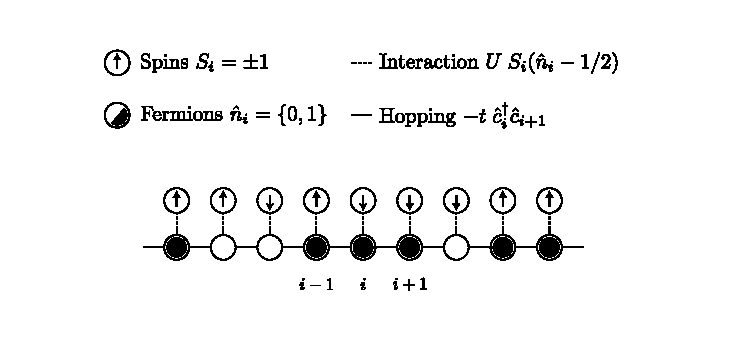
\includegraphics[width=1\textwidth,height=\textheight]{figure_code/intro_chapter/fk_schematic}
\caption[{Falicov-Kimball Model Diagram}]{The Falicov-Kimball model can be viewed as a model of classical spins \(S_i\) coupled to spinless fermions \(\hat{c}_i\) where the fermions are mobile with hopping \(t\) and the fermions are coupled to the spins by an Ising type interaction with strength \(U\).}
\label{fig:fk_schematic}
\end{figure}
}

The Falicov-Kimball (FK) model was originally introduced to describe the metal-insulator transition in f-electron system~\autocite{hubbardj.ElectronCorrelationsNarrow1963,falicovSimpleModelSemiconductorMetal1969}. The FK model is the limit of the Hubbard model as the mass of one of the spins states of the electron is taken to infinity. This gives a model with two fermion species, one itinerant and one entirely immobile. The number operators for the immobile fermions are therefore conserved quantities and can be be treated like classical degrees of freedom. For our purposes, it will be useful to replace the immobile fermions with a classical Ising background field \(S_i = \pm1\).

\[\begin{aligned}
H_{\mathrm{FK}} = & -\;t \sum_{\langle i,j \rangle} c^\dagger_{i}c_{j} + \;U \sum_{i} S_i\;(c^\dagger_{i}c_{i} - \tfrac{1}{2}). \\ 
\end{aligned}\]

The physics of states near the metal-insulator transition is still poorly understood~\autocite{belitzAndersonMottTransition1994,baskoMetalInsulatorTransition2006}. As a result, the FK model provides a rich test bed to explore interaction-driven metal-insulator transition physics. Despite its simplicity, the model has a rich phase diagram in \(D \geq 2\) dimensions. It shows a Mott insulator transition even at high temperature, similar to the corresponding Hubbard model~\autocite{brandtThermodynamicsCorrelationFunctions1989}. In 1D, the ground state phenomenology as a function of filling can be rich~\autocite{gruberGroundStatesSpinless1990}, but the system is disordered for all \(T > 0\)~\autocite{kennedyItinerantElectronModel1986}. The model has also been a test-bed for many-body methods. Interest took off when an exact dynamical mean-field theory solution in the infinite dimensional case was found~\autocite{antipovCriticalExponentsStrongly2014,ribicNonlocalCorrelationsSpectral2016,freericksExactDynamicalMeanfield2003,herrmannNonequilibriumDynamicalCluster2016}.

In~\protect\hyperlink{chap:3-the-long-range-falicov-kimball-model}{chapter 3}, I will introduce a generalised Falicov-Kimball model in 1D I call the Long-Range Falicov-Kimball model. With the addition of long-range interactions in the background field, the model shows a similarly rich phase diagram like its higher dimensional cousins. Our goal is to understand the Mott transition in more detail, the phase transition into a charge density wave state and how the localisation properties of the fermionic sector behave in 1D. We were particularly interested to see if correlations in the disorder potential are enough to bring about localisation effects, such as mobility edges, that are normally only seen in higher dimensions. I use an exact Markov chain Monte Carlo method to map the phase diagram and compute the energy-resolved localisation properties of the fermions. We observe what appears to be a hint of coexisting localised and delocalised states. However, after careful comparison to an Anderson model of uncorrelated binary disorder about a background charge density wave field, we confirm that the fermionic sector does fully localise at larger system sizes as expected for 1D systems.

\hypertarget{quantum-spin-liquids}{%
\section{Quantum Spin Liquids}\label{quantum-spin-liquids}}

Turning to the other key topic of this thesis, we have already discussed the AFM ordering of local moments in the Mott insulating state. Landau-Ginzburg-Wilson theory characterises phases of matter as inextricably linked to the emergence of long-range order via a spontaneously broken symmetry. Within this paradigm, we would not expect any interesting phases of matter not associated with AFM or other long-range order. However, Anderson first proposed in 1973~\autocite{andersonResonatingValenceBonds1973} that, if long-range order is suppressed by some mechanism, it might lead to a liquid-like state even at zero temperature: a QSL.

This QSL state would exist at zero or very low temperatures. Therefore, we would expect quantum effects to be very strong, which will have far reaching consequences. It was the discovery of a different phase, however, that really kickstarted interest in the topic. The fractional quantum Hall state, discovered in the 1980s~\autocite{laughlinAnomalousQuantumHall1983} is an explicit example of an interacting electron system that falls outside of the Landau-Ginzburg-Wilson paradigm\footnote{In fact the FQH state \emph{can} be described within a Ginzburg-Landau like paradigm but it requires a non-local order parameter~\autocite{girvinOffdiagonalLongrangeOrder1987,readOrderParameterGinzburgLandau1989}. Phases like this are said to possess \emph{topological order} defined by the fact that they cannot be smoothly deformed into a product state~\autocite{chenLocalUnitaryTransformation2010,wenQuantumOrdersSymmetric2002}.}. It shares many phenomenological properties with the QSL state. They both exhibit fractionalised excitations, braiding statistics and non-trivial topological properties~\autocite{broholmQuantumSpinLiquids2020}. The many-body ground state of such systems acts as a complex and highly entangled vacuum. This vacuum can support quasiparticle excitations with properties unbound from that of the Dirac fermions of the standard model.

How do we actually make a QSL? Frustration is one mechanism that we can use to suppress magnetic order in spin models~\autocite{TrebstPhysRep2022}. Frustration can be geometric. Triangular lattices, for instance, cannot support AFM order. It can also come about as a result of spin-orbit coupling or other physics. There are also other routes to QSLs besides frustrated spin systems that we will not discuss here~\autocite{balentsNodalLiquidTheory1998,balentsDualOrderParameter1999,linExactSymmetryWeaklyinteracting1998}.

\hypertarget{fig:kitaev-material-phase-diagram}{%
\begin{figure}
\centering
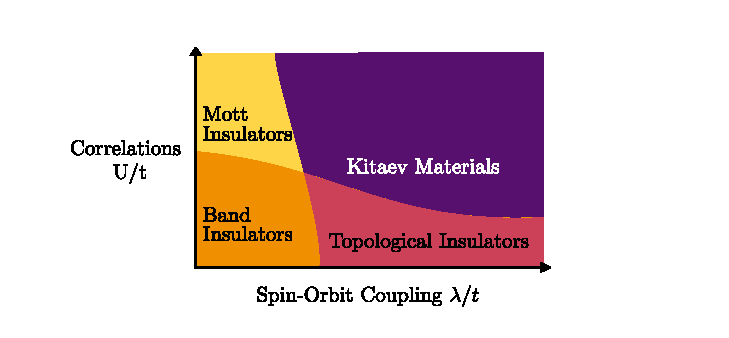
\includegraphics[width=1\textwidth,height=\textheight]{figure_code/intro_chapter/kitaev_material_phase_diagram}
\caption[{Phase Diagram}]{How Kitaev materials fit into the picture of strongly correlated systems. Interactions are required to open a Mott gap and localise the electrons into local moments, while spin-orbit correlations are required to produce the strongly anisotropic spin-spin couplings of the Kitaev model. Reproduced from~\autocite{TrebstPhysRep2022}.}
\label{fig:kitaev-material-phase-diagram}
\end{figure}
}

Spin-orbit coupling is a relativistic effect that, very roughly, corresponds to the fact that in the frame of reference of a moving electron the electric field of nearby nuclei looks like a magnetic field to which the electron spin couples. This couples the spatial and spin parts of the electron wavefunction. The lattice structure can therefore influence the form of the spin-spin interactions, leading to spatial anisotropy in the effective interactions. This spatial anisotropy can frustrate an MI state~\autocite{jackeliMottInsulatorsStrong2009,khaliullinOrbitalOrderFluctuations2005} leading to more exotic ground states than the AFM order we have seen so far. As with the Hubbard model, interaction effects are only strong or weak in comparison to the bandwidth or hopping integral \(t\). Hence, we will see strong frustration in materials with strong spin-orbit coupling \(\lambda\) relative to their bandwidth \(t\).

In certain transition metal based compounds, such as those based on Iridium and Ruthenium, the lattice structure, strong spin-orbit coupling and narrow bandwidths lead to effective spin-\(\tfrac{1}{2}\) Mott insulating states with strongly anisotropic spin-spin couplings. These transition metal compounds, known as Kitaev materials, draw their name from the celebrated Kitaev Honeycomb (KH) model which is expected to model their low temperature behaviour~\autocite{Jackeli2009,HerrmannsAnRev2018,Winter2017,TrebstPhysRep2022,Takagi2019}.

At this point, we can sketch out a phase diagram like that of \cref{fig:kitaev-material-phase-diagram}. When both electron-electron interactions \(U\) and spin-orbit couplings \(\lambda\) are small relative to the bandwidth \(t\), we recover standard band theory of band insulators and metals. In the upper left, we have the simple Mott insulating state as described by the Hubbard model. In the lower right, strong spin-orbit coupling gives rise to topological insulators characterised by symmetry protected edge modes and non-zero Chern number. Kitaev materials occur in the region where strong electron-electron interaction and spin-orbit coupling interact. See~\autocite{witczak-krempaCorrelatedQuantumPhenomena2014} for a more expansive version of this diagram.

The KH model~\autocite{kitaevAnyonsExactlySolved2006} was one of the first exactly solvable spin models with a QSL ground state. It is defined on the 2D honeycomb lattice and provides an exactly solvable model that can be reduced to a free fermion problem via a mapping to Majorana fermions. This yields an extensive number of static \(\mathbb Z_2\) fluxes tied to an emergent gauge field. The model is remarkable not only for its QSL ground state, but also for its fractionalised excitations with non-trivial braiding statistics. It has a rich phase diagram hosting gapless, Abelian and non-Abelian phases~\autocite{knolleDynamicsFractionalizationQuantum2015} and a finite temperature phase transition to a thermal metal state~\autocite{selfThermallyInducedMetallic2019}. It has been proposed that its non-Abelian excitations could be used to support robust topological quantum computing~\autocite{kitaev_fault-tolerant_2003,freedmanTopologicalQuantumComputation2003,nayakNonAbelianAnyonsTopological2008}.

The KH and FK models have quite a bit of conceptual overlap. They can both be seen as models of spinless fermions coupled to a classical Ising background field. This is what makes them exactly solvable. At finite temperatures, fluctuations in their background fields provide an effective disorder potential for the fermionic sector, so both models can be studied at finite temperature with Markov chain Monte Carlo methods~\autocite{antipovInteractionTunedAndersonMott2016,selfThermallyInducedMetallic2019}.

As Kitaev points out in his original paper, the KH model remains solvable on any tri-coordinated \(z=3\) graph which can be 3-edge-coloured. Indeed many generalisations of the model exist~\autocite{Baskaran2007,Baskaran2008,Nussinov2009,OBrienPRB2016,hermanns2015weyl}. Notably, the Yao-Kivelson model~\autocite{yaoExactChiralSpin2007} introduces triangular plaquettes to the honeycomb lattice leading to spontaneous chiral symmetry breaking. These extensions all retain translation symmetry. This is likely because edge-colouring, finding the ground state and understanding the QSL properties are much harder without it~\autocite{eschmann2019thermodynamics,Peri2020}. Undeterred, this gap lead us to wonder what might happen if we remove translation symmetry from the Kitaev model. This would be a model of a tri-coordinated, highly bond anisotropic but otherwise amorphous material.

Amorphous materials do not have long-range lattice regularities but may have short-range regularities in the lattice structure, such as fixed coordination number \(z\) as in some covalent compounds. The best examples are amorphous Silicon and Germanium with \(z=4\) which are used to make thin-film solar cells~\autocite{Weaire1971,betteridge1973possible}. Recently, it has been shown that topological insulating (TI) phases can exist in amorphous systems. Amorphous TIs are characterised by similar protected edge states to their translation invariant cousins and generalised topological bulk invariants~\autocite{mitchellAmorphousTopologicalInsulators2018,agarwala2019topological,marsalTopologicalWeaireThorpeModels2020,costa2019toward,agarwala2020higher,spring2021amorphous,corbae2019evidence}. However, research on amorphous electronic systems has mostly focused on non-interacting systems with a few exceptions, for example, to account for the observation of superconductivity~\autocite{buckel1954einfluss,mcmillan1981electron,meisel1981eliashberg,bergmann1976amorphous,mannaNoncrystallineTopologicalSuperconductors2022} in amorphous materials or very recently to understand the effect of strong electron repulsion in TIs~\autocite{kim2022fractionalization}.

Amorphous \emph{magnetic} systems have been investigated since the 1960s, mostly through the adaptation of theoretical tools developed for disordered systems~\autocite{aharony1975critical,Petrakovski1981,kaneyoshi1992introduction,Kaneyoshi2018} and with numerical methods~\autocite{fahnle1984monte,plascak2000ising}. Research on classical Heisenberg and Ising models accounts for the observed behaviour of ferromagnetism, disordered antiferromagnetism and widely observed spin glass behaviour~\autocite{coey1978amorphous}. However, the role of spin-anisotropic interactions and quantum effects in amorphous magnets has not been addressed.

In~\protect\hyperlink{chap:4-the-amorphous-kitaev-model}{chapter 4}, I will address the question of whether frustrated magnetic interactions on amorphous lattices can give rise to genuine quantum phases, i.e.~to long-range entangled QSL~\autocite{Anderson1973,Knolle2019,Savary2016,Lacroix2011}. We will find that the answer is yes. I will introduce the amorphous Kitaev model, a generalisation of the KH model to random lattices with fixed coordination number three. I will show that this model is a solvable, amorphous, chiral spin liquid. As with the Yao-Kivelson model~\autocite{yaoExactChiralSpin2007}, the amorphous Kitaev model retains its exact solubility but the presence of plaquettes with an odd number of sides leads to a spontaneous breaking of time reversal symmetry. I will confirm prior observations that the form of the ground state is relatively simple~\autocite{OBrienPRB2016,eschmannThermodynamicClassificationThreedimensional2020} and unearth a rich phase diagram displaying Abelian as well as a non-Abelian chiral spin liquid phases. Furthermore, I will show that the system undergoes a finite-temperature phase transition to a thermal metal state and discuss possible experimental realisations.

The next chapter,~\protect\hyperlink{chap:2-background}{Chapter 2}, will introduce some necessary background to the FK model, the KH model, and disorder and localisation.

\printbibliography[heading=subbibintoc]
\end{refsection}

\hypertarget{chap:2-background}{\chapter{Background}}
\begin{refsection}
\begin{Shaded}
\begin{Highlighting}[]
\OperatorTok{\%\%}\NormalTok{html}
\end{Highlighting}
\end{Shaded}

\hypertarget{the-falikov-kimball-model}{%
\section{The Falikov Kimball Model}\label{the-falikov-kimball-model}}

\hypertarget{the-model}{%
\subsection{The Model}\label{the-model}}

discuss CDW phase of 2d model as motivation for studying 1d phase with long range forces

\hypertarget{particle-hole-symmetry}{%
\subsubsection{Particle Hole Symmetry}\label{particle-hole-symmetry}}

\hypertarget{phase-diagram}{%
\subsection{Phase Diagram}\label{phase-diagram}}

\hypertarget{long-range-ising-models}{%
\subsection{Long Range Ising Models}\label{long-range-ising-models}}

\begin{Shaded}
\begin{Highlighting}[]

\end{Highlighting}
\end{Shaded}

\hypertarget{bg-hkm-model}{%
\section{The Kitaev Honeycomb Model}\label{bg-hkm-model}}

\hypertarget{fig:intro_figure_by_hand}{%
\begin{figure}
\centering
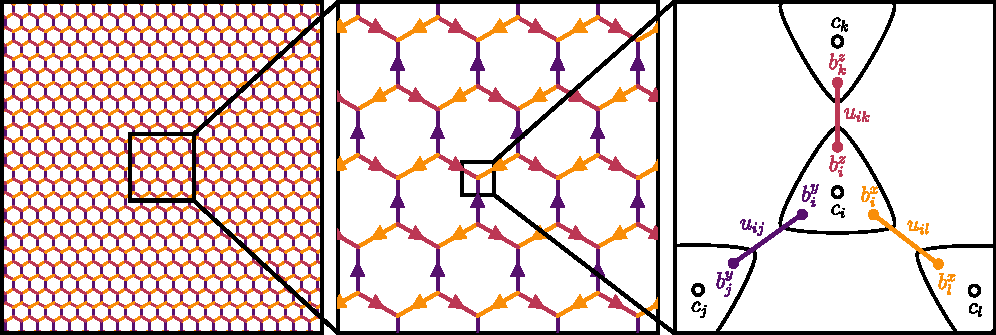
\includegraphics[width=1\textwidth,height=\textheight]{figure_code/amk_chapter/intro/honeycomb_zoom/intro_figure_by_hand}
\caption[{The Kitaev Honeycomb Model}]{\textbf{(a)} The Kitaev honeycomb model is defined on a honeycomb lattice. The special feature of the honeycomb lattice that makes the model solvable is that each vertex is joined by exactly three bonds, i.e.~the lattice is trivalent. One of three labels is assigned to each bond (x,y,z) here represented by colour. \textbf{(b)}. After transforming to the Majorana representation we get an emergent gauge degree of freedom \(u_{jk} = \pm 1\) that lives on each bond, the bond variables. These are antisymmetric, \(u_{jk} = -u_{kj}\), so we represent them graphically with arrows on each bond that point in the direction that \(u_{jk} = +1\) \textbf{(c)}. The Majorana transformation can be visualised as breaking each spin into four Majoranas \(b_i^x,\;b_i^y,\;b_i^z,\;c_i\). The x, y and z Majoranas then pair along the bonds forming conserved \(\mathbb{Z}_2\) bond operators \(u_{jk} = \langle i b_i^\alpha b_j^\alpha \rangle\). The remaining \(c_i\) operators form an effective quadratic Hamiltonian \(H = \frac{i}{4} \sum_{\langle i,j\rangle_\alpha} 2J^{\alpha} u_{ij} \hat{c}_i \hat{c}_j\).}
\label{fig:intro_figure_by_hand}
\end{figure}
}

\hypertarget{the-spin-hamiltonian}{%
\subsection{The Spin Hamiltonian}\label{the-spin-hamiltonian}}

This section introduces the Kitaev honeycomb (KH) model. The KH model is an exactly solvable model of interacting spin\(-1/2\) spins on the vertices of a honeycomb lattice. Each bond in the lattice is assigned a label \(\alpha \in \{ x, y, z\}\) and that bond couple two spins along the \(\alpha\) axis. See \cref{fig:intro_figure_by_hand} for a diagram of the setup.

This gives us the Hamiltonian \begin{equation}\protect\hypertarget{eq:bg-kh-model}{}{ H =  - \sum_{\langle j,k\rangle_\alpha} J^{\alpha}\sigma_j^{\alpha}\sigma_k^{\alpha}, }\label{eq:bg-kh-model}\end{equation} where \(\sigma^\alpha_j\) is the \(\alpha\) component of a Pauli matrix acting on site \(j\) and \(\langle j,k\rangle_\alpha\) is a pair of nearest-neighbour indices connected by an \(\alpha\)-bond with exchange coupling \(J^\alpha\). Kitaev introduced this model in his seminal 2006 paper~\autocite{kitaevAnyonsExactlySolved2006}.

The KH can arise as the result of strong spin-orbit couplings in, for example, the transition metal based compounds~\autocite{Jackeli2009,HerrmannsAnRev2018,Winter2017,TrebstPhysRep2022,Takagi2019}. The model is highly frustrated: each spin would like to align along a different direction with each of its three neighbours. This cannot be achieved even classically~\autocite{chandraClassicalHeisenbergSpins2010,selaOrderbydisorderSpinorbitalLiquids2014}. This frustration leads the the model to have a quantum spin liquid (QSL) ground state, a complex many body state with a high degree of entanglement but no long range magnetic order even at zero temperature. While the possibility of a QSL ground state was suggested much earlier~\autocite{andersonResonatingValenceBonds1973}, the KH model was one of the first concrete models of the QSL state. The KH model has a rich ground state phase diagram with gapless and gapped phases, the latter supporting fractionalised quasiparticles with both Abelian and non-Abelian quasiparticle excitations. Anyons have been the subject of much attention because, among other reasons, they can be braided through spacetime to achieve noise tolerant quantum computations~\autocite{freedmanTopologicalQuantumComputation2003}. At finite temperature the KH model undergoes a phase transition to a thermal metal state~\autocite{selfThermallyInducedMetallic2019}. The KH model can be solved exactly via a mapping to Majorana fermions. This mapping yields an extensive number of static \(\mathbb Z_2\) fluxes tied to an emergent gauge field with the remaining fermions are governed by a free fermion hamiltonian.

This section will go over the standard model in detail, first discussing \protect\hyperlink{the-spin-model}{the spin model}, then detailing the transformation to a \protect\hyperlink{the-majorana-model}{Majorana hamiltonian} that allows a full solution while enlarging the Hamiltonian. We will discuss the properties of the \protect\hyperlink{an-emergent-gauge-field}{emergent gauge fields} and the projector. The \protect\hyperlink{sec:anyons}{next section} will discuss anyons, topology and the Chern number, using the Kitaev model as an explicit example of these topics. Finally will then discuss the ground state found via Lieb's theorem as well as work on generalisations of the ground state to other lattices. Finally we will look at the \protect\hyperlink{ground-state-phases}{phase diagram}.

\hypertarget{the-spin-model}{%
\subsection{The Spin Model}\label{the-spin-model}}

\hypertarget{fig:visual_kitaev_1}{%
\begin{figure}
\centering
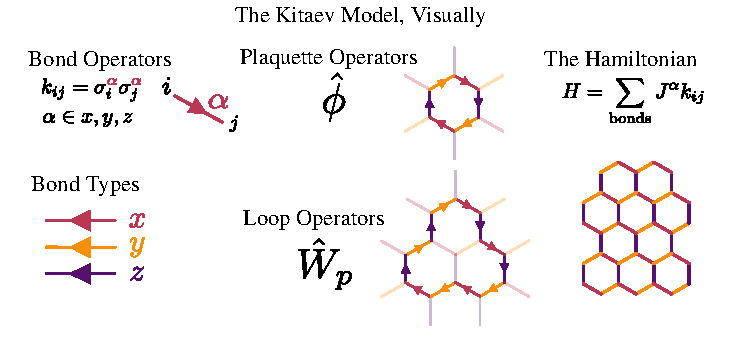
\includegraphics[width=1\textwidth,height=\textheight]{figure_code/amk_chapter/visual_kitaev_1}
\caption[{A Visual Intro to the Kitaev Model}]{A visual introduction to the Kitaev Model.}
\label{fig:visual_kitaev_1}
\end{figure}
}

As discussed in the introduction, spin hamiltonians like that of the Kitaev model arise in electronic systems as the result the balance of multiple effects~\autocite{TrebstPhysRep2022}. For instance, in certain transition metal systems with \(d^5\) valence electrons, crystal field and spin-orbit couplings conspire to shift and split the \(d\) orbitals into moments with spin \(j = 1/2\) and \(j = 3/2\). Of these, the bandwidth \(t\) of the \(j= 1/2\) band is small, meaning that even relatively meagre electron correlations (such those induced by the \(U\) term in the Hubbard model) can lead to the opening of a Mott gap. From there we have a \(j = 1/2\) Mott insulator whose effective spin-spin interactions are again shaped by the lattice geometry and spin-orbit coupling leading some materials to have strong bond-directional Ising-type interactions~\autocite{jackeliMottInsulatorsStrong2009,khaliullinOrbitalOrderFluctuations2005}. In the Kitaev Model the bond directionality refers to the fact that the coupling axis \(\alpha\) in terms like \(\sigma_j^{\alpha}\sigma_k^{\alpha}\) is strongly bond dependent.

In the spin hamiltonian \cref{eq:bg-kh-model} we can already tease out a set of conserved fluxes that will be key to the model's solution. These fluxes are the expectations of Wilson loop operators

\[\hat{W}_p = \prod_{\langle i,j\rangle_\alpha\; \in\; p} \sigma_i^{\alpha}\sigma_j^{\alpha},\]

the products of bonds winding around a closed path \(p\) on the lattice. These operators commute with the Hamiltonian and so have no time dynamics. The winding direction does not matter so long as it is fixed. By convention we will always use clockwise. Each closed path on the lattice is associated with a flux. The number of conserved quantities grows linearly with system size and is thus extensive, this is a common property for exactly solvable systems and can be compared to the heavy electrons present in the Falikov-Kimball model. The square of two loop operators is one so any contractible loop can be expressed as a product of loops around plaquettes of the lattice, as in \cref{fig:stokes_theorem}. For the honeycomb lattice the plaquettes are the hexagons. The expectations of \(\hat{W}_p\) through each plaquette, the fluxes, are therefore enough to describe the whole flux sector. We will focus on these fluxes, denoting them by \(\phi_i\). Once we have made the mapping to the Majorana Hamiltonian I will explain how these fluxes can be connected to an emergent \(B\) field which makes their interpretation as fluxes clear.

\hypertarget{fig:stokes_theorem}{%
\begin{figure}
\centering
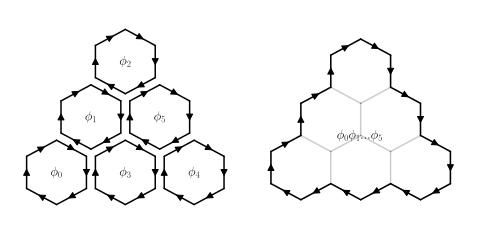
\includegraphics[width=0.71\textwidth,height=\textheight]{figure_code/amk_chapter/stokes_theorem/stokes_theorem}
\caption[{We can construct arbitrary loops from plaquette fluxes.}]{In the Kitaev Honeycomb model, Wilson loop operators \(\hat{W}_p = \prod_{\langle i,j\rangle_\alpha\; \in\; p} \sigma_i^{\alpha}\sigma_j^{\alpha}\) can be composed via multiplication to produce arbitrary contractible loops. As a consequence we need only to keep track of the value of the flux through each plaquette \(\phi_i\). This relationship between the \(u_{ij}\) around a region and fluxes with one is evocative of Stokes' theorem for classical electromagnetism. In fact it turns out to be the exponential of it as we shall make explicit later.}
\label{fig:stokes_theorem}
\end{figure}
}

It is worth noting in passing that the effective Hamiltonian for many Kitaev materials incorporates a contribution from an isotropic Heisenberg term \(\sum_{i,j} \vec{\sigma}_i\cdot\vec{\sigma}_j\), this is referred to as the Heisenberg-Kitaev Model~\autocite{Chaloupka2010}. Materials for which the Kitaev term dominates are generally known as Kitaev Materials. See~\autocite{TrebstPhysRep2022} for a full discussion of Kitaev Materials.

As with the Falikov-Kimball model, the KH model has a extensive number of conserved quantities, the fluxes. As with the FK model it will make sense to work in the simultaneous eigenbasis of the fluxes and the Hamiltonian so that we can treat the fluxes like a classical degree of freedom. This is part of what makes the model tractable. We will find that the ground state of the model corresponds to some particular choice of fluxes. We will refer to local excitations away from the flux ground state as \textbf{vortices}. In order to fully solve the model however, we must first move to a Majorana picture.

\hypertarget{the-majorana-model}{%
\subsection{The Majorana Model}\label{the-majorana-model}}

Majorana fermions are something like `half of a complex fermion' and are their own antiparticle. From a set of \(N\) fermionic creation \(f_i^\dagger\) and anhilation \(f_i\) operators we can construct \(2N\) Majorana operators \(c_m\). We can do this construction in multiple ways subject to only mild constraints required to keep the overall commutations relations correct~\autocite{kitaevAnyonsExactlySolved2006}. Majorana operators square to one but otherwise have standard fermionic commutation relations.

\(N\) spins can be mapped to \(N\) fermions with the well known Jordan-Wigner transformation and indeed this approach can be used to solve the Kitaev model~\autocite{chenExactResultsKitaev2008}. Here I will introduce the method Kitaev used in the original paper as this forms the basis for the results that will be presented in this thesis. Rather than mapping to \(N\) fermions, Kitaev maps to \(4N\) Majoranas, effectively \(2N\) fermions. In contrast to the Jordan-Wigner approach which makes fermions out of strings of spin operators in order to correctly produce fermionic commutation relations, the Kitaev transformation maps each spin locally to four Majoranas. The downside is that this enlarges the Hilbert space from \(2^N\) to \(4^N\). We will have to employ a projector \(\hat{P}\) to come back down to the physical Hilbert space later. As everything is local, I will drop the site indices \(ijk\) in expressions that refer to only a single site.

The mapping is defined in terms of four Majoranas per site \(b_i^x,\;b_i^y,\;b_i^z,\;c_i\) such that

\begin{equation}\protect\hypertarget{eq:bg-kh-mapping}{}{\tilde{\sigma}^x = i b^x c,\; \tilde{\sigma}^y = i b^y c,\; \tilde{\sigma}^z = i b^z c}\label{eq:bg-kh-mapping}\end{equation}

The tildes on the spin operators \(\tilde{\sigma_i^\alpha}\) emphasis that they live in this new extended Hilbert space and are only equivalent to the original spin operators after applying a projector \(\hat{P}\). The form of the projection operator can be understood in a few ways. From a group-theoretic perspective, before projection, the operators \(\{\tilde{\sigma}^x, \tilde{\sigma}^y, \tilde{\sigma}^z\}\) form a representation of the gamma group \(G_{3,0}\). The gamma groups \(G_{p,q}\) have \(p\) generators that square to the identity and \(q\) that square (roughly) to \(-1\). The generators otherwise obey standard anticommutation relations. The well known gamma matrices \(\{\gamma^0, \gamma^1, \gamma^2, \gamma^3\}\) represent \(G_{1,3}\) the quaternions \(G_{0,3}\) and the Pauli matrices \(G_{3,0}\).

The Pauli matrices, however, have the additional property that the \emph{chiral element} \(\sigma^x \sigma^y \sigma^z = i\), this relation is not determined by the group properties of \(G_{3,0}\). Therefore to fully reproduce the algebra of the Pauli matrices we must project into the subspace where \(\tilde{\sigma}^x \tilde{\sigma}^y \tilde{\sigma}^z = i\). The chiral element of the gamma matrices for instance \(\gamma_5 = i\gamma^0 \gamma^1 \gamma^2 \gamma^3\) is of central importance in quantum field theory. See~\autocite{petitjeanChiralityDiracSpinors2020} for more discussion of this group theoretic view.

The projector must project onto the subspace where \(\tilde \sigma^x \tilde \sigma^y \tilde \sigma^z = i\). If we work this through we find that in general \(\tilde \sigma^x \tilde \sigma^y \tilde\sigma^z = iD\) where \(D = b^x b^y b^z c\) must be the identity for every site. In other words, we can only work with \emph{physical states} \(|\phi\rangle\) that satisfy \(D_i|\phi\rangle = |\phi\rangle\) for all sites \(i\). From this we construct an on-site projector \(P_i = \frac{1 + D_i}{2}\) and the overall projector is simply \(P = \prod_i P_i\).

Another way to see what this is doing physically is to explicitly construct the two intermediate fermionic operators \(f\) and \(g\) that give rise to these four Majoranas. Working through the algebra we see that the \(D\) operator corresponds to the fermion parity \(D = -(2n_f - 1)(2n_g - 1)\) where \(n_f,\; n_g\) are the number operators. Expanding the product \(\prod_i P_i\) out, we find that the projector corresponds to a symmetrisation over \(\{u_{ij}\}\) states within a flux sector and and overall fermion parity \(\prod_i D_i\). This tells us that any arbitrary state can be made to have non-zero overlap with the physical subspace via the addition or removal of a single fermion. This implies that in the thermodynamic limit the projection step is not generally necessary to extract physical results, see~\autocite{pedrocchiPhysicalSolutionsKitaev2011} or \protect\hyperlink{app-the-projector}{appendix A.5} for more details.

We can now rewrite the spin hamiltonian in Majorana form with caveat that they are only strictly equivalent after projection. The Ising interactions \(\sigma_j^{\alpha}\sigma_k^{\alpha}\) decouple into the form \(-i (i b^\alpha_i b^\alpha_j) c_i c_j\). We factor out the \emph{bond operators} \(\hat{u}_{ij} = i b^\alpha_i b^\alpha_j\) which are Hermitian and, remarkably, commute with the Hamiltonian and each other.

\[\begin{aligned}
\tilde{H} &=  - \sum_{\langle i,j\rangle_\alpha} J^{\alpha}\tilde{\sigma}_i^{\alpha}\tilde{\sigma}_j^{\alpha}\\
          &=  i \sum_{\langle i,j\rangle_\alpha} J^{\alpha} \hat{u}_{ij} \hat{c}_i \hat{c}_j
\end{aligned}\]

The bond operators \(\hat{u}_{ij}\) square to one so have eigenvalues \(\pm1\). As they're conserved we will work in their eigenbasis and take off the hats in the Hamiltonian.

\begin{equation}\protect\hypertarget{eq:bg-kh-maj-model}{}{\begin{aligned}
H &=  i \sum_{\langle i,j\rangle_\alpha} J^{\alpha} u_{ij} \hat{c}_i \hat{c}_j
\end{aligned}}\label{eq:bg-kh-maj-model}\end{equation}

\hypertarget{the-fermion-problem}{%
\subsection{The Fermion Problem}\label{the-fermion-problem}}

We now have a quadratic Hamiltonian, \cref{eq:bg-kh-maj-model}, coupled to a classical field \(u_{ij}\). What follows is relatively standard theory for quadratic Hamiltonians~\autocite{BlaizotRipka1986}.

Because of the antisymmetry \(J^{\alpha} u_{ij}\), the eigenvalues of \cref{eq:bg-kh-maj-model} come in pairs \(\pm \epsilon_m\). We organise the eigenmodes of \(H\) into pairs, such that \(b_m\) and \(b_m'\) have energies \(\epsilon_m\) and \(-\epsilon_m\). The transformation \(Q\) \[(c_1, c_2... c_{2N}) Q = (b_1, b_1', b_2, b_2' ... b_{N}, b_{N}')\] puts the Hamiltonian into normal mode form \[\tilde{H}_u = \frac{i}{2} \sum_m \epsilon_m b_m b_m'.\]

The determinant of \(Q\) appears when evaluating the projector explicitly, otherwise, the \(b_m\) are merely an intermediate step. From them, we form fermionic operators \[ f_i = \tfrac{1}{2} (b_m + ib_m')\] with their associated number operators \(n_i = f^\dagger_i f_i\). These let us write the Hamiltonian neatly as

\[ \tilde{H}_u = \sum_m \epsilon_m (n_m - \tfrac{1}{2}).\]

The ground state \(|n_m = 0\rangle\) of the many body system at fixed \(\{u_{ij}\}\) is

\[E_{u,0} = -\frac{1}{2}\sum_m \epsilon_m \]

and we can construct any state from a particular choice of \(n_m = 0,1\).

\hypertarget{an-emergent-gauge-field}{%
\subsection{An Emergent Gauge Field}\label{an-emergent-gauge-field}}

We have transformed the spin Hamiltonian into a Majorana hamiltonian \(H = i \sum_{\langle i,j\rangle_\alpha} J^{\alpha} u_{ij} \hat{c}_i \hat{c}_j\) describing the dynamics of a classical field \(u_{ij}\) and Majoranas \(c_i\). It is natural to ask how the classical field \(u_{ij}\) relates to the fluxes of the original spin model. We can evaluate the fluxes \(\phi_i\) in terms of the bond operators

\begin{equation}\protect\hypertarget{eq:flux-majorana}{}{\phi_i = \prod_{\langle j,k\rangle \in \mathcal{P}_i} i u_{jk}.}\label{eq:flux-majorana}\end{equation}

\hypertarget{fig:gauge_symmetries}{%
\begin{figure}
\centering
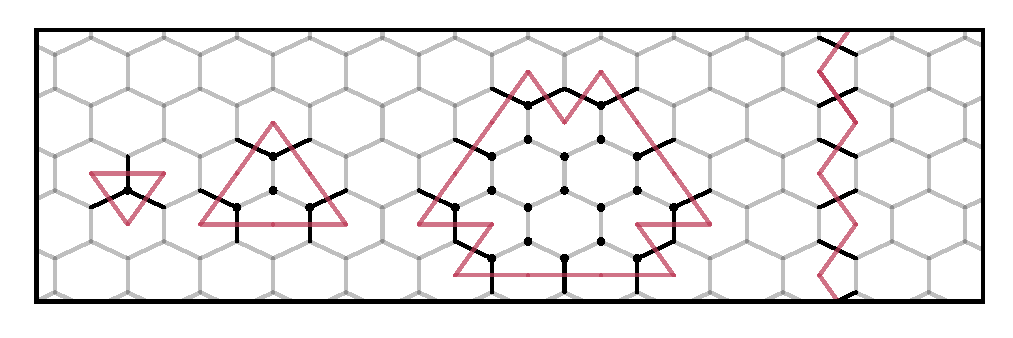
\includegraphics[width=1\textwidth,height=\textheight]{figure_code/amk_chapter/intro/gauge_symmetries/gauge_symmetries}
\caption[{Gauge Symmetries}]{A honeycomb lattice with edges in light grey, along with its dual, the triangle lattice in light blue. The vertices of the dual lattice are the faces of the original lattice and, hence, are the locations of the vortices. (Left) The action of the gauge operator \(D_j\) at a vertex is to flip the value of the three \(u_{jk}\) variables (black lines) surrounding site \(j\). The corresponding edges of the dual lattice (red lines) form a closed triangle. (Middle) Composing multiple adjacent \(D_j\) operators produces a large closed dual loop or multiple disconnected dual loops. Dual loops are not directed like Wilson loops. (Right) A non-contractable loop which cannot be produced by composing \(D_j\) operators. All three operators can be thought of as the action of a vortex-vortex pair that is created, one of them is transported around the loop, and then the two annihilate again. Note that every plaquette has an even number of \(u_{ij}\)s flipped on its edge. Therefore, all retain the same flux \(\phi_i\).}
\label{fig:gauge_symmetries}
\end{figure}
}

In addition, the bond operators form a highly degenerate description of the system. The operators \(D_i = b^x_i b^y_i b^z_i c_i\) commute with \(H\) so form a set of local symmetries. The action of \(D_i\) on a state is to flip the values of the three \(u_{ij}\) bonds that connect to site \(i\). This changes the bond configuration \(\{u_{ij}\}\) but leaves the flux configuration \(\{\phi_i\}\) unchanged. Physically, we interpret \(u_{ij}\) as a gauge field with a high degree of degeneracy and \(\{D_i\}\) as the set of gauge symmetries. The Majorana bond operators \(u_{ij}\) are an emergent, classical, \(\mathbb{Z_2}\) gauge field! The flux configuration \(\{\phi_i\}\) is what encodes physical information about the system.

The ground state of the Kitaev Honeycomb model has flux configuration \(\{\phi_i = +1\}\). This can be proven via Lieb's theorem~\autocite{lieb_flux_1994} which gives the gives the lowest energy magnetic flux configuration for a system of electrons hopping in a magnetic field. Kitaev remarks in his original paper that he was not initially aware of the relevance of Lieb's 1994 result. This is not surprising because at first glance the two models seem quite different but the connection is quite instructive to understanding the Kitaev Model and its generalisations.

Lieb discusses a model of mobile electrons

\[H = \sum_{ij} t_{ij} c^\dagger_i c_j\]

where the hopping term \(t_{ij} = |t_{ij}|\exp(i\theta_{ij})\) incorporate Aharanhov-Bohm~\autocite{aharonovSignificanceElectromagneticPotentials1959} (AB) phases \(\theta_{ij}\). The AB phases model the effect of a slowly varying magnetic field on the electrons through the integral of the magnetic vector potential \(\theta_{ij} = \int_i^j \vec{A} \cdot d\vec{l}\), a Peierls substitution~\autocite{peierlsZurTheorieDiamagnetismus1933}. If we map the Majorana form of the Kitaev model to Lieb's model we see that the \(u_{ij} = \pm 1\) correspond to AB phases \(\theta_{ij} = 0,\pi\) along each bond. Stokes' theorem tells us that the magnetic flux \(\tilde{\phi}_m\) through a surface \(S\) is related to the line integral of \(\vec{A}\) along the boundary of the surface \(\partial S\) which in the discrete case reduces to the sum of the AB phases along the path. We can thus rewrite \cref{eq:flux-majorana} as

\begin{equation}\protect\hypertarget{eq:flux-magnetic}{}{\begin{aligned}
\phi_i &= i^n \prod_{\mathcal{P}_i} \exp{(i\theta_{jk}})\\
       &= i^n \exp \left( i \sum_{\mathcal{P}_i} \theta_{jk} \right)\\
       &= i^n \exp \left( i \oint_{\mathcal{P}_i} \vec{A} \cdot d\vec{l} \right)
\end{aligned}}\label{eq:flux-magnetic}\end{equation}

Thus we can interpret the fluxes \(\phi_i\) as the exponential of magnetic fluxes of some fictitious gauge field \(\vec{A}\) and the bond operators as \(u_{ij} = \exp i \int_i^j \vec{A} \cdot d\vec{l}\). In this analogy to classical electromagnetism, the sets \(\{u_ij\}\) that correspond to the same \(\{\phi_i\}\) are all gauge equivalent. The fact that fluxes can be written as products of bond operators and composed is a consequence of (the exponential of) Stokes' theorem. The additional phase factors of \(i^n\) can be incorporated as additional \(\tfrac{\pi}{2}\) phases but then make little difference when all the plaquettes are hexagons or have an even number of sides. However if the lattice contains odd plaquettes, as in the Yao-Kivelson model~\autocite{yaoExactChiralSpin2007}, the complex fluxes that appear are a sign that chiral symmetry has been broken.

Understanding \(u_{ij}\) as a gauge field provides another way to understand the action of the projector. The local projector \(P_i = \frac{1 + D_i}{2}\) applied to a state constructs a superposition of the original state and the gauge equivalent state linked to it by flipping the three \(u_{ij}\) around site \(i\). The overall projector \(P = \prod_i P_i\) can thus be understood as a symmetrisation over all gauge equivalent states, removing the gauge degeneracy introduced by the mapping from spins to Majoranas.

\hypertarget{fig:topological_fluxes}{%
\begin{figure}
\centering
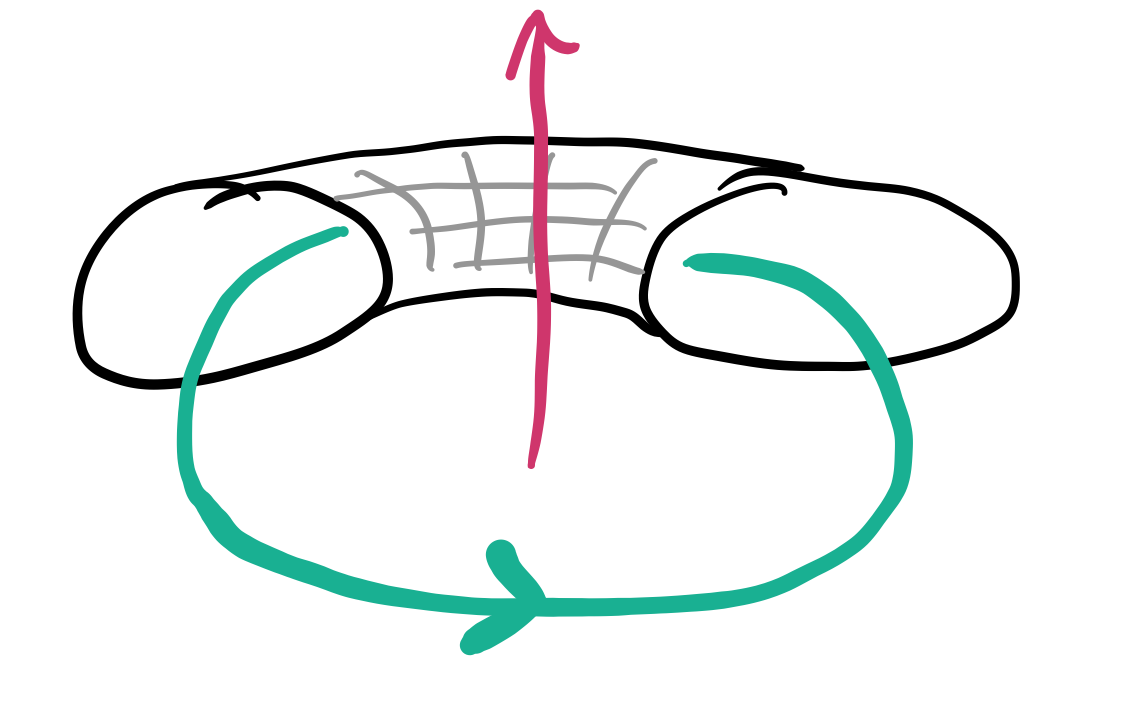
\includegraphics[width=0.57\textwidth,height=\textheight]{figure_code/amk_chapter/topological_fluxes.png}
\caption[{Topological Fluxes}]{Wilson loops that wind the major or minor diameters of the torus measure flux winding through the hole of the doughnut/torus or through the filling. If they made doughnuts with both had a jam filling and a hole, this analogy would be a lot easier to make~\autocite{parkerWhyDoesThis}.}
\label{fig:topological_fluxes}
\end{figure}
}

A final but important point to mention is that is that the local fluxes \(\phi_i\) are not quite all there is. We've seen that products of \(\phi_i\) can be used to construct the flux associated with arbitrary contractible loops. On the plane contractible loops are all there are. However, on the torus we can construct two global fluxes \(\Phi_x\) and \(\Phi_y\) which correspond to paths tracing the major and minor axes. The four sectors spanned by the \(\pm1\) values of these fluxes are gapped away from one another but only by virtual tunnelling processes so the gap decays exponentially with system size~\autocite{kitaevAnyonsExactlySolved2006}. Physically \(\Phi_x\) and \(\Phi_y\) could be thought of as measuring the flux that threads through the hole of the doughnut. In general, surfaces with genus \(g\) have \(g\) `handles' and \(2g\) of these global fluxes. At first glance it may seem this would not have much relevance to physical realisations of the Kitaev model that will likely have a planar geometry with open boundary conditions. However these fluxes are closely linked to topology and the existence of anyonic quasiparticle excitations in the model, which we will discuss next.

\hypertarget{sec:anyons}{%
\subsection{Anyons, Topology and the Chern number}\label{sec:anyons}}

\hypertarget{fig:braiding}{%
\begin{figure}
\centering
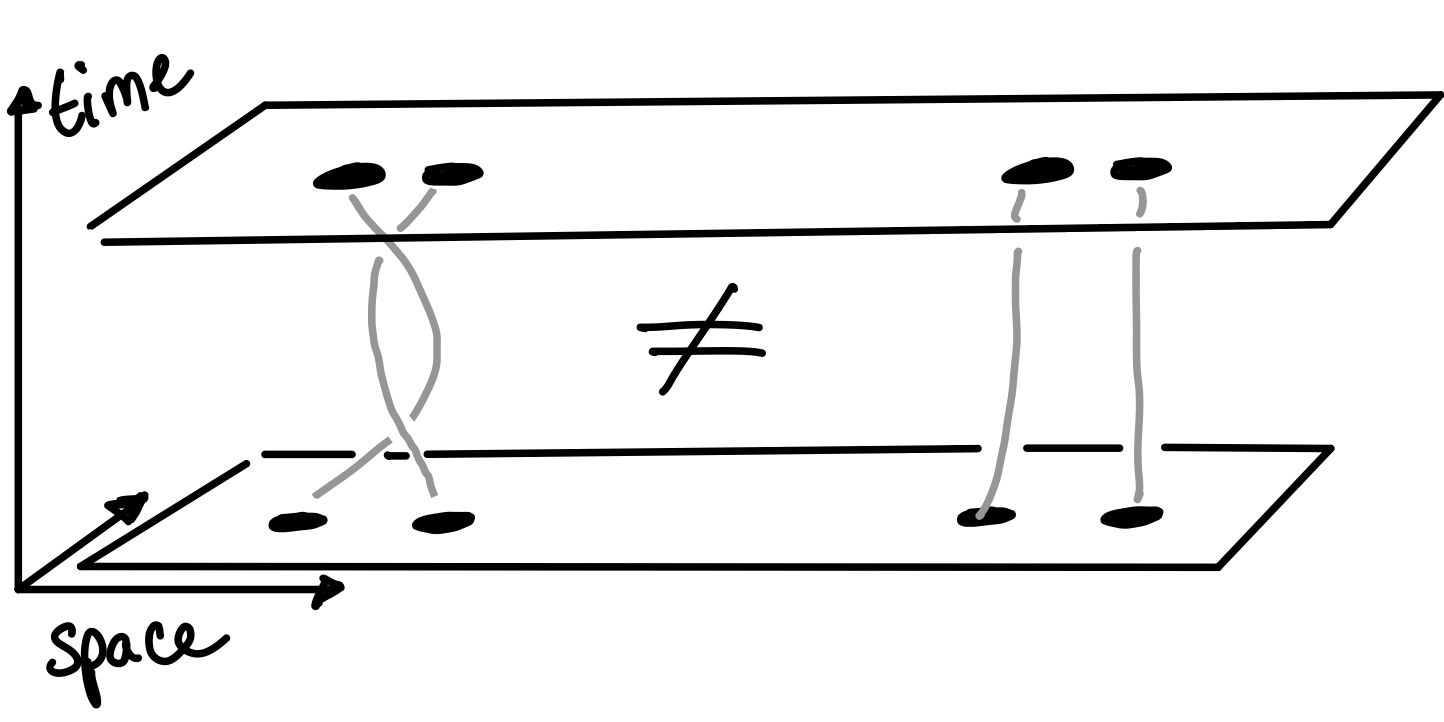
\includegraphics[width=0.71\textwidth,height=\textheight]{figure_code/amk_chapter/braiding.png}
\caption[{Braiding in Two Dimensions}]{Worldlines of particles in two dimensions can become tangled or \emph{braided} with one another.}
\label{fig:braiding}
\end{figure}
}

To discuss different ground state phases of the KH model we must first review the topic of anyons and topology. The standard argument for the existence of Fermions and Bosons goes like this: the quantum state of a system must pick up a factor of \(\pm1\) if two identical particles are swapped. Only \(\pm1\) are allowed since swapping twice must correspond to the identity. This argument works in three dimensions for states without topological degeneracy, which seems to be true of the real world, but condensed matter systems are subject to no such constraints.

In gapped condensed matter systems, all equal time correlators decay exponentially with distance~\autocite{hastingsLiebSchultzMattisHigherDimensions2004}. Put another way, gapped systems support quasiparticles with a definite location in space and finite extent. As such it is meaningful to consider what would happen to the overall quantum state if we were to adiabatically carry out a series of swaps as described above. This is known as braiding.

First we realise that in two dimensions, swapping identical particles twice is not topologically equivalent to the identity, see \cref{fig:braiding}. Instead it corresponds to encircling one particle around the other. This means we can in general pick up any complex phase \(e^{i\theta}\), hence the name \textbf{any}-ons upon exchange. These are known as Abelian anyons because complex multiplication commutes and hence the group of braiding operations forms and Abelian group.

The KH model has a topologically degenerate ground state with sectors labelled by the values of the topological fluxes \((\Phi_x\), \(\Phi_y)\). Consider the operation in which a quasiparticle pair is created from the ground state, transported around one of the non-contractible loops and then annihilated together, call them \(\mathcal{T}_{x}\) and \(\mathcal{T}_{y}\). These operations move us around within the ground state manifold and they need not commute. This leads to non-Abelian anyons. As Kitaev points out, these operations are not specific to the torus: the operation \(\mathcal{T}_{x}\mathcal{T}_{y}\mathcal{T}_{x}^{-1}\mathcal{T}_{y}^{-1}\) corresponds to an operation in which none of the particles crosses the torus, rather one simply winds around the other, hence these effects of relevant even for the planar case.

In condensed matter systems, the existence of anyonic excitations automatically implies the system has topological ground state degeneracy on the torus~\autocite{einarssonFractionalStatisticsTorus1990} and indeed anyons and topology are intimately linked~\autocite{oshikawaTopologicalDegeneracyNonAbelian2007,Chung_Topological_quantum2010,yaoAlgebraicSpinLiquid2009}. Originally a concept used to describe complex vector bundles in algebraic topology~\autocite{chernCharacteristicClassesHermitian1946}, the Chern number has found use in physics as a powerful tool diagnostic tool for topological systems. Kitaev showed that vortices in the KH model are Abelian when the Chern number is even and non-Abelian when the Chern number is odd. In the odd case the non-Abelian statistics of the vortices arise due to unpaired Majorana modes that are bound to them.

Recently, topological systems have gained interest because of proposals to use their ground state degeneracy to implement both passively fault tolerant and actively stabilised quantum computations~\autocite{kitaev_fault-tolerant_2003,poulinStabilizerFormalismOperator2005,hastingsDynamicallyGeneratedLogical2021}.

\hypertarget{ground-state-phases}{%
\subsection{Ground State Phases}\label{ground-state-phases}}

\hypertarget{fig:KH_phase_diagram}{%
\begin{figure}
\centering
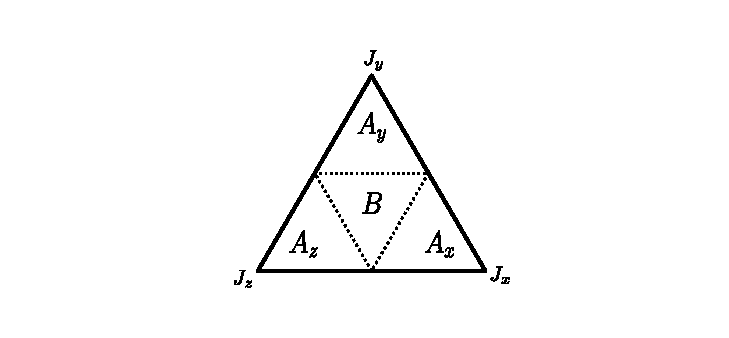
\includegraphics[width=1\textwidth,height=\textheight]{figure_code/background_chapter/KH_phase_diagram}
\caption[{Kitaev Honeycomb Model Phase Diagram}]{Setting the energy scale of the Kitaev Model with the constraint that \(J_x + J_y + J_z = 1\) yields a triangular phase diagram where each of the corners represents \(J_\alpha = 1\). For each corner \(\alpha\) the region \(|J_\alpha > |J_\beta| + |J_\gamma|\) supports a gapped non-Abelian phase equivalent to that of the Toric code~\autocite{kitaev1997quantum,kitaev_fault-tolerant_2003}. The point around equal coupling \(J_x = J_y = J_z\), the B phase, is gapless. The B phase is known a Majorana metal and on the honeycomb lattice it has a Dirac cone dispersion similar to that of graphene.}
\label{fig:KH_phase_diagram}
\end{figure}
}

Setting the overall energy scale with the constraint \(J_x + J_y + J_z = 1\) yields a triangular phase diagram. In each of the corners one of the spin-coupling directions dominates, \(|J_\alpha > |J_\beta| + |J_\gamma|\), yielding three equivalent \(A_\alpha\) phases while the central triangle around \(J_x = J_y = J_z\) is called the B phase. Both phases support two kinds of quasiparticles, fermions and \(\mathbb{Z}_2\)-vortices. In the A phases, the vortices have bosonic statistics with respect to themselves but act like fermions with respect to the fermions, hence they are Abelian anyons, This phase has the same anyonic structure as the Toric code~\autocite{kitaev_fault-tolerant_2003}. Since the B phase is gapless, the quasiparticles aren't localised and so don't have braiding statistics.

An external magnetic can be used to break chiral symmetry. The lowest order term that breaks chiral symmetry but retains the solvability of the model is the three spin term \[
\sum_{(i,j,k)} \sigma_i^{\alpha} \sigma_j^{\beta} \sigma_k^{\gamma}
\] where the sum \((i,j,k)\) runs over consecutive indices around plaquettes. The addition of this to the spin model leads to two bond terms in the corresponding Majorana model. The effect of breaking chiral symmetry is to open a gap in the B phase. The vortices of the gapped B phase are non-Abelian anyons.

At finite temperatures, recent work has shown that the KH model undergoes a transition to a thermal metal phase.

To surmise, the Kitaev Honeycomb model is remarkable because it combines three key properties. First, the form of the Hamiltonian plausibly be realised by a real material. Candidate materials, such as \(\alpha\mathrm{-RuCl}_3\), are known to have sufficiently strong spin-orbit coupling and the correct lattice structure to behave according to the Kitaev Honeycomb model with small corrections~\autocite{banerjeeProximateKitaevQuantum2016,TrebstPhysRep2022}. Second, its ground state is the canonical example of the long sought after quantum spin liquid state, its dynamical spin-spin correlation functions are zero beyond nearest neighbour separation~\autocite{baskaranExactResultsSpin2007}. Its excitations are anyons, particles that can only exist in two dimensions that break the normal fermion/boson dichotomy.

Third, and perhaps most importantly, this model is a rare many body interacting quantum system that can be treated analytically. It is exactly solvable. We can explicitly write down its many body ground states in terms of single particle states~\autocite{kitaevAnyonsExactlySolved2006}. The solubility of the Kitaev Honeycomb Model, like the Falikov-Kimball model of chapter 1, comes about because the model has extensively many conserved degrees of freedom. These conserved quantities can be factored out as classical degrees of freedom, leaving behind a non-interacting quantum model that is easy to solve.

\begin{Shaded}
\begin{Highlighting}[]

\end{Highlighting}
\end{Shaded}

\hypertarget{bg-disorder-and-localisation}{%
\section{Disorder and Localisation}\label{bg-disorder-and-localisation}}

\hypertarget{localisation-anderson-many-body-and-disorder-free}{%
\subsection{Localisation: Anderson, Many Body and Disorder-Free}\label{localisation-anderson-many-body-and-disorder-free}}

\hypertarget{disorder-and-spin-liquids}{%
\subsection{Disorder and Spin liquids}\label{disorder-and-spin-liquids}}

\hypertarget{amorphous-magnetism}{%
\subsection{Amorphous Magnetism}\label{amorphous-magnetism}}

\begin{Shaded}
\begin{Highlighting}[]

\end{Highlighting}
\end{Shaded}

\hypertarget{localisation}{%
\subsection{Localisation}\label{localisation}}

The discovery of localisation in quantum systems surprising at the time given the seeming ubiquity of extended Bloch states. Later, when thermalisation in quantum systems gained interest, localisation phenomena again stood out as counterexamples to the eigenstate thermalisation hypothesis~\autocite{abaninRecentProgressManybody2017,srednickiChaosQuantumThermalization1994}, allowing quantum systems to avoid to retain memory of their initial conditions in the face of thermal noise.

The simplest and first discovered kind is Anderson localisation, first studied in 1958~\autocite{andersonAbsenceDiffusionCertain1958} in the context of non-interacting fermions subject to a static or quenched disorder potential \(V_j\) drawn uniformly from the interval \([-W,W]\)

\[
H = -t\sum_{\langle jk \rangle} c^\dagger_j c_k + \sum_j V_j c_j^\dagger c_j
\]

this model exhibits exponentially localised eigenfunctions \(\psi(x) = f(x) e^{-x/\lambda}\) which cannot contribute to transport processes. Initially it was thought that in one dimensional disordered models, all states would be localised, however it was later shown that in the presence of correlated disorder, bands of extended states can exist~\autocite{izrailevLocalizationMobilityEdge1999,croyAndersonLocalization1D2011,izrailevAnomalousLocalizationLowDimensional2012}.

Later localisation was found in interacting many-body systems with quenched disorder:

\[
H = -t\sum_{\langle jk \rangle} c^\dagger_j c_k + \sum_j V_j c_j^\dagger c_j + U\sum_{jk} n_j n_k
\]

where the number operators \(n_j = c^\dagger_j c_j\). Here, in contrast to the Anderson model, localisation phenomena can be proven robust to weak perturbations of the Hamiltonian. This is called many-body localisation (MBL)~\autocite{imbrieManyBodyLocalizationQuantum2016}.

Both MBL and Anderson localisation depend crucially on the presence of quenched disorder. This has led to ongoing interest in the possibility of disorder-free localisation, in which the disorder necessary to generate localisation is generated entirely from the dynamics of the model. This contracts with typical models of disordered systems in which disorder is explicitly introduced into the Hamilton or the initial state.

The concept of disorder-free localisation was first proposed in the context of Helium mixtures~\autocite{kagan1984localization} and then extended to heavy-light mixtures in which multiple species with large mass ratios interact. The idea is that the heavier particles act as an effective disorder potential for the lighter ones, inducing localisation. Two such models~\autocite{yaoQuasiManyBodyLocalizationTranslationInvariant2016,schiulazDynamicsManybodyLocalized2015} instead find that the models thermalise exponentially slowly in system size, which Ref.~\autocite{yaoQuasiManyBodyLocalizationTranslationInvariant2016} dubs Quasi-MBL.

True disorder-free localisation does occur in exactly solvable models with extensively many conserved quantities~\autocite{smithDisorderFreeLocalization2017}. As conserved quantities have no time dynamics this can be thought of as taking the separation of timescales to the infinite limit.

-link to the FK model

-link to the Kitaev Model

-link to the physics of amorphous systems

\printbibliography[heading=subbibintoc]
\end{refsection}

\hypertarget{chap:3-the-long-range-falicov-kimball-model}{\chapter{The Long-Range Falicov-Kimball Model}}
\backgroundsetup{scale = 1, angle = 0, opacity = 1,
  contents = {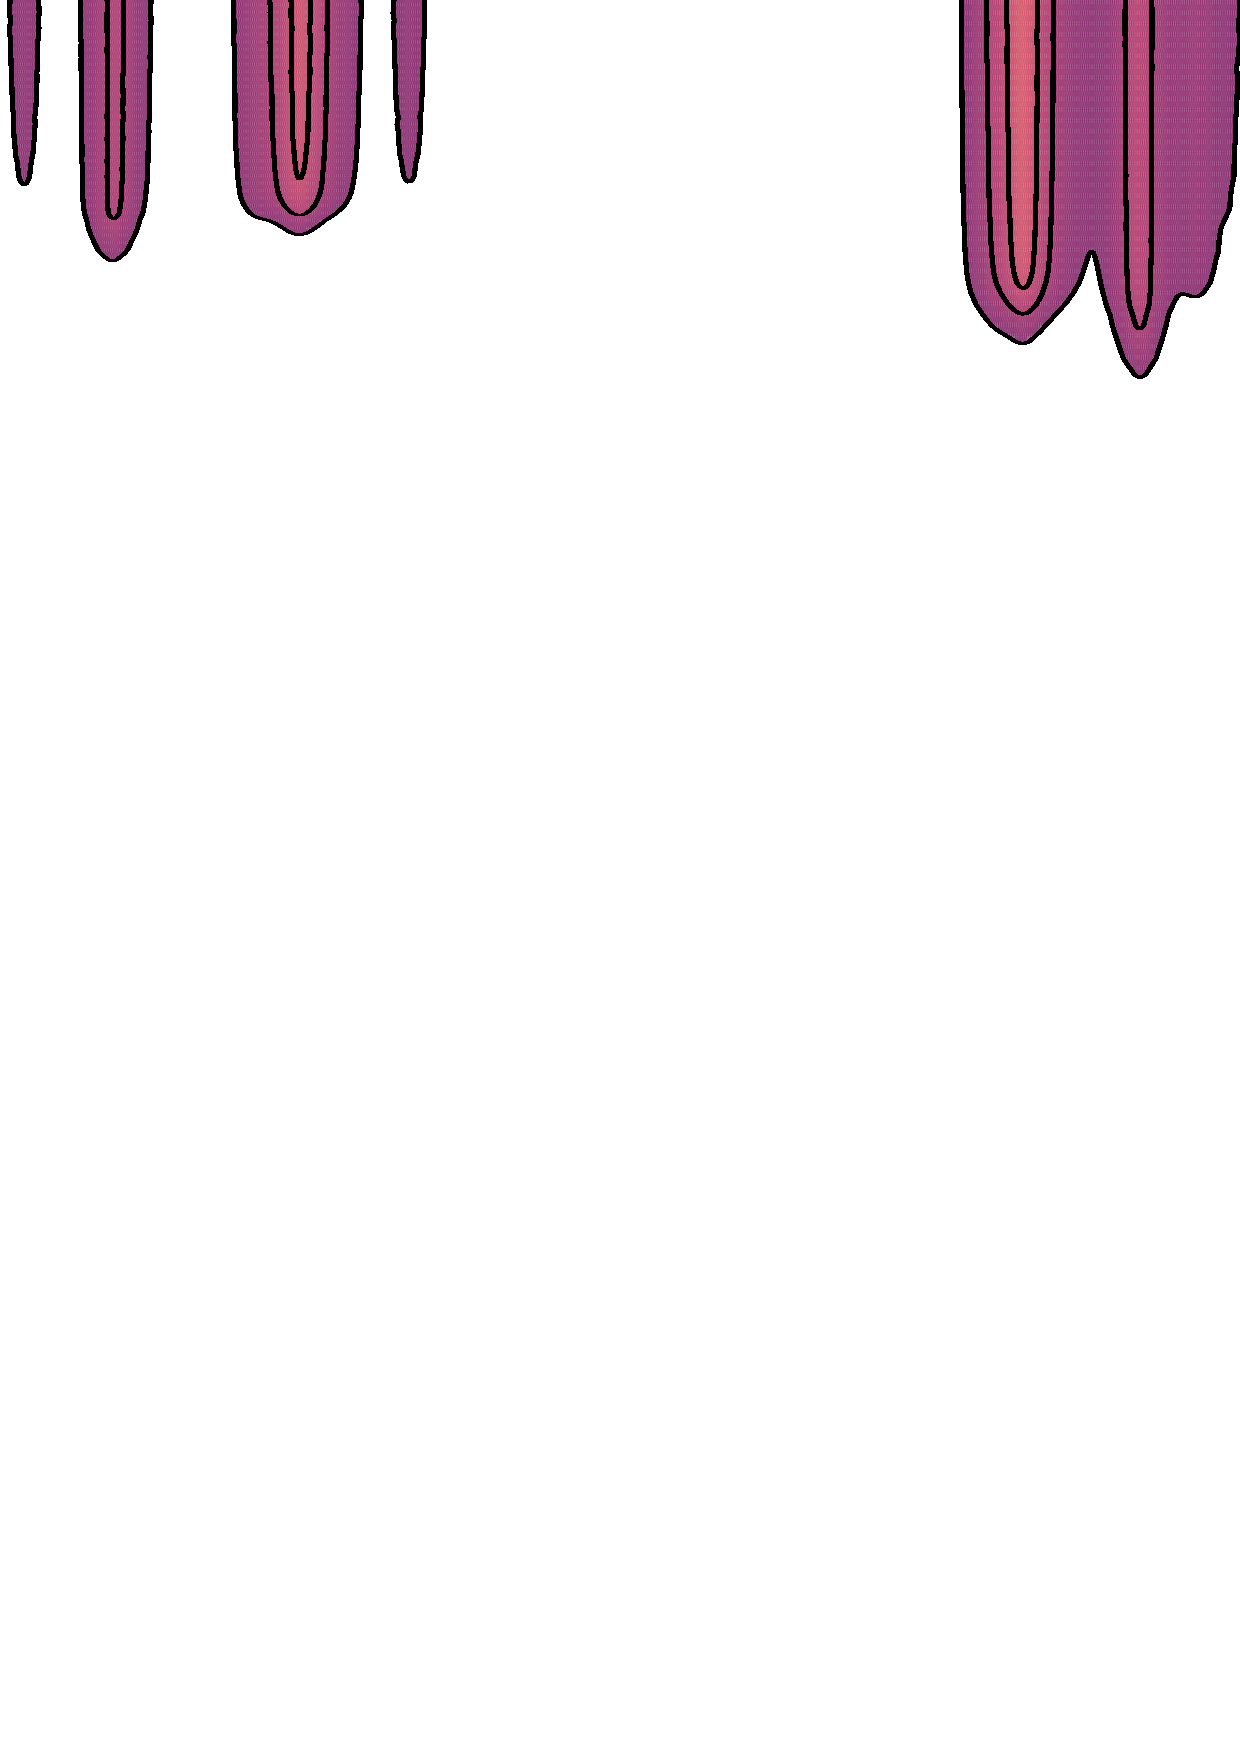
\includegraphics[width=297mm, height=297mm]{figure_code/fk_chapter_background_3.pdf}}}
\BgThispage
\begin{refsection}
\textbf{Contributions}

This chapter expands on work presented in

~\autocite{hodsonOnedimensionalLongrangeFalikovKimball2021} \href{https://link.aps.org/doi/10.1103/PhysRevB.104.045116}{One-dimensional long-range Falikov-Kimball model: Thermal phase transition and disorder-free localization}, Hodson, T. and Willsher, J. and Knolle, J., Phys. Rev.~B, \textbf{104}, 4, 2021,

The code is available online~\autocite{hodsonMCMCFKModel2021}.

Johannes had the initial idea to use a long range Ising term to stabilise order in a one dimension Falikov-Kimball model. Josef developed a proof of concept during a summer project at Imperial along with Alexander Belcik. I wrote the simulation code and performed all the analysis presented here.

\textbf{Chapter Summary}

The paper is organised as follows. First, I will introduce the long range Falicov-Kimball (LRFK) model and motivate its definition. Second, I will present the~\protect\hyperlink{sec:lrfk-methods}{methods} used to solve it numerically, including Markov chain Monte Carlo and finite size scaling. I will then present and interpret the~\protect\hyperlink{sec:lrfk-results}{results} obtained.

\hypertarget{sec:lrfk-model}{%
\section{The Model}\label{sec:lrfk-model}}

\hypertarget{fig:lrfk_schematic}{%
\begin{figure}
\centering
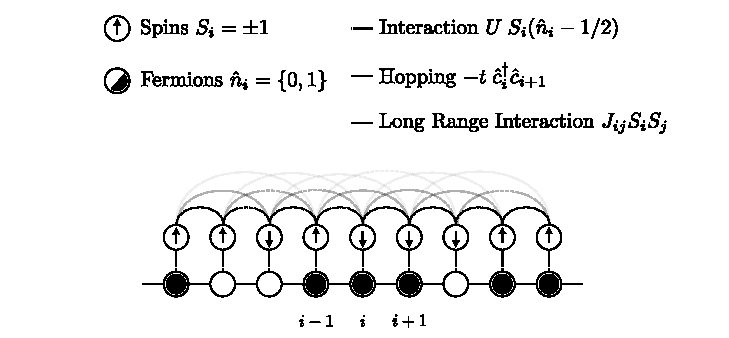
\includegraphics[width=1\textwidth,height=\textheight]{figure_code/intro_chapter/lrfk_schematic}
\caption[{Falicov-Kimball Model Diagram}]{The Long Range Falicov-Kimball (LRFK) Model is a model of classical spins \(S_i\) coupled to spinless fermions \(\hat{c}_i\) where the fermions are mobile with hopping \(t\) and the fermions are coupled to the spins by an Ising type interaction with strength \(U\). The difference from the standard FK model is the presence of a long range interaction between the spins \(J_{ij}S_i S_j\).}
\label{fig:lrfk_schematic}
\end{figure}
}

Dimensionality is crucial for the physics of both localisation and phase transitions. We have already seen that the one dimensional standard FK model cannot support an ordered phase at finite temperatures and therefore has no finite temperature phase transition (FTPT).

On bipartite lattices in dimensions 2 and above the FK model exhibits a finite temperature phase transition to an ordered charge density wave (CDW) phase~\autocite{maskaThermodynamicsTwodimensionalFalicovKimball2006}. In this phase, the spins order anti-ferromagnetically, breaking the \(\mathbb{Z}_2\) symmetry. In 1D, however, Periel's argument~\autocite{peierlsIsingModelFerromagnetism1936,kennedyItinerantElectronModel1986} states that domain walls only introduce a constant energy penalty into the free energy while bringing a entropic contribution logarithmic in system size. Hence the 1D model does not have a finite temperature phase transition. However 1D systems are much easier to study numerically and admit simpler realisations experimentally. We therefore introduce a long-range coupling between the ions in order to stabilise a CDW phase in 1D.

We interpret the FK model as a model of spinless fermions, \(c^\dagger_{i}\), hopping on a 1D lattice against a classical Ising spin background, \(S_i \in {\pm \frac{1}{2}}\). The fermions couple to the spins via an onsite interaction with strength \(U\) which we supplement by a long-range interaction, \[
J_{ij} = 4\kappa J\; (-1)^{|i-j|} |i-j|^{-\alpha},
\]

between the spins. The additional coupling is very similar to that of the long range Ising model, it stabilises the Antiferromagnetic (AFM) order of the Ising spins which promotes the finite temperature CDW phase of the fermionic sector.

The hopping strength of the electrons, \(t = 1\), sets the overall energy scale and we concentrate throughout on the particle-hole symmetric point at zero chemical potential and half filling~\autocite{gruberFalicovKimballModelReview1996}.

\[\begin{aligned}
H_{\mathrm{FK}} = & \;U \sum_{i} S_i\;(c^\dagger_{i}c_{i} - \tfrac{1}{2}) -\;t \sum_{i} (c^\dagger_{i}c_{i+1} + \textit{h.c.)}\\ 
 &  + \sum_{i, j}^{N} J_{ij}  S_i S_j
\label{eq:HFK}\end{aligned}\]

Without proper normalisation, the long range coupling would render the critical temperature strongly system size dependent for small system sizes. Within a mean field approximation the critical temperature scales with the effective coupling to all the neighbours of each site, which for a system with \(N\) sites is \(\sum_{i=1}^{N} i^{-\alpha}\). Hence, the normalisation \(\kappa^{-1} = \sum_{i=1}^{N} i^{-\alpha}\), renders the critical temperature independent of system size in the mean field approximation. This greatly improves the finite size behaviour of the model.

Taking the limit \(U = 0\) decouples the spins from the fermions, which gives a spin sector governed by a classical LRI model. Note, the transformation of the spins \(S_i \to (-1)^{i} S_i\) maps the AFM model to the FM one. As discussed in the background section, Peierls' classic argument can be extended to long range couplings to show that, for the 1D LRI model, a power law decay of \(\alpha < 2\) is required for a FTPT as the energy of defect domain then scales with the system size and can overcome the entropic contribution. A renormalisation group analysis supports this finding and shows that the critical exponents are only universal for \(\alpha \leq 3/2\)~\autocite{ruelleStatisticalMechanicsOnedimensional1968,thoulessLongRangeOrderOneDimensional1969,angeliniRelationsShortrangeLongrange2014}. In the following, we choose \(\alpha = 5/4\) to avoid the additional complexity of non-universal critical points.

\hypertarget{sec:lrfk-methods}{%
\section{Methods}\label{sec:lrfk-methods}}

To evaluate thermodynamic averages, I perform classical Markov Chain Monte Carlo random walks over the space of spin configurations of the LRFK model, at each step diagonalising the effective electronic Hamiltonian~\autocite{maskaThermodynamicsTwodimensionalFalicovKimball2006}. Using a Binder-cumulant method~\autocite{binderFiniteSizeScaling1981,musialMonteCarloSimulations2002}, I demonstrate that the model has a finite temperature phase transition when the interaction is sufficiently long-ranged. In this section I will discuss the thermodynamics of the model and how they are amenable to an exact Markov Chain Monte Carlo method.

\hypertarget{thermodynamics-of-the-lrfk-model}{%
\subsection{Thermodynamics of the LRFK Model}\label{thermodynamics-of-the-lrfk-model}}

\hypertarget{fig:raw_steps_single_flip}{%
\begin{figure}
\centering
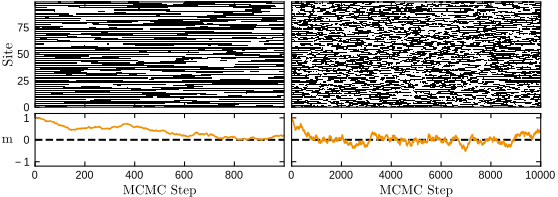
\includegraphics[width=1\textwidth,height=\textheight]{figure_code/fk_chapter/raw_steps_single_flip}
\caption[{Comparison of different proposal distributions}]{Two Markov Chain Monte Carlo (MCMC) walks starting from the CDW state for a system with \(N = 100\) sites and 10,000 MCMC steps but at a temperature close to but above the ordered state (left column) and much higher than it (right column). In this simulation, only a single spin can be flipped per step according to the Metropolis-Hastings Algorithm. The staggered magnetisation \(m = N^{-1} \sum_i (-1)^i \; S_i\) order parameter is plotted below. At both temperatures the thermal average of \(m\) is zero, while the initial state has \(m = 1\). The higher temperature allows the MCMC to converge more quickly and to fluctuate about the mean with a shorter autocorrelation time. \(t = 1, \alpha = 1.25, T = {2.5,5}, J = U = 5\)}
\label{fig:raw_steps_single_flip}
\end{figure}
}

A classical Markov Chain Monte Carlo (MCMC) method allows us to solve our LRFK model efficiently, yielding unbiased estimates of thermal expectation values, see \cref{fig:raw_steps_single_flip}.

Since the spin configurations are classical, the LRFK Hamiltonian can be split into a classical spin part \(H_s\) and an operator valued part \(H_c\).

\[\begin{aligned}
H_s& = - \frac{U}{2}S_i + \sum_{i, j}^{N} J_{ij} S_i S_j \\
H_c& = \sum_i U S_i c^\dagger_{i}c^{\phantom{\dagger}}_{i} -t(c^\dagger_{i}c^{\phantom{\dagger}}_{i+1} + c^\dagger_{i+1}c^{\phantom{\dagger}}_{i}). \end{aligned}\]

The partition function can then be written as a sum over spin configurations, \(\vec{S} = (S_0, S_1...S_{N-1})\):

\[\begin{aligned}
\mathcal{Z} = \mathrm{Tr} e^{-\beta H}= \sum_{\vec{S}} e^{-\beta H_s} \mathrm{Tr}_c e^{-\beta H_c} .\end{aligned}\]

The contribution of \(H_c\) to the grand canonical partition function can be obtained by performing the sum over eigenstate occupation numbers giving \(-\beta F_c[\vec{S}] = \sum_k \ln{(1 + e^{- \beta \epsilon_k})}\) where \({\epsilon_k[\vec{S}]}\) are the eigenvalues of the matrix representation of \(H_c\) determined through exact diagonalisation. This gives a partition function containing a classical energy which corresponds to the long-range interaction of the spins, and a free energy which corresponds to the quantum subsystem

\[\begin{aligned}
\mathcal{Z} = \sum_{\vec{S}} e^{-\beta H_S[\vec{S}] - \beta F_c[\vec{S}]} = \sum_{\vec{S}} e^{-\beta E[\vec{S}]}.\end{aligned}\]

\hypertarget{markov-chain-monte-carlo-and-emergent-disorder}{%
\subsection{Markov Chain Monte Carlo and Emergent Disorder}\label{markov-chain-monte-carlo-and-emergent-disorder}}

Classical MCMC defines a weighted random walk over the spin states \((\vec{S}_0, \vec{S}_1, \vec{S}_2, ...)\), such that the likelihood of visiting a particular state converges to its Boltzmann probability \(p(\vec{S}) = \mathcal{Z}^{-1} e^{-\beta E}\). Hence, any observable can be estimated as a mean over the states visited by the walk~\autocite{binderGuidePracticalWork1988,kerteszAdvancesComputerSimulation1998,wolffMonteCarloErrors2004},

\[\begin{aligned}
\label{eq:thermal_expectation}
\langle O \rangle & = \sum_{\vec{S}} p(\vec{S}) \langle O \rangle_{\vec{S}}\\
                  & = \sum_{i = 0}^{M} \langle O\rangle_{\vec{S}_i} \pm \mathcal{O}(M^{-\tfrac{1}{2}}),
\end{aligned}\]

where the former sum runs over the entire state space while the latter runs over all the states visited by a particular MCMC run,

\[\begin{aligned}
\langle O \rangle_{\vec{S}}& = \sum_{\nu} n_F(\epsilon_{\nu}) \langle O \rangle{\nu},
\end{aligned}\]

where \(\nu\) runs over the eigenstates of \(H_c\) for a particular spin configuration and \(n_F(\epsilon) = \left(e^{-\beta\epsilon} + 1\right)^{-1}\) is the Fermi function.

The choice of the transition function for MCMC is under-determined as one only needs to satisfy a set of balance conditions for which there are many solutions~\autocite{kellyReversibilityStochasticNetworks1981}. Here, we incorporate a modification to the standard Metropolis-Hastings algorithm~\autocite{hastingsMonteCarloSampling1970} gleaned from Krauth~\autocite{krauthIntroductionMonteCarlo1998}.

The standard algorithm decomposes the transition probability into \(\mathcal{T}(a \to b) = p(a \to b)\mathcal{A}(a \to b)\). Here, \(p\) is the proposal distribution, that we can directly sample from, while \(\mathcal{A}\) is the acceptance probability. The standard Metropolis-Hastings choice is

\[\mathcal{A}(a \to b) = \min\left(1, \frac{p(b\to a)}{p(a\to b)} e^{-\beta \Delta E}\right)\;,\]

with \(\Delta E = E_b - E_a\). The walk then proceeds by sampling a state \(b\) from \(p\) and moving to \(b\) with probability \(\mathcal{A}(a \to b)\). The latter operation is typically implemented by performing a transition if a uniform random sample from the unit interval is less than \(\mathcal{A}(a \to b)\) and otherwise repeating the current state as the next step in the random walk. The proposal distribution is often symmetric, so it does not appear in \(\mathcal{A}\). Here, we flip a small number of sites in \(b\) at random to generate proposals, which is a symmetric proposal.

In our computations~\autocite{hodsonMCMCFKModel2021}, we employ a modification to this algorithm based on the observation that the free energy of the FK system is composed of a classical part which is much quicker to compute than the quantum part. Hence, we can obtain a computational speed up by first considering the value of the classical energy difference \(\Delta H_s\) and rejecting the transition if the former is too high. We only compute the quantum energy difference \(\Delta F_c\) if the transition is accepted. We then perform a second rejection sampling step based upon it. This corresponds to two nested comparisons with the majority of the work only occurring if the first test passes. This modified scheme has the acceptance function

\[\mathcal{A}(a \to b) = \min\left(1, e^{-\beta \Delta H_s}\right)\min\left(1, e^{-\beta \Delta F_c}\right).\]

For the model parameters used, we find that with our new scheme the matrix diagonalisation is skipped around 30\% of the time at \(T = 2.5\) and up to 80\% at \(T = 1.5\). We observe that for \(N = 50\), the matrix diagonalisation, if it occurs, occupies around 60\% of the total computation time for a single step. This rises to 90\% at N = 300 and further increases for larger N. We therefore get the greatest speedup for large system sizes at low temperature where many prospective transitions are rejected at the classical stage and the matrix computation takes up the greatest fraction of the total computation time. The upshot is that we find a speedup of up to a factor of 10 at the cost of very little extra algorithmic complexity.

Our two-step method should be distinguished from the more common method for speeding up MCMC, which is to add asymmetry to the proposal distribution to make it as similar as possible to \(\min\left(1, e^{-\beta \Delta E}\right)\). This reduces the number of rejected states, which brings the algorithm closer in efficiency to a direct sampling method. However, it comes at the expense of requiring a way to directly sample from this complex distribution. This is a problem which MCMC was employed to solve in the first place. For example, recent work trains restricted Boltzmann machines (RBMs) to generate samples for the proposal distribution of the FK model~\autocite{huangAcceleratedMonteCarlo2017}. The RBMs are chosen as a parametrisation of the proposal distribution that can be efficiently sampled from, while offering sufficient flexibility that they can be adjusted to match the target distribution. Our proposed method is considerably simpler and does not require training while still reaping some of the benefits of reduced computation.

\hypertarget{scaling}{%
\subsection{Scaling}\label{scaling}}

\hypertarget{fig:binder_cumulants}{%
\begin{figure}
\centering
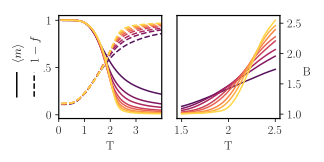
\includegraphics[width=1\textwidth,height=\textheight]{figure_code/fk_chapter/binder_cumulants/binder_cumulants}
\caption[{Binder Cumulants}]{(Left) The order parameters, \(\langle m^2 \rangle\) (solid) and \(1 - f\) (dashed) describing the onset of the charge density wave phase of the LRFK model at low temperature with staggered magnetisation \(m = N^{-1} \sum_i (-1)^i S_i\) and fermionic order parameter \(f = 2 N^{-1}|\sum_i (-1)^i \; \langle c^\dagger_{i}c^{\phantom{\dagger}}_{i}| \rangle\) . (Right) The crossing of the Binder cumulant, \(B = \langle m^4 \rangle / \langle m^2 \rangle^2\), with system size provides a diagnostic that the phase transition is not a finite size effect, it is used to estimate the critical lines shown in the phase diagram later. All plots use system sizes \(N = [10,20,30,50,70,110,160,250]\) and lines are coloured from \(N = 10\) in dark blue to \(N = 250\) in yellow. The parameter values \(U = 5,\;J = 5,\;\alpha = 1.25\) except where explicitly mentioned.}
\label{fig:binder_cumulants}
\end{figure}
}

To improve the scaling of finite size effects, we make the replacement \(|i - j|^{-\alpha} \rightarrow |f(i - j)|^{-\alpha}\), in both \(J_{ij}\) and \(\kappa\), where \(f(x) = \frac{N}{\pi}\sin \frac{\pi x}{N}\). \(f\) is smooth across the circular boundary and its effect diminished for larger systems~\autocite{fukuiOrderNClusterMonte2009}. We only consider even system sizes given that odd system sizes are not commensurate with a CDW state.

To identify critical points, I use the Binder cumulant \(U_B\) defined by

\[
U_B = 1 - \frac{\langle\mu_4\rangle}{3\langle\mu_2\rangle^2},
\]

where \(\mu_n = \langle(m - \langle m\rangle)^n\rangle\) are the central moments of the order parameter \(m = \sum_i (-1)^i (2n_i - 1) / N\). The Binder cumulant evaluated against temperature is a diagnostic for the existence of a phase transition. If multiple such curves are plotted for different system sizes, a crossing indicates the location of a critical point while the lines do not cross for systems that don't have a phase transition in the thermodynamic limit~\autocite{binderFiniteSizeScaling1981,musialMonteCarloSimulations2002}.

\hypertarget{sec:lrfk-results}{%
\section{Results}\label{sec:lrfk-results}}

Looking at the results of our MCMC simulations, we find a rich phase diagram with a CDW FTPT and interaction-tuned Anderson versus Mott localized phases similar to the 2D FK model~\autocite{antipovInteractionTunedAndersonMott2016}. We explore the localization properties of the fermionic sector and find that the localisation lengths vary dramatically across the phases and for different energies. Although moderate system sizes indicate the coexistence of localized and delocalized states within the CDW phase, we find quantitatively similar behaviour in a model of uncorrelated binary disorder on a CDW background. For large system sizes, i.e.~for our 1D disorder model we can treat linear sizes of several thousand sites, we find that all states are eventually localized with a localization length which diverges towards zero temperature.

\hypertarget{fig:phase-diagram-lrfk}{%
\begin{figure}
\centering
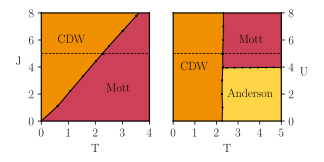
\includegraphics[width=1\textwidth,height=\textheight]{figure_code/fk_chapter/phase_diagram/phase_diagram}
\caption[{Long Range Falicov Kimball Model Phase Diagram}]{Phase diagrams of the long-range 1D FK model. (Left) The TJ plane at \(U = 5\): the CDW ordered phase is separated from a disordered Mott insulating phase by a critical temperature \(T_c\), linear in J. (Right) The TU plane at \(J = 5\): the disordered phase is split into two: at large/small U there's a MI/Anderson phase characterised by the presence/absence of a gap at \(E=0\) in the single particle energy spectrum. \(U_c\) is independent of temperature. At \(U = 0\) the fermions are decoupled from the spins forming a simple Fermi gas.}
\label{fig:phase-diagram-lrfk}
\end{figure}
}

\hypertarget{lrfk-results-phase-diagram}{%
\subsection{Phase Diagram}\label{lrfk-results-phase-diagram}}

Using the MCMC methods described in the previous section I will now discuss the results of extensive MCMC simulations of the model, starting with the phase diagram in the fermion spin coupling \(U\), the strength of the long range spin-spin coupling \(J\) and the temperature \(T\).

\Cref{fig:phase-diagram-lrfk} shows the phase diagram for constant \(U=5\) and constant \(J=5\), respectively. The transition temperatures were determined from the crossings of the Binder cumulants \(B_4 = \langle m^4 \rangle /\langle m^2 \rangle^2\)~\autocite{binderFiniteSizeScaling1981}.

The CDW transition temperature is largely independent from the strength of the interaction \(U\). This demonstrates that the phase transition is driven by the long-range term \(J\) with little effect from the coupling to the fermions \(U\). The physics of the spin sector in the long-range FK model mimics that of the long range Ising (LRI) model and is not significantly altered by the presence of the fermions. In two dimensions the transition to the CDW phase is mediated by an RKYY-like interaction~\autocite{rusinCalculationRKKYRange2017} but this is insufficient to stabilise long range order in one dimension. That the critical temperature \(T_c\) does not depend on \(U\) in our model further confirms this.

The main order parameters for this model is the staggered magnetisation \(m = N^{-1} \sum_i (-1)^i S_i\) that signals the onset of a charge density wave (CDW) phase at low temperature. However, my main interest concerns the additional structure of the fermionic sector in the high temperature phase. Following Ref.~\autocite{antipovInteractionTunedAndersonMott2016}, we can distinguish between the Mott and Anderson insulating phases. The Mott insulator is characterised by a gapped DOS in the absence of a CDW, instead the gap is driven entirely by interaction effect. Thus, the opening of a gap for large \(U\) is distinct from the gap-opening induced by the translational symmetry breaking in the CDW state below \(T_c\). The Anderson phase is gapless but, as we explain below, shows localised fermionic eigenstates hence it also has insulating character.

\hypertarget{localisation-properties}{%
\subsection{Localisation Properties}\label{localisation-properties}}

\hypertarget{fig:DOS}{%
\begin{figure}
\centering
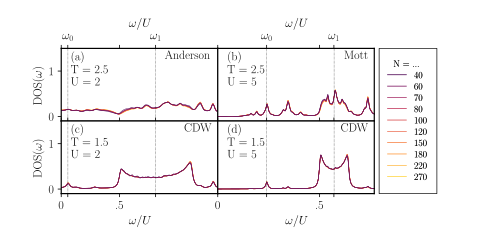
\includegraphics[width=1\textwidth,height=\textheight]{figure_code/fk_chapter/DOS/DOS}
\caption[{Energy resolved DOS(\(\omega\)) in the difference phases.}]{Energy resolved DOS(\(\omega\)) against system size \(N\) in all three phases. The charge density wave phase is shown in both the high and low \(U\) regime for completeness. The top left panel shows the Anderson phase at \(U = 2\) and high \(T = 2.5\), this phase is gapless but does not conduct due to Anderson localisation. In the lower left pane at \(U = 2\) and low \(T = 1.5\), charge density wave order sets in, allowing the single particle eigenstates to become extended but opening a gap in their band structure. In the upper right panel at \(U = 5\) and high \(T = 2.5\) the states are localised by disorder and an interaction driven gap opens, a Mott insulator. Finally the charge density wave phase at \(U = 5\) and \(T = 1.5\) is qualitatively similar to the lower left panel except that the gap scales with \(U\). For all the plots \(J = 5,\;\alpha = 1.25\).}
\label{fig:DOS}
\end{figure}
}

The MCMC formulation suggests viewing the spin configurations as a form of annealed binary disorder whose probability distribution is given by the Boltzmann weight \(e^{-\beta H_S[\vec{S}] - \beta F_c[\vec{S}]}\). This makes apparent the link to the study of disordered systems and Anderson localisation. While these systems are typically studied by defining the probability distribution for the quenched disorder potential externally, here we have a translation invariant system with disorder as a natural consequence of the Ising background field conserved under the dynamics.

In the limits of zero and infinite temperature, our model becomes a simple tight-binding model for the fermions. At zero temperature, the spin background is in one of the two translation invariant AFM ground states with two gapped fermionic CDW bands at energies

\[E_{\pm} = \pm\sqrt{\frac{1}{4}U^2 + 2t^2(1 + \cos ka)^2}\;.\]

At infinite temperature, all the spin configurations become equally likely and the fermionic model reduces to one of binary uncorrelated disorder in which all eigenstates are Anderson localised~\autocite{abrahamsScalingTheoryLocalization1979}. An Anderson localised state centered around \(r_0\) has magnitude that drops exponentially over some localisation length \(\xi\) i.e \(|\psi(r)|^2 \sim \exp{-|r - r_0|/\xi}\). Calculating \(\xi\) directly is numerically demanding. Therefore, we determine if a given state is localised via the energy-resolved IPR and the DOS defined as

\[\begin{aligned}
\mathrm{DOS}(\vec{S}, \omega)& = N^{-1} \sum_{i} \delta(\epsilon_i - \omega)\\
\mathrm{IPR}(\vec{S}, \omega)& = \; N^{-1} \mathrm{DOS}(\vec{S}, \omega)^{-1} \sum_{i,j} \delta(\epsilon_i - \omega)\;\psi^{4}_{i,j}\end{aligned}\]

where \(\epsilon_i\) and \(\psi_{i,j}\) are the \(i\)th energy level and \(j\)th element of the corresponding eigenfunction, both dependent on the background spin configuration \(\vec{S}\).

\hypertarget{fig:IPR_scaling}{%
\begin{figure}
\centering
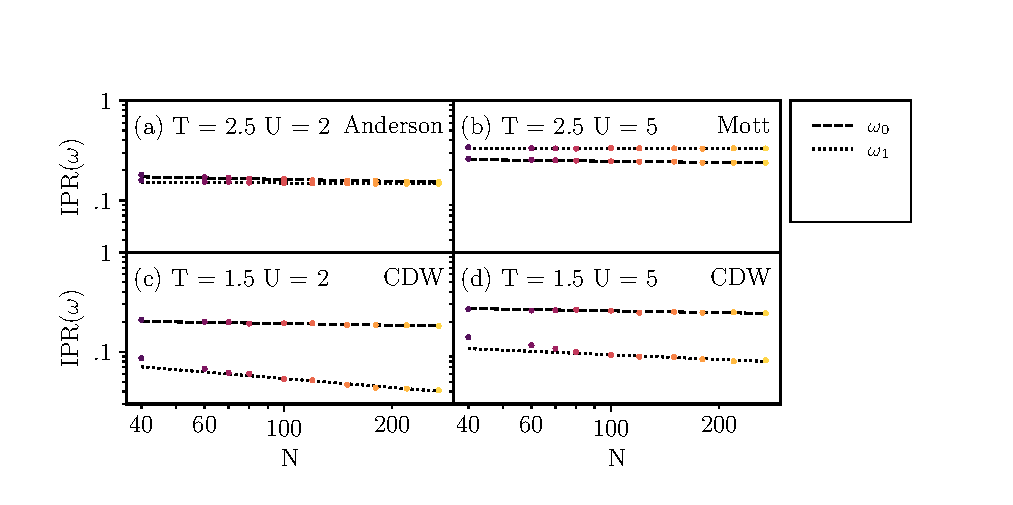
\includegraphics[width=1\textwidth,height=\textheight]{figure_code/fk_chapter/DOS/IPR_scaling}
\caption[{Scaling of IPR(\(\omega\)) against system size \(N\).}]{The IPR(\(\omega\)) scaling with \(N\) at fixed energy for each phase and for points both in the gap (\(\omega_0\)) and in a band (\(\omega_1\)). The slope of the line yields the scaling exponent \(\tau\) defined by \(\mathrm{IPR} \propto N^{-\tau}\)). \(\tau\) close to zero implies that the states at that energy are localised while \(\tau = -d\) corresponds to extended states where \(d\) is the system dimension. All but the bands of the charge density wave phase are approximately localised with \(\tau\) is very close to zero. The bands in the charge density wave phase are localised with long localisation lengths at finite temperatures that extend to infinity as the temperature approaches zero. For all the plots \(J = 5,\;\alpha = 1.25\). The measured \(\tau_0,\tau_1\) for each figure are: (a) \((0.06\pm0.01, 0.02\pm0.01\) (b) \(0.04\pm0.02, 0.00\pm0.01\) (c) \(0.05\pm0.03, 0.30\pm0.03\) (d) \(0.06\pm0.04, 0.15\pm0.05\) We show later that the apparent slight scaling of the IPR with system size in the localised cases can be explained by finite size effects due to the changing defect density with system size rather than due to delocalisation of the states.}
\label{fig:IPR_scaling}
\end{figure}
}

The scaling of the IPR with system size \(\mathrm{IPR} \propto N^{-\tau}\) depends on the localisation properties of states at that energy. For delocalised states, e.g.~Bloch waves, \(\tau\) is the physical dimension. For fully localised states \(\tau\) goes to zero in the thermodynamic limit. However, for special types of disorder such as binary disorder, the localisation lengths can be large comparable to the system size at hand, which can make it difficult to extract the correct scaling. An additional complication arises from the fact that the scaling exponent may display intermediate behaviours for correlated disorder and in the vicinity of a localisation-delocalisation transition~\autocite{kramerLocalizationTheoryExperiment1993,eversAndersonTransitions2008}. The thermal defects of the CDW phase lead to a binary disorder potential with a finite correlation length, which in principle could result in delocalized eigenstates.

The key question for our system is then: How is the \(T=0\) CDW phase with fully delocalized fermionic states connected to the fully localized phase at high temperatures?

For a representative set of parameters covering all three phases \cref{fig:DOS} shows the density of states as function of energy while \cref{fig:IPR_scaling}~shows \(\tau\), the scaling exponent of the IPR with system size, The DOS is symmetric about \(0\) because of the particle hole symmetry of the model. At high temperatures, all of the eigenstates are localised in both the Mott and Anderson phases (with \(\tau \leq 0.07\) for our system sizes). We also checked that the states are localised by direct inspection. Note that there are in-gap states for instance at \(\omega_0\), below the upper band which are localized and smoothly connected across the phase transition.

\hypertarget{fig:gap_opening_U5}{%
\begin{figure}
\centering
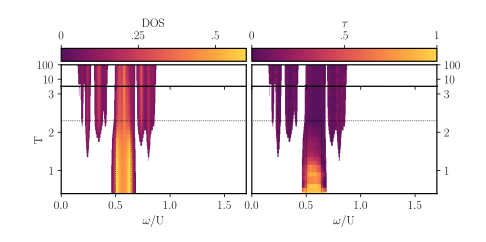
\includegraphics[width=1\textwidth,height=\textheight]{figure_code/fk_chapter/gap_opening/gap_opening_U5}
\caption[{The transition from CDW to the Mott phase}]{The DOS (a) and scaling exponent \(\tau\) (b) as a function of energy for the CDW to gapped Mott phase transition at \(U=5\). Regions where the DOS is close to zero are shown in white. The scaling exponent \(\tau\) is obtained from fits to \(IPR(N) = A N^{-\lambda}\) for a range of system sizes. \(J = 5,\;\alpha = 1.25\)}
\label{fig:gap_opening_U5}
\end{figure}
}

In the CDW phases at \(U=2\) and \(U=5\), we find for the states within the gapped CDW bands, e.g.~at \(\omega_1\), scaling exponents \(\tau = 0.30\pm0.03\) and \(\tau = 0.15\pm0.05\), respectively. This surprising finding suggests that the CDW bands are partially delocalised with multi-fractal behaviour of the wavefunctions~\autocite{eversAndersonTransitions2008}. This phenomenon would be unexpected in a 1D model as they generally do not support delocalisation in the presence of disorder except as the result of correlations in the emergent disorder potential~\autocite{croyAndersonLocalization1D2011,goldshteinPurePointSpectrum1977}. However, we later show by comparison to an uncorrelated Anderson model that these nonzero exponents are a finite size effect and the states are localised with a finite \(\xi\) similar to the system size, an example of weak localisation. As a result, the IPR does not scale correctly until the system size has grown much larger than \(\xi\). \cref{fig:DM_IPR_scaling} shows that the scaling of the IPR in the CDW phase does flatten out eventually.

Next, we use the DOS and the scaling exponent \(\tau\) to explore the localisation properties over the energy-temperature plane in \cref{fig:gap_opening_U2} and \cref{fig:gap_opening_U5}. Gapped areas are shown in white, which highlights the distinction between the gapped Mott phase and the ungapped Anderson phase. In-gap states appear just below the critical point, smoothly filling the bandgap in the Anderson phase and forming islands in the Mott phase. As in the finite~\autocite{zondaGaplessRegimeCharge2019} and infinite dimensional~\autocite{hassanSpectralPropertiesChargedensitywave2007} cases, the in-gap states merge and are pushed to lower energy for decreasing U as the \(T=0\) CDW gap closes. Intuitively, the presence of in-gap states can be understood as a result of domain wall fluctuations away from the AFM ordered background. These domain walls act as local potentials for impurity-like bound states~\autocite{zondaGaplessRegimeCharge2019}.

\hypertarget{fig:gap_opening_U2}{%
\begin{figure}
\centering
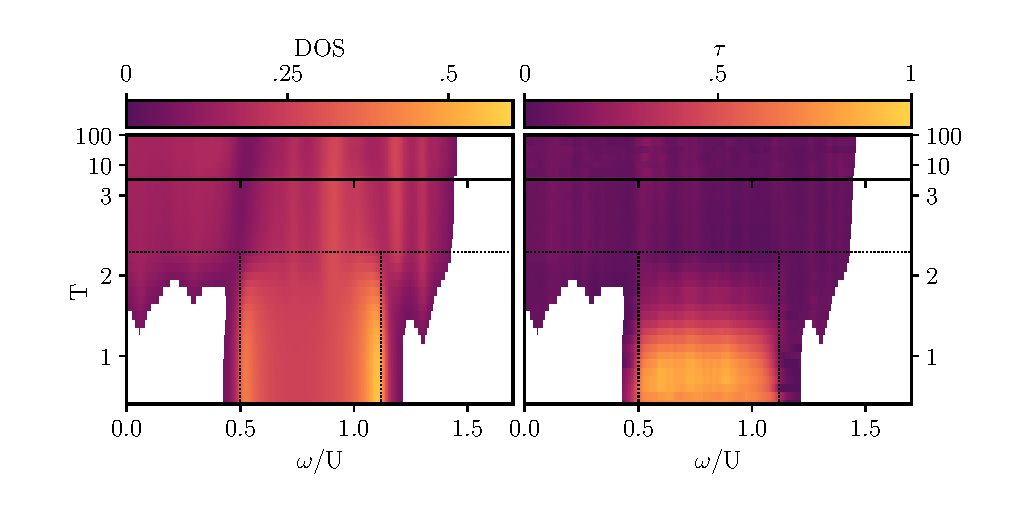
\includegraphics[width=1\textwidth,height=\textheight]{figure_code/fk_chapter/gap_opening/gap_opening_U2}
\caption[{The transition from CDW to the Anderson Phase}]{The DOS (a) and scaling exponent \(\tau\) (b) as a function of energy for the CDW phase to the gapless Anderson insulating phase at \(U=2\). Regions where the DOS is close to zero are shown in white. The scaling exponent \(\tau\) is obtained from fits to \(IPR(N) = A N^{-\lambda}\) for a range of system sizes. \(J = 5,\;\alpha = 1.25\)}
\label{fig:gap_opening_U2}
\end{figure}
}

In order to understand the localization properties we can compare the behaviour of our model with that of a simpler Anderson disorder model (DM) in which the spins are replaced by a CDW background with uncorrelated binary defect potentials. This is defined by replacing the spin degree of freedom in the FK model \(S_i = \pm \tfrac{1}{2}\) with a disorder potential \(d_i = \pm \tfrac{1}{2}\) controlled by a defect density \(\rho\) such that \(d_i = -\tfrac{1}{2}\) with probability \(\rho/2\) and \(d_i = \tfrac{1}{2}\) otherwise. \(\rho/2\) is used rather than \(\rho\) so that the disorder potential takes on the zero temperature CDW ground state at \(\rho = 0\) and becomes a random choice over spin states at \(\rho = 1\) i.e the infinite temperature limit.

\[\begin{aligned}
H_{\mathrm{DM}} = & \;U \sum_{i} (-1)^i \; d_i \;(c^\dagger_{i}c_{i} - \tfrac{1}{2}) \\
& -\;t \sum_{i} c^\dagger_{i}c_{i+1} + c^\dagger_{i+1}c_{i}
\end{aligned}\]

\cref{fig:DM_DOS} and \cref{fig:DM_IPR_scaling} compare the FK model to the disorder model at different system sizes, matching the defect densities of the disorder model to the FK model at \(N = 270\) above and below the CDW transition. We find very good, even quantitative, agreement between the FK and disorder models, which suggests that correlations in the spin sector do not play a significant role.

\hypertarget{fig:DM_DOS}{%
\begin{figure}
\centering
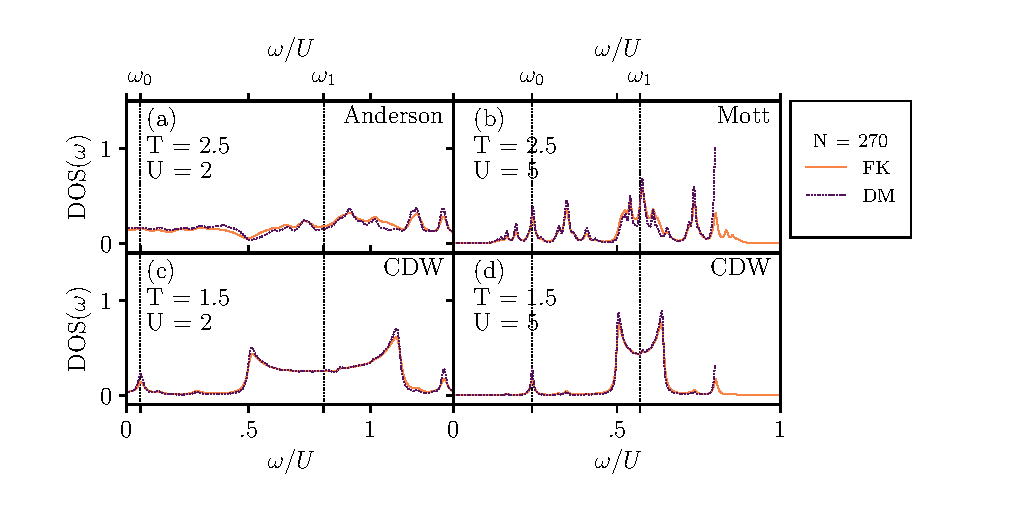
\includegraphics[width=1\textwidth,height=\textheight]{figure_code/fk_chapter/disorder_model/DM_DOS}
\caption[{FK model compared to binary disorder model: DOS}]{A comparison of the full FK model to a simple binary disorder model (DM) with a CDW wave background perturbed by uncorrelated defects at density \(0 < \rho < 1\) matched to the \(\rho\) for the largest corresponding FK model. As in \cref{fig:DOS}, the Energy resolved DOS(\(\omega\)) is shown. The DOSs match well implying that correlations in the CDW wave fluctuations are not relevant at these system parameters.}
\label{fig:DM_DOS}
\end{figure}
}

As we can sample directly from the disorder model, rather than through MCMC, the samples are uncorrelated. Hence we can evaluate much larger system sizes with the disorder model which enables us to pin down the correct localisation effects. In particular, what appear to be delocalized states for small system sizes eventually turn out to be states with large localization length. The localization length diverges towards the ordered zero temperature CDW state. The interplay of interactions, which here produce as peculiar binary potential, and localization can be very intricate and the added advantage of a 1D model is that we can explore very large system sizes.

\hypertarget{fig:DM_IPR_scaling}{%
\begin{figure}
\centering
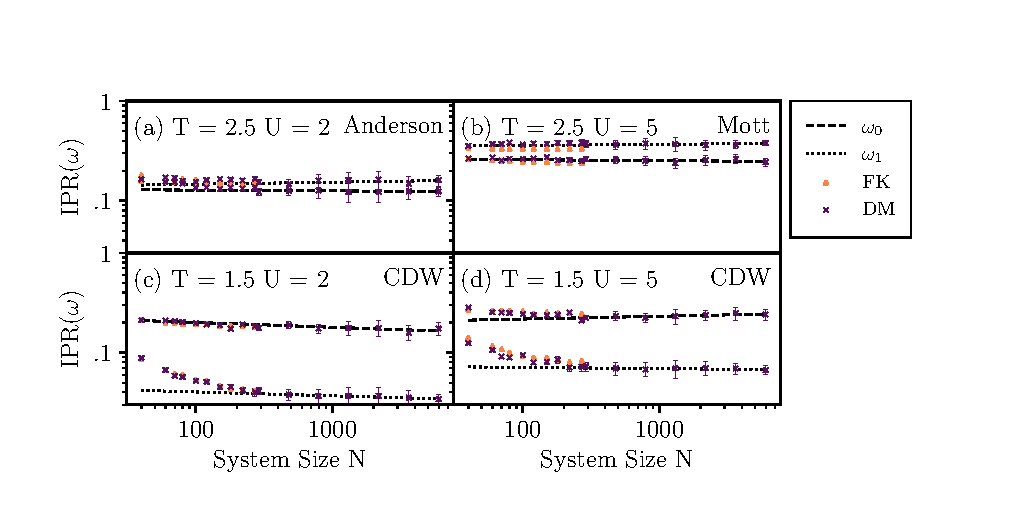
\includegraphics[width=1\textwidth,height=\textheight]{figure_code/fk_chapter/disorder_model/DM_IPR_scaling}
\caption[{FK model compared to binary disorder model: IPR Scaling}]{A comparison of the full FK model to a simple binary disorder model (DM) with a CDW wave background perturbed by uncorrelated defects at density \(0 < \rho < 1\) matched to the \(\rho\) for the largest corresponding FK model. As in \cref{fig:IPR_scaling} \(\tau(\omega)\) the scaling of IPR(\(\omega\)) with system size, , is shown both in gap (\(\omega_0\)) and in the band (\(\omega_1\)). This data makes clear that the apparent scaling of IPR with system size at small sysis a finite size effect due to weak localisation~\autocite{antipovInteractionTunedAndersonMott2016}, hence all the states are indeed localised as one would expect in 1D. The disorder model \(\tau_0,\tau_1\) for each figure are: (a) \(0.01\pm0.05, -0.02\pm0.06\) (b) \(0.01\pm0.04, -0.01\pm0.04\) (c) \(0.05\pm0.06, 0.04\pm0.06\) (d) \(-0.03\pm0.06, 0.01\pm0.06\). The lines are fit on system sizes \(N > 400\)}
\label{fig:DM_IPR_scaling}
\end{figure}
}

\hypertarget{fk-conclusion}{%
\section{Discussion and Conclusion}\label{fk-conclusion}}

The FK model is one of the simplest non-trivial models of interacting fermions. We studied its thermodynamic and localisation properties brought down in dimensionality to one dimension by adding a novel long-ranged coupling designed to stabilise the CDW phase present in dimension two and above.

Our MCMC approach emphasises the presence of a disorder-free localization mechanism within our translationally invariant system. Further, it gives a significant speed up over the naive method. We show that our LRFK model retains much of the rich phase diagram of its higher dimensional cousins. Careful scaling analysis indicates that all the single particle eigenstates eventually localise at non-zero temperature albeit only for very large system sizes of several thousand.

Our work raises a number of interesting questions for future research. A straightforward but numerically challenging problem is to pin down the model's behaviour closer to the critical point where correlations in the spin sector would become significant. Would this modify the localisation behaviour? Similar to other soluble models of disorder-free localisation, we expect intriguing out-of equilibrium physics, for example slow entanglement dynamics akin to more generic interacting systems~\autocite{hartLogarithmicEntanglementGrowth2020}. One could also investigate whether the rich ground state phenomenology of the FK model as a function of filling~\autocite{gruberGroundStatesSpinless1990} such as the devil's staircase~\autocite{michelettiCompleteDevilTextquotesingles1997} as well as superconductor like states~\autocite{caiVisualizingEvolutionMott2016} could be stabilised at finite temperature.

In a broader context, we envisage that long-range interactions can also be used to gain a deeper understanding of the temperature evolution of topological phases. One example would be a long-ranged FK version of the celebrated Su-Schrieffer-Heeger model where one could explore the interplay of topological bound states and thermal domain wall defects. Finally, the rich physics of our model should be realizable in systems with long-range interactions, such as trapped ion quantum simulators, where one can also explore the fully interacting regime with a dynamical background field.

\printbibliography[heading=subbibintoc]
\end{refsection}

\hypertarget{chap:4-the-amorphous-kitaev-model}{\chapter{The Amorphous Kitaev Honeycomb Model}}
\backgroundsetup{scale = 1, angle = 0, opacity = 0.5,
  contents = {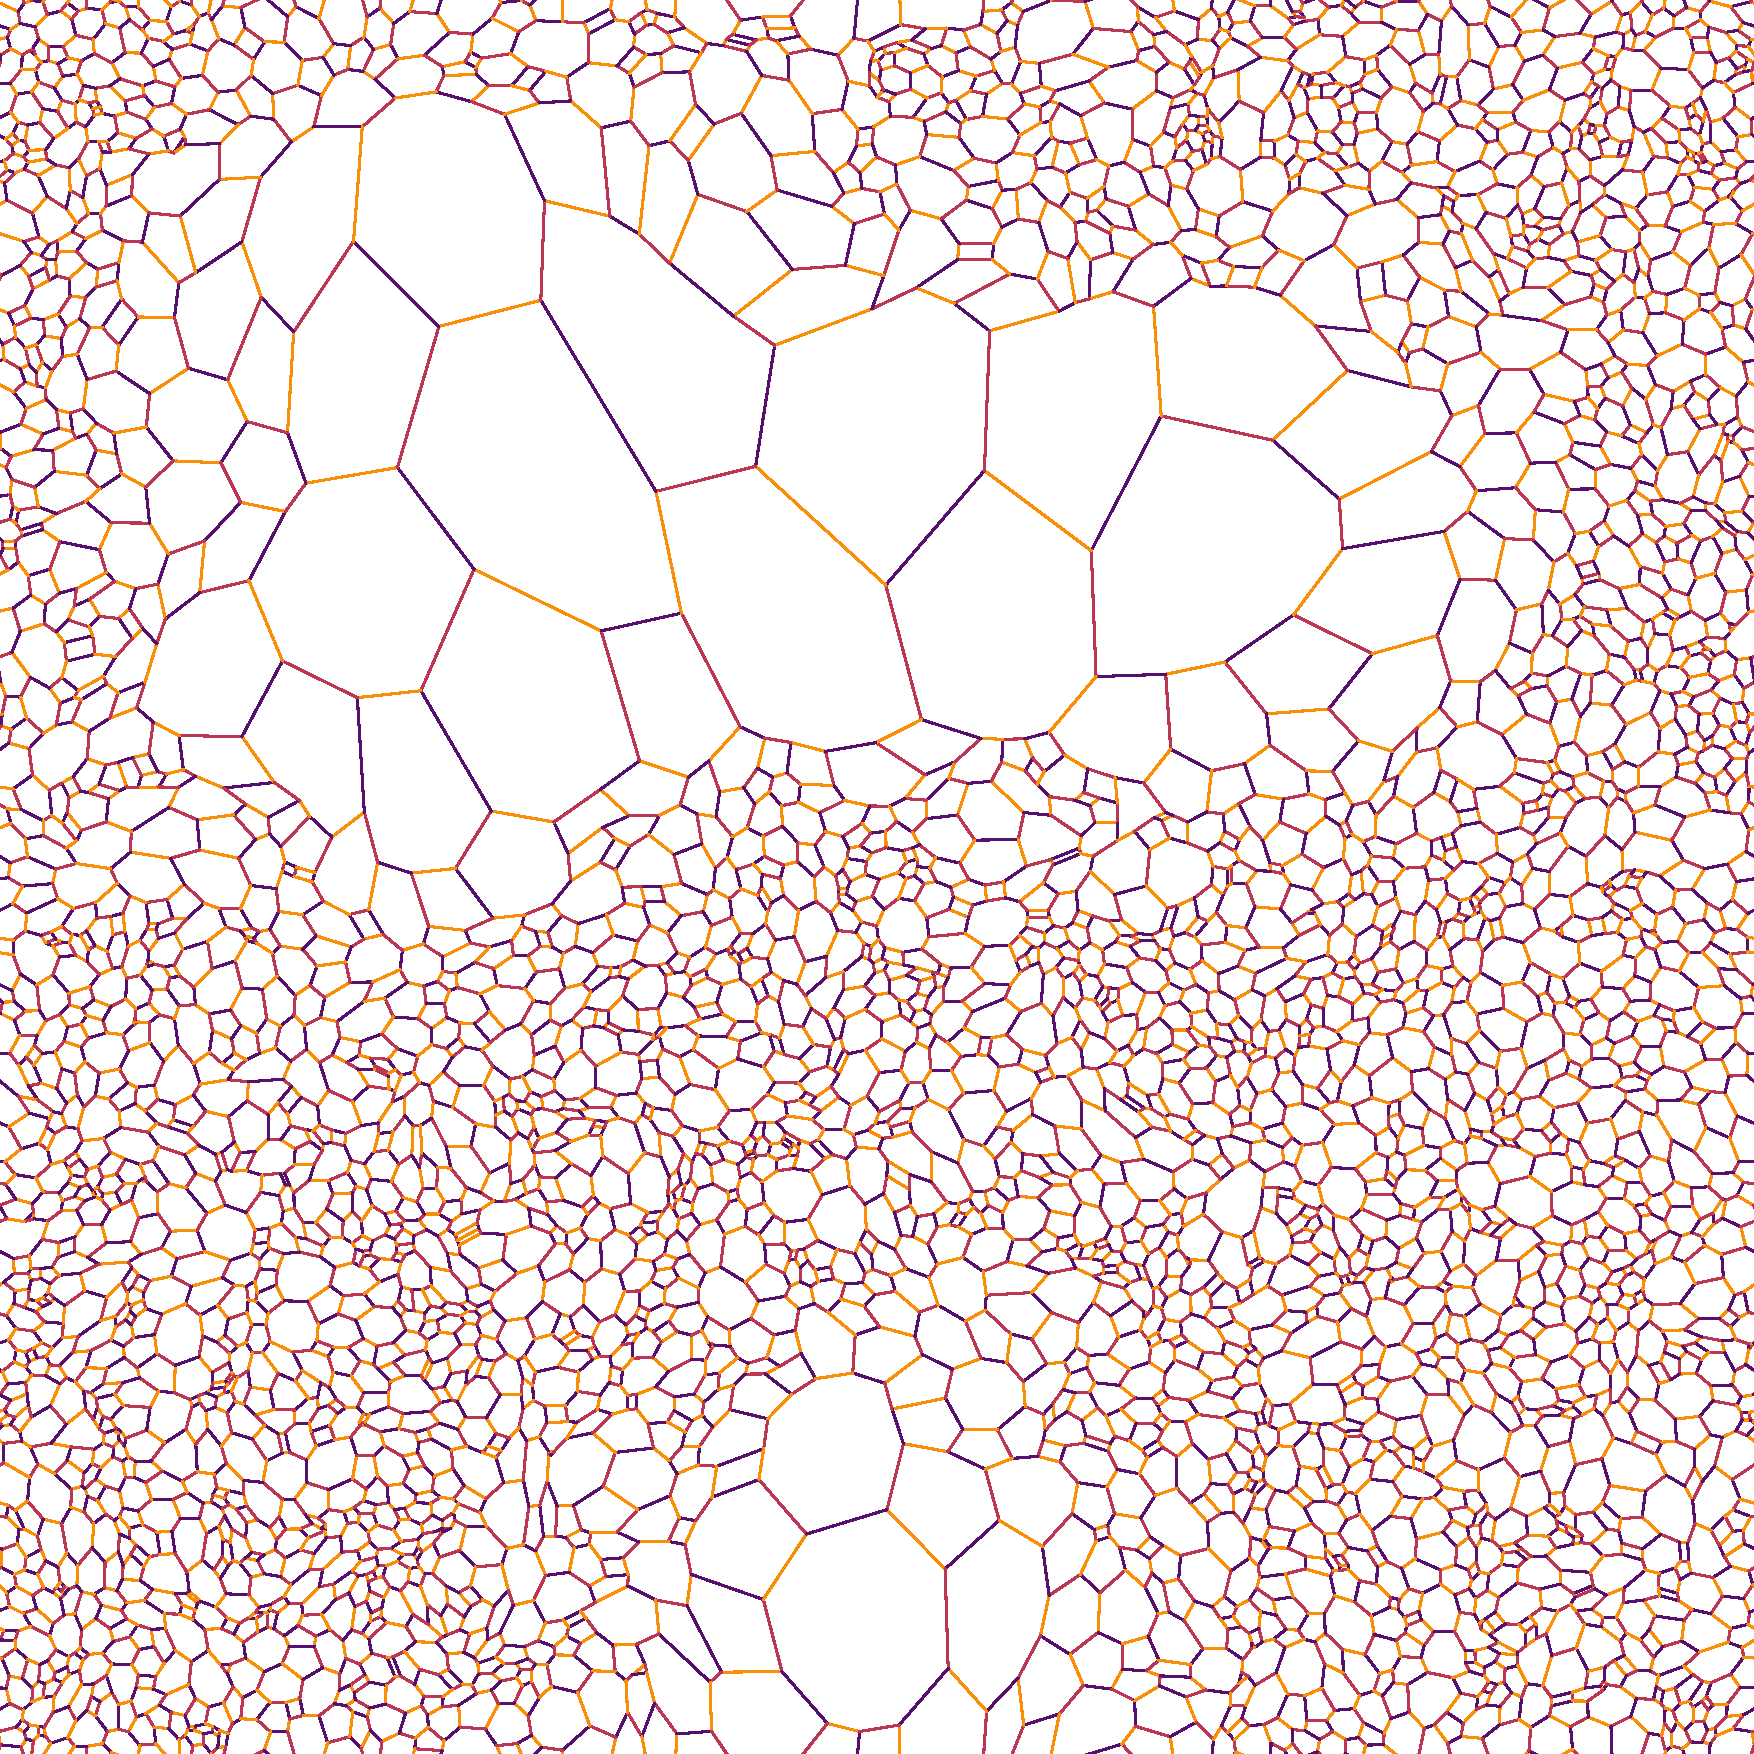
\includegraphics[width=297mm, height=297mm]{figure_code/amk_chapter_background_color.pdf}}}
\BgThispage
\begin{refsection}
\textbf{Contributions}

The material in this chapter expands on work presented in

~\autocite{cassellaExactChiralAmorphous2022} Cassella, G., D'Ornellas, P., Hodson, T., Natori, W. M., \& Knolle, J. (2022). An exact chiral amorphous spin liquid. \emph{arXiv preprint arXiv:2208.08246.}

All the code is available online~\autocite{hodsonKoalaKitaevAmorphous2022}.

This was a joint project of Gino, Peru and myself with advice and guidance from Willian and Johannes (all authors of the above). The project grew out of an interest the three of us had in studying amorphous systems, coupled with Johannes' expertise on the Kitaev model. The idea to use Voronoi partitions came from~\autocite{marsalTopologicalWeaireThorpe2020} and Gino did the implementation of this. The idea and implementation of the edge colouring using SAT solvers and the mapping from flux sector to bond sector using A* search were both entirely my work. Peru produced the numerical evidence for the ground state and implemented the local markers. Gino and I did much of the rest of the programming for Koala collaboratively, often pair programming, this included the phase diagram, edge mode and finite temperature analyses as well as the derivation of the projector in the amorphous case.

\hypertarget{amk-Model}{%
\section{The Model}\label{amk-Model}}

Already at its introduction it was known that Kitaev honeycomb model would remain solvable on any tri-coordinated graph. This has been used to generalise the model to many lattices~\autocite{eschmannThermodynamicClassificationThreedimensional2020,Yao2009,eschmann2019thermodynamics,Peri2020} but so far none have fully broken the translation symmetry of the model by putting it onto a amorphous lattice.

Amorphous lattices are characterised by local constraints but no long range order. These arise, for instance, in amorphous semiconductors~like Silicon and Germanium~\autocite{Yonezawa1983,zallen2008physics}. Recent work has shown that topological insulating (TI) phases, characterized by protected edge states and topological bulk invariants, can exist in amorphous systems~\autocite{mitchellAmorphousTopologicalInsulators2018,agarwala2019topological,marsalTopologicalWeaireThorpeModels2020,costa2019toward,agarwala2020higher,spring2021amorphous,corbae2019evidence}. TI phases, however, arise in non-interacting systems. In this context, we might ask whether QSL systems and the KH model in particular could be realised on amorphous lattices. The phases of the KH model have many similarities with TIs but differ in that the KH model is an interacting system. In general, research on amorphous electronic systems has been focused mainly on non-interacting systems with the exception of amorphous superconductivity~\autocite{buckel1954einfluss,mcmillan1981electron,meisel1981eliashberg,bergmann1976amorphous,mannaNoncrystallineTopologicalSuperconductors2022} or very recent work looking to understand the effect of strong electron repulsion in TIs~\autocite{kim2022fractionalization}.

Looking more towards the KH model, magnetism in amorphous systems has been investigated since the 1960s, mostly through the adaptation of theoretical tools developed for disordered systems~\autocite{aharony1975critical,Petrakovski1981,kaneyoshi1992introduction,Kaneyoshi2018}. We have already seen that the topological disorder of amorphous lattices can be qualitatively different from standard bond or site disorder, especially in two dimensions~\autocite{barghathiPhaseTransitionsRandom2014,schrauthViolationHarrisBarghathiVojtaCriterion2018}. Research focused on classical Heisenberg and Ising models has accounted for the observed behaviour of ferromagnetism, disordered antiferromagnetism and widely observed spin glass behaviour~\autocite{coey1978amorphous}. However, the role of the spin-anisotropic interactions and quantum effects that we see in the KH model has not been addressed in amorphous magnets. It is an open question whether frustrated magnetic interactions on amorphous lattices can give rise genuine quantum phases such as QSLs~\autocite{Anderson1973,Knolle2019,Savary2016,Lacroix2011}. This chapter will answer that question by demonstrating that the Kitaev model on amorphous lattices leads to a kind of QSL called a chiral spin liquid (CSL).

In this section I will discuss how to generalise the Kitaev model to an amorphous lattice. The methods section discusses how to generate such lattices using Voronoi partitions of the plane~\autocite{mitchellAmorphousTopologicalInsulators2018,marsalTopologicalWeaireThorpeModels2020}, colour them using a SAT solver and how to map back and forth between gauge field configurations and flux configurations. In the results section, I will show extensive numerical evidence that the model follows the simple generalisation to Lieb's theorem~\autocite{lieb_flux_1994} found by other works~\autocite{eschmannThermodynamicClassificationThreedimensional2020,Yao2009,eschmann2019thermodynamics,Peri2020}. I then map out the phase diagram of the model and show that the chiral phase around the symmetric point (\(J_x = J_y = J_z\)) is gapped and non-Abelian as characterized by a quantized local Chern number \(\nu\)~\autocite{peru_preprint,mitchellAmorphousTopologicalInsulators2018} as well as protected chiral Majorana edge modes. Finally, I look at the role of finite temperature fluctuations and show that the proliferation of flux excitations leads to an Anderson transition (similar to that of the FK model) to a thermal metal phase~\autocite{Laumann2012,lahtinenTopologicalLiquidNucleation2012,selfThermallyInducedMetallic2019}. Finally I consider possible physical realisations of the model and other generalisations.

\hypertarget{fig:amk-zoom}{%
\begin{figure}
\centering
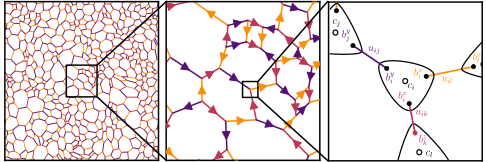
\includegraphics[width=1\textwidth,height=\textheight]{figure_code/amk_chapter/intro/amk_zoom/amk_zoom_by_hand}
\caption[{The Kitaev Honeycomb Model}]{\textbf{(a)} The standard Kitaev model is defined on a honeycomb lattice. The special feature of the honeycomb lattice that makes the model solvable is that each vertex is joined by exactly three bonds, i.e.~the lattice is trivalent. One of three labels is assigned to each \textbf{(b)}. We represent the antisymmetric gauge degree of freedom \(u_{jk} = \pm 1\) with arrows that point in the direction \(u_{jk} = +1\) \textbf{(c)}. The Majorana transformation can be visualised as breaking each spin into four Majoranas which then pair along the bonds. The pairs of x,y and z Majoranas become part of the classical \(\mathbb{Z}_2\) gauge field \(u_{ij}\). This leaves a single Majorana \(c_i\) per site.}
\label{fig:amk-zoom}
\end{figure}
}

The KH model must remain solvable on any lattice which satisfies two properties. First the lattice must first be trivalent, every vertex must three edges attached to it~\autocite{kitaevAnyonsExactlySolved2006,Nussinov2009}. A well studied class of amorphous trivalent lattices are the 2D Voronoi lattices~\autocite{mitchellAmorphousTopologicalInsulators2018,florescu_designer_2009,marsalTopologicalWeaireThorpeModels2020}. These arise from Voronoi partitions of the plane. Given a set of seed points, the Voronoi partition divides the plane into regions based on which seed point is closest by some metric, usually the euclidean metric. The `spheres of influence' of each seed point form the plaquettes of the resulting lattices, while the boundaries become the edges. The Voronoi partition exists in arbitrary dimensions and produces lattices with coordination number \(d+1\) except for degenerate cases with measure zero~\autocite{voronoiNouvellesApplicationsParamètres1908,watsonComputingNdimensionalDelaunay1981}. Hence Voronoi lattices in two dimensions lends themselves naturally to the Kitaev model.

Other methods of lattice generation are possible, one can connect randomly placed sites based on proximity~\autocite{agarwala2019topological} or create simplices from random sites~\autocite{christRandomLatticeField1982}. However these methods do not present a natural way to restrict the vertex degree to a constant. Perhaps ideally, we would sample uniformly from the space of possible trivalent graphs, there has been some work on how to do this using a Markov Chain Monte Carlo approach~\autocite{alyamiUniformSamplingDirected2016}. However, it does not guarantee that the resulting graph is planar, which is necessary to be able to 3-edge-colour the lattice, our second constraint.

The second constraint required for the Kitaev model to remain solvable is that we must be able to assign labels to each bond \(\{x,y,z\}\) such that each no two edges of the same label meet at a vertex. Such an assignment is is known as a 3-edge-colouring. For translation invariant models we need only find a solution for the unit cell which is usually small enough that this can be done by hand. For amorphous lattices the difficulty is compounded by the fact that, to the best of my knowledge, the problem of edge-colouring is in NP. To find colourings in practice, we will employ a standard method from the computer science literature for finding solutions of NP problems called a SAT solver, this is discussed in more detail in the \protect\hyperlink{amk-methods}{methods secton}.

We find that for larger lattices there are many valid colourings. In the isotropic case \(J^\alpha = 1\) the colouring has no physical significance. As the definition of the four Majoranas at a site is arbitrary, we can define a local operator that transforms the colouring of any particular site to another permutation and show that these operators commute with the Hamiltonian, see \protect\hyperlink{lattice-colouring}{appendix A.4}. We cannot do this in the anisotropic case but we nevertheless expect the lattices to exhibit a self averaging behaviour in larger systems when the colouring is chosen arbitrarily.

\hypertarget{fig:state_decomposition_animated}{%
\begin{figure}
\centering
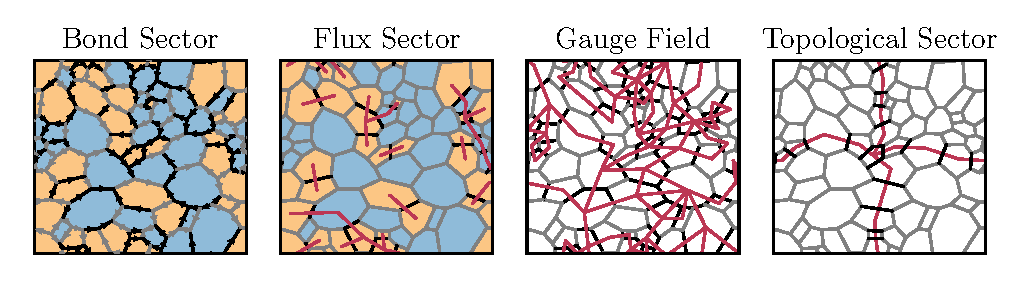
\includegraphics[width=1\textwidth,height=\textheight]{figure_code/amk_chapter/intro/state_decomposition_animated/state_decomposition_animated}
\caption[{State Decomposition}]{(Bond Sector) A state in the bond sector is specified by assigning \(\pm 1\) to each edge of the lattice. However, this description has a substantial gauge degeneracy. We can simplify things by decomposing each state into the product of three kinds of objects: (Vortex Sector) Only a small number of bonds need to be flipped (compared to some arbitrary reference) to reconstruct the vortex sector. Here, the edges are chosen from a spanning tree of the dual lattice, so there are no loops. (Gauge Field) The `loopiness' of the bond sector can be factored out. This gives a network of loops that can always be written as a product of the gauge operators \(D_j\). (Topological Sector) Finally, there are two loops that have no effect on the vortex sector, nor can they be constructed from gauge symmetries. These can be thought of as two fluxes \(\Phi_{x/y}\) that thread through the major and minor axes of the torus. Measuring \(\Phi_{x/y}\) amounts to constructing Wilson loops around the axes of the torus. We can flip the value of \(\Phi_{x}\) by transporting a vortex pair around the torus in the \(y\) direction, as shown here. In each of the three figures on the right, black bonds correspond to those that must be flipped. Composing the three together gives back the original bond sector on the left. \href{http://thomashodson.com/assets/thesis/amk_chapter/intro/state_decomposition_animated/state_decomposition_animated.gif}{ Animated version online.}}
\label{fig:state_decomposition_animated}
\end{figure}
}

On a lattice with the above properties, the solution laid out in~\protect\hyperlink{bg-hkm-model}{the kitaev model} remains applicable to our Amorphous Kitaev (AK) model. See \cref{fig:amk-zoom} for an example lattice generated by our method. The main differences are twofold. Firstly, the lattices are no longer bipartite in general and therefore contain plaquettes with an odd number of sides which have flux \(\pm i\). This leads the AK model to have a ground state with spontaneously broken chiral symmetry~\autocite{Chua2011,yaoExactChiralSpin2007,ChuaPRB2011,Fiete2012,Natori2016,Wu2009,Peri2020,WangHaoranPRB2021}. This is also similar to the behaviour of the original Kitaev model in response to a magnetic field. One ground state is related to the other by globally inverting the imaginary \(\phi_i\) fluxes~\autocite{yaoExactChiralSpin2007}.

Secondly, as the model is no longer translationally invariant, Lieb's theorem for the ground state flux sector no longer applies. However as discussed in the background, a simple generalisation of Lieb's theorem has been shown numerically to be applicable to many generalised Kitaev models~\autocite{eschmannThermodynamicClassificationThreedimensional2020,Yao2009,eschmann2019thermodynamics,Peri2020}. This generalisation states that the ground state flux configuration depends on on the number of sides of each plaquette \(\phi = -(\pm i)^{n_{\mathrm{sides}}}\) with a twofold global chiral degeneracy.

The obvious approach would be to verify that this generalises to the AK model numerically via exhaustive checking of flux configurations. However this is problematic because the number of states to check scales exponentially with system size. We side step this by gluing together two methods, we first work with lattices small enough that we can fully enumerate their flux sectors but tile them to reduce finite size effects. We then show that the effect of tiling scales away with system size.

\hypertarget{fig:majorana_bound_states}{%
\begin{figure}
\centering
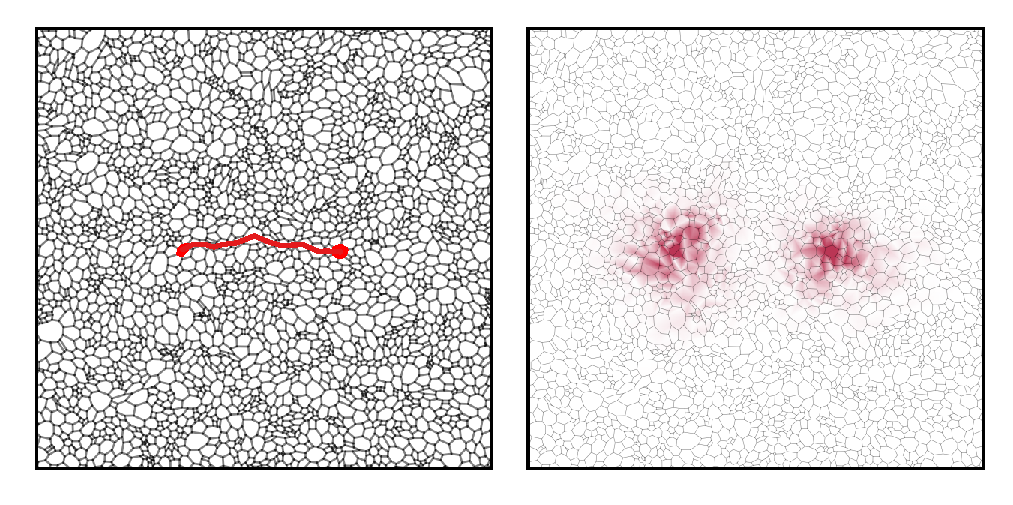
\includegraphics[width=1\textwidth,height=\textheight]{figure_code/amk_chapter/majorana_bound_states/majorana_bound_states}
\caption[{Majorana Bound States}]{(Left) A large amorphous lattice in the ground state save for a single pair of vortices shown in red, separated by the string of bonds that we flipped to create them. (Right) The density of the lowest energy Majorana state in this vortex sector. These Majorana states are bound to the vortices. They `dress' the vortices to create a composite object.}
\label{fig:majorana_bound_states}
\end{figure}
}

In order to evaluate the Chern marker later, we need a way to evaluate the model on open boundary conditions. Simply removing bonds from the lattice leaves behind unpaired \(b^\alpha\) operators that must be paired in some way to arrive at fermionic modes. To fix a pairing, we always start from a lattice defined on the torus and generate a lattice with open boundary conditions by defining the bond coupling \(J^{\alpha}_{ij} = 0\) for sites joined by bonds \((i,j)\) that we want to remove. This creates fermionic zero modes \(u_{ij}\) associated with these cut bonds which we set to 1 when calculating the projector. Alternatively, since all the fermionic zero modes are degenerate anyway, an arbitrary pairing of the unpaired \(b^\alpha\) operators could be performed.

\hypertarget{the-euler-equation}{%
\subsection{The Euler Equation}\label{the-euler-equation}}

Euler's equation provides a convenient way to understand how the states of the AK model factorise into flux sectors, gauge sectors and topological sectors. The Euler equation states if we embed a lattice with \(B\) bonds, \(P\) plaquettes and \(V\) vertices onto a closed surface of genus \(g\), (\(0\) for the sphere, \(1\) for the torus) then

\[B = P + V + 2 - 2g\]

For the case of the torus where \(g = 1\), we can rearrange this and exponentiate it to read:

\[2^B = 2^{P-1}\cdot 2^{V-1} \cdot 2^2\]

There are \(2^B\) configurations of the bond variables \(\{u_{ij}\}\). Each of these configurations can be uniquely decomposed into a flux sector, a gauge sector and a topological sector, see \cref{fig:state_decomposition_animated}. Each of the \(P\) plaquette operators \(\phi_i\) takes two values but vortices are created in pairs so there are \(2^{P-1}\) vortex sectors in total. There are \(2^{V-1}\) gauge symmetries formed from the \(V\) symmetry operators \(D_i\) because \(\prod_{j} D_j = \mathbb{I}\) is enforced by the projector. Finally, the two topological fluxes \(\Phi_x\) and \(\Phi_y\) account for the last factor of \(2^2\).

In addition, the fact that we only work with trivalent lattices implies that each vertex shares three bonds with other vertices so effectively comes with \(\tfrac{3}{2}\) bonds. This is consistent with the fact that, in the Majorana representation on the torus, each vertex brings three \(b^\alpha\) operators which then pair along bonds to give \(3/2\) bonds per vertex. Substituting \(3V = 2B\) into Euler's equation tells us that any trivalent lattice on the torus with \(N\) plaquettes has \(2N\) vertices and \(3N\) bonds. Since each bond is part of two plaquettes this implies that the mean number of sides of a plaquette is exactly six and that odd sides plaquettes must come in pairs.

\hypertarget{gauge-fields}{%
\subsection{Gauge Fields}\label{gauge-fields}}

The bond operators \(u_{ij}\) are useful because they label a bond sector \(\mathcal{\tilde{L}}_u\) in which we can easy solve the Hamiltonian. However, the gauge operators move us between bond sectors. \textbf{Bond sectors are not gauge invariant!}

Let us consider instead the properties of the plaquette operators \(\hat{\phi}_i\) that live on the faces of the lattice.

We already showed that they are conserved. As one might hope and expect, the plaquette operators also map cleanly onto the bond operators of the Majorana representation:

\[\begin{aligned}
\tilde{W}_p &= \prod_{\mathrm{i,j}\; \in\; p} \tilde{K}_{ij}\\
            &= \prod_{\mathrm{i,j}\; \in\; p} \tilde{\sigma}_i^\alpha \tilde{\sigma}_j^\alpha\\
            &= \prod_{\mathrm{i,j}\; \in\; p} (ib^\alpha_i c_i)(ib^\alpha_j c_j)\\
            &= \prod_{\mathrm{i,j}\; \in\; p} i u_{ij} c_i c_j\\
            &= \prod_{\mathrm{i,j}\; \in\; p} i u_{ij}
\end{aligned}\]

Where the last steps hold because each \(c_i\) appears exactly twice and is adjacent to its neighbour in each plaquette operator. This is consistent with the earlier observation that each \(W_p\) takes values \(\pm 1\) for even paths and \(\pm i\) for odd paths.

\hypertarget{vortices-and-their-movements}{%
\subsubsection{Vortices and their movements}\label{vortices-and-their-movements}}

\hypertarget{fig:types_of_dual_loops_animated}{%
\begin{figure}
\centering
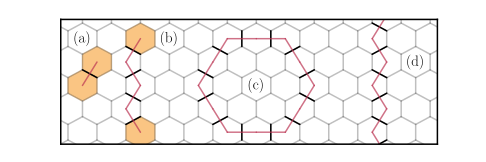
\includegraphics[width=1\textwidth,height=\textheight]{figure_code/amk_chapter/intro/types_of_dual_loops_animated/types_of_dual_loops_animated}
\caption[{Dual Loops and Vortex Pairs}]{\textbf{Dual Loops and Vortex Pairs} The different kinds of strings and loops that we can make by flipping bond variables or transporting vortices around. (a) Flipping a single bond makes a pair of vortices on either side. (b) Flipping a string of bonds separates the vortex pair spatially. The flipped bonds form a path (in red) on the dual lattice. (c) If we create a vortex-vortex pair, transport one of them around a loop and then annihilate them, we can change the bond sector without changing the vortex sector. This is a manifestation of the gauge symmetry of the bond sector. (d) If we transport a vortex around the major or minor axes of the torus, we create a non-contractable loop of bonds \(\hat{\mathcal{T}}_{x/y}\). Unlike all the other dual loops, These operators cannot be constructed from the contractable loops created by \(D_j\). operators and they flip the value of the topological fluxes. \href{http://thomashodson.com/assets/thesis/figure_code/amk_chapter/intro/types_of_dual_loops_animated/types_of_dual_loops_animated.gif}{ Animated version online.}}
\label{fig:types_of_dual_loops_animated}
\end{figure}
}

See \cref{fig:types_of_dual_loops_animated} for a diagram of the next three paragraphs.

We started from the ground state of the model and flipped the sign of a single bond (\cref{fig:types_of_dual_loops_animated} (a)). In doing so, we will flip the sign of the two plaquettes adjacent to that bond. We will call these disturbed plaquettes \emph{vortices}. We will refer to a particular choice values for the plaquette operators as a \emph{vortex sector}.

If we chain multiple bond flips, we can create a pair of vortices at arbitrary locations (\cref{fig:types_of_dual_loops_animated} (b)). The chain of bonds that we must flip corresponds to a path on the dual of the lattice.

We can also create a pair of vortices, move one around a loop and finally annihilate it with its partner (\cref{fig:types_of_dual_loops_animated} (c)). This corresponds to a closed loop on the dual lattice. Applying such a bond flip leaves the vortex sector unchanged. We can also do the same thing but move the vortex around one the non-contractible loops of the lattice (\cref{fig:types_of_dual_loops_animated} (d)).

\hypertarget{dual-loops-and-gauge-symmetries}{%
\subsubsection{Dual Loops and gauge symmetries}\label{dual-loops-and-gauge-symmetries}}

\hypertarget{fig:gauge_symmetries}{%
\begin{figure}
\centering
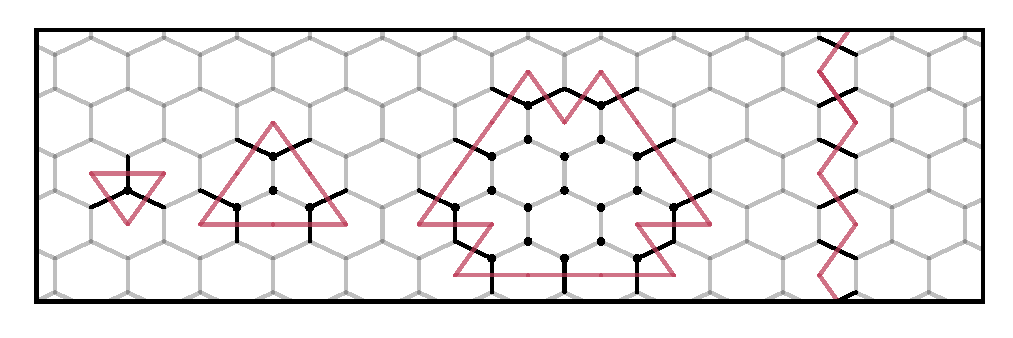
\includegraphics[width=1\textwidth,height=\textheight]{figure_code/amk_chapter/intro/gauge_symmetries/gauge_symmetries}
\caption[{Gauge Symmetries}]{\textbf{Dual Loops and Gauge Symmetries} A honeycomb lattice with edges in light grey, along with its dual, the triangle lattice in light blue. The vertices of the dual lattice are the faces of the original lattice and, hence, are the locations of the vortices. (Left) The action of the gauge operator \(D_j\) at a vertex is to flip the value of the three \(u_{jk}\) variables (black lines) surrounding site \(j\). The corresponding edges of the dual lattice (red lines) form a closed triangle. (Middle) Composing multiple adjacent \(D_j\) operators produces a large closed dual loop or multiple disconnected dual loops. Dual loops are not directed like Wilson loops. (Right) A non-contractable loop which cannot be produced by composing \(D_j\) operators. All three operators can be thought of as the action of a vortex-vortex pair that is created, one of them is transported around the loop, and then the two annihilate again. Note that every plaquette has an even number of \(u_{ij}\)s flipped on its edge. Therefore, all retain the same value.}
\label{fig:gauge_symmetries}
\end{figure}
}

See \cref{fig:gauge_symmetries} for a diagram of the next few paragraphs.

Notice that the \(D_j\) operators flip three bonds around a vertex. This is the smallest dual loop around which one can move a vortex pair and then annihilate it with itself.

Such operations compose, so we can build any larger loop (almost) by applying a series of \(D_j\) operations. The symmetrisation procedure \(\prod_i \left( \frac{1 + D_i}{2}\right)\) that maps from the bond sector to a physical state is really constructing a superposition over every such dual loops that leaves the vortex sector unchanged.

There is one kind of dual loop that we cannot build out of \(D_j\)s, the non-contractible loops.

\textbf{The plaquette operators and topological fluxes are the gauge invariant quantities which determine the physics of the model}

\hypertarget{composition-of-wilson-loops}{%
\subsubsection{Composition of Wilson loops}\label{composition-of-wilson-loops}}

\hypertarget{fig:plaquette_addition_by_hand}{%
\begin{figure}
\centering
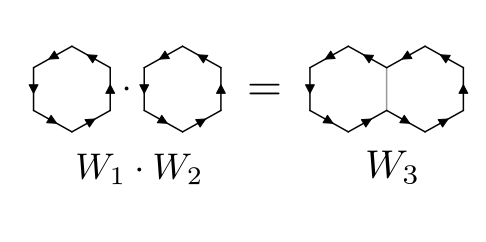
\includegraphics[width=0.57\textwidth,height=\textheight]{figure_code/amk_chapter/plaquette_addition/plaquette_addition_by_hand}
\caption[{Wilson Loop Composition}]{In the product of individual plaquette operators, shared bonds cancel out. The product is equal to the enclosing path.}
\label{fig:plaquette_addition_by_hand}
\end{figure}
}

Second, one can now easily show that the loops and plaquettes satisfy nice composition rules, so long as we keep to loops that wind in a particular direction.

Consider the product of two non-overlapping loops \(W_a\) and \(W_b\) that share an edge \(u_{12}\). Since the two loops both wind clockwise and do not overlap, one will contain a term \(i u_{12}\) and the other \(i u_{21}\). Since the \(u_{ij}\) commute with one another, they square to \(1\) and \(u_{ij} = -u_{ji}\), we have \(i u_{12} i u_{21} = 1\). We can repeat this for any number of shared edges. Hence, we get a version of Stokes' theorem: the product of \(i u_{jk}\) around any closed loop \(\partial A\) is equal to the product of plaquette operators \(\Phi\) that span the area \(A\) enclosed by that loop: \[\prod_{u_{jk} \in \partial A} i \; u_{jk} = \prod_{\phi_i \in A} \phi_i\]

\hypertarget{fig:stokes_theorem}{%
\begin{figure}
\centering
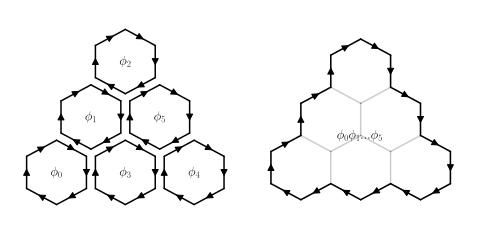
\includegraphics[width=0.71\textwidth,height=\textheight]{figure_code/amk_chapter/stokes_theorem/stokes_theorem}
\caption[{An analogue of Stokes' Theorem}]{The loop composition rule extends to arbitrary numbers of vortices which gives a discrete version of Stoke's theorem.}
\label{fig:stokes_theorem}
\end{figure}
}

Takeaway: Wilson loops can always be decomposed into products of plaquettes operators unless they are non-contractable.

\hypertarget{gauge-degeneracy-and-the-euler-equation}{%
\subsubsection{Gauge Degeneracy and the Euler Equation}\label{gauge-degeneracy-and-the-euler-equation}}

\hypertarget{fig:state_decomposition_animated}{%
\begin{figure}
\centering
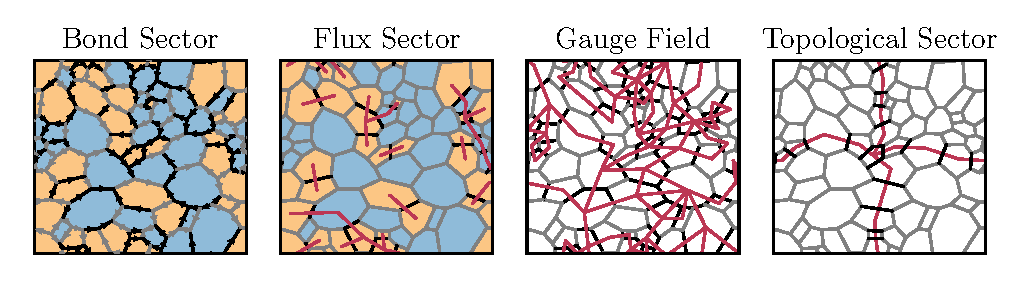
\includegraphics[width=1\textwidth,height=\textheight]{figure_code/amk_chapter/intro/state_decomposition_animated/state_decomposition_animated}
\caption[{State Decomposition}]{(Bond Sector) A state in the bond sector is specified by assigning \(\pm 1\) to each edge of the lattice. However, this description has a substantial gauge degeneracy. We can simplify things by decomposing each state into the product of three kinds of objects: (Vortex Sector) Only a small number of bonds need to be flipped (compared to some arbitrary reference) to reconstruct the vortex sector. Here, the edges are chosen from a spanning tree of the dual lattice, so there are no loops. (Gauge Field) The `loopiness' of the bond sector can be factored out. This gives a network of loops that can always be written as a product of the gauge operators \(D_j\). (Topological Sector) Finally, there are two loops that have no effect on the vortex sector, nor can they be constructed from gauge symmetries. These can be thought of as two fluxes \(\Phi_{x/y}\) that thread through the major and minor axes of the torus. Measuring \(\Phi_{x/y}\) amounts to constructing Wilson loops around the axes of the torus. We can flip the value of \(\Phi_{x}\) by transporting a vortex pair around the torus in the \(y\) direction, as shown here. In each of the three figures on the right, black bonds correspond to those that must be flipped. Composing the three together gives back the original bond sector on the left. \href{http://thomashodson.com/assets/thesis/figure_code/amk_chapter/intro/state_decomposition_animated/state_decomposition_animated.gif}{ Animated version online.}}
\label{fig:state_decomposition_animated}
\end{figure}
}

We can check this analysis with a counting argument. For a lattice with \(B\) bonds, \(P\) plaquettes and \(V\) vertices, we can count the number of bond sectors, vortices sectors and gauge symmetries and check them against Euler's polyhedra equation.

Euler's equation states for a closed surface of genus \(g\), i.e that has \(g\) holes so \(0\) for the sphere, \(1\) for the torus and \(g\) for \(g\) tori stuck together \[B = P + V + 2 - 2g\]

\hypertarget{fig:torus}{%
\begin{figure}
\centering
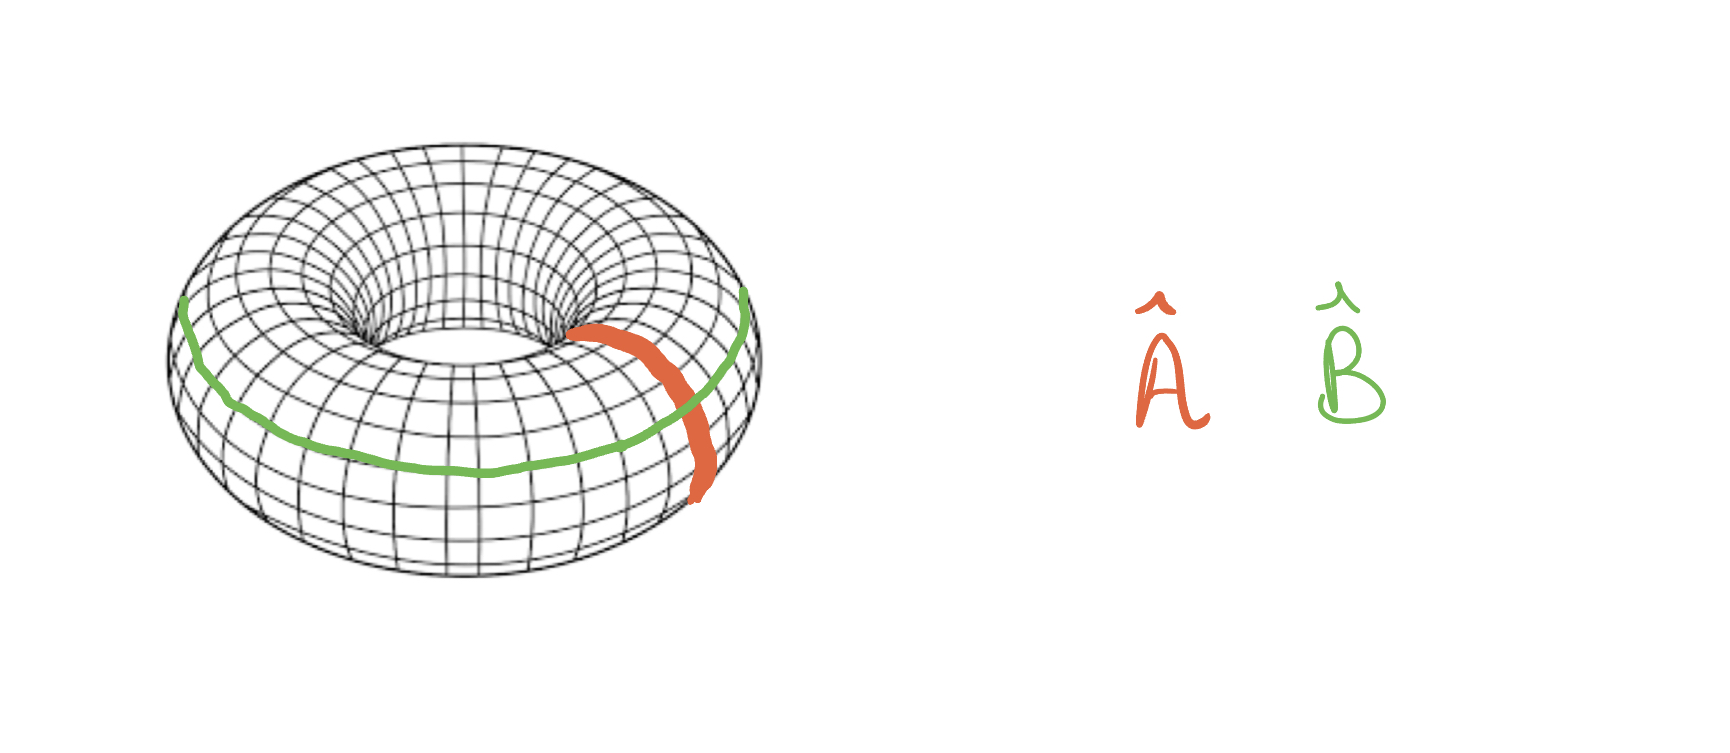
\includegraphics[width=0.86\textwidth,height=\textheight]{figure_code/amk_chapter/torus.jpeg}
\caption[{Loops on the Torus}]{In periodic boundary conditions the Kitaev model is defined on the surface of a torus. Topologically, the torus is distinct from the sphere in that it has a hole that cannot be smoothly deformed away. Associated with each such hole are two non-contractible loops on the surface, here labelled \(x\) and \(y\), which cannot be smoothly deformed to a point. These two non-contractible loops can be used to construct two special pairs of operators: The two topological fluxes \(\Phi_x\) and \(\Phi_y\) that are the expectation values of \(u_{jk}\) loops around each path. There are also two operators \(\hat{\mathcal{T}}_x\) and \(\hat{\mathcal{T}}_y\) that transform one half of a vortex pair around the loop before annihilating them together again, see later.}
\label{fig:torus}
\end{figure}
}

For the case of the torus where \(g = 1\), we can rearrange this to read: \[B = (P-1) + (V-1) + 2\]

\textbf{Bond Sectors}: Each \(u_{ij}\) takes two values and there is one associated with each bond so there are exactly \(2^B\) distinct configurations of the bond sector. Let us see if we can factor those configurations out into the Cartesian product of vortex sectors, gauge symmetries and non-contractible loop operators.

\textbf{Vortex sectors}: Each plaquette operator \(\phi_i\) takes two values (\(\pm 1\) or \(\pm i\)) and there are \(P\) of them. Vortices can only be created in pairs so there are \(\tfrac{2^P}{2} = 2^{P-1}\) vortex sectors in total. Denoting the number of pairs of vortices as \(N_v\), the vortex parity \(1 - 2*(N_v \mod 2)\) will be relevant in the projector later.

\textbf{Gauge symmetries}: As discussed earlier, these correspond to all possible compositions of the \(D_j\) operators. Again, there are only \(2^{V-1}\) of these because, as we will see in the next section, \(\prod_{j} D_j = \mathbb{1}\) in the physical space. We enforce this by choosing the correct product of single particle fermion states. One can get an intuitive picture for why \(\prod_{j} D_j = \mathbb{1}\) by imagining larger and larger patches of \(D_j\) operators on the torus. These patches correspond to transporting a vortex pair around the edge of the patch. At some point, the patch wraps around and starts to cover the entire torus. As this happens, the boundary of the patch disappears and, hence, it corresponds to the identity operation. See \cref{fig:flood_fill} and \cref{fig:flood_fill_amorphous}.

\textbf{Topological Sectors}: Finally, the torus has two non-contractible loop operators associated with its major and minor diameters. These give us two extra fluxes \(\Phi_x\) and \(\Phi_y\) each with two distinct values.

Putting this all together, we see that there are \textbf{\(2^B\) bond sectors} a space which can be decomposed into the Cartesian product of \textbf{\(2^{P-1}\) vortex sectors}, \textbf{\(2^{V-1}\) gauge symmetries} and \textbf{\(2^2 = 4\) topological sectors}.

The topological sector forms the basis of proposals to construct topologically protected qubits since the four sectors can only be mixed by a highly non-local perturbations \autocite{kitaevFaulttolerantQuantumComputation2003}.

Takeaway: The Extended Hilbert Space decomposes into a direct product of Flux Sectors, four Topological Sectors and a set of gauge symmetries.

\hypertarget{fig:flood_fill}{%
\begin{figure}
\centering
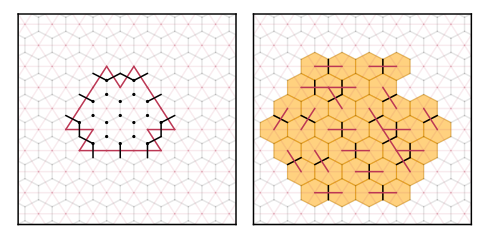
\includegraphics[width=1\textwidth,height=\textheight]{figure_code/amk_chapter/intro/flood_fill/flood_fill}
\caption[{Gauge Operators}]{A honeycomb lattice (in black) along with its dual (in red). (Left) Taking a larger and larger set of \(D_j\) operators (Bold Vertices) leads to an outward expanding boundary dual loop. Eventually every lattice on the torus is included and the boundary contracts to a point and disappears. This is a visual proof that \(\prod_i D_i \propto \mathbb{1}\). We'll see later that it takes values \(\pm 1\) and is a key part of the projection to the physical subspace. (Right) In black and red the edges and dual edges that must be flipped to add vortices at the sites highlighted in orange. Flipping all the \emph{plaquettes} in the system is \textbf{not} equivalent to the identity. Not that the edges that must be flipped can always be chosen from a tree since loops can be removed by a gauge transformation. \href{http://thomashodson.com/assets/thesis/figure_code/amk_chapter/intro/flood_fill/flood_fill.gif}{ Animated version online.}}
\label{fig:flood_fill}
\end{figure}
}

\hypertarget{counting-edges-plaquettes-and-vertices}{%
\subsubsection{Counting edges, plaquettes and vertices}\label{counting-edges-plaquettes-and-vertices}}

It is useful to know how the trivalent structure of the lattice constrains the number of bonds \(B\), plaquettes \(P\) and vertices \(V\) it has.

The lattice is built from vertices that each share three edges with their neighbours. This means that each vertex comes with \(\tfrac{3}{2}\) bonds i.e \(3V = 2B\). This is consistent with the fact that, in the Majorana representation on the torus, each vertex brings three \(b^\alpha\) operators which then pair along bonds to give \(3/2\) bonds per vertex.

If we define an integer \(N\) such that \(V = 2N\) and \(B = 3N\) and substitute this into the polyhedra equation for the torus, we see that \(P = N\). Therefore, if a trivalent lattice on the torus has \(N\) plaquettes, it has \(2N\) vertices and \(3N\) bonds.

We can also consider the sum of the number of bonds in each plaquette \(S_p\), since each bond is a member of exactly two plaquettes \[S_p = 2B = 6N\]

The mean size of a plaquette in a trivalent lattice on the torus is exactly six. As the sum is even, this also tells us that all odd plaquettes must come in pairs.

\hypertarget{fig:flood_fill_amorphous}{%
\begin{figure}
\centering
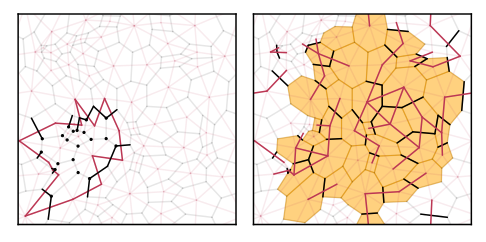
\includegraphics[width=1\textwidth,height=\textheight]{figure_code/amk_chapter/intro/flood_fill_amorphous/flood_fill_amorphous}
\caption[{Gauge Operators on Amorphous Lattices}]{The same as \cref{fig:flood_fill} but for the amorphous lattice. \href{http://thomashodson.com/assets/thesis/figure_code/amk_chapter/intro/flood_fill_amorphous/flood_fill_amorphous.gif}{ Animated version online.}}
\label{fig:flood_fill_amorphous}
\end{figure}
}

\hypertarget{the-projector}{%
\subsection{The Projector}\label{the-projector}}

The projection from the extended space to the physical space will not be particularly important for the results presented here. However, the theory remains useful to explain why this is.

\hypertarget{fig:hilbert_spaces}{%
\begin{figure}
\centering
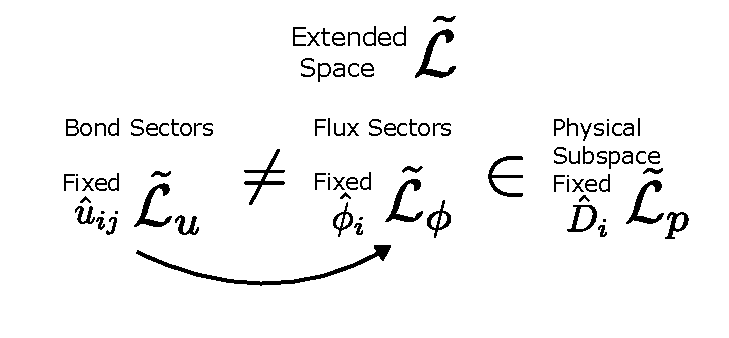
\includegraphics[width=1\textwidth,height=\textheight]{figure_code/amk_chapter/hilbert_spaces}
\caption[{How the different Hilbert Spaces relate to one another}]{The relationship between the different Hilbert spaces used in the solution. \textbf{needs updating}}
\label{fig:hilbert_spaces}
\end{figure}
}

The physical states are defined as those for which \(D_i |\phi\rangle = |\phi\rangle\) for all \(D_i\). Since \(D_i\) has eigenvalues \(\pm1\), the quantity \(\tfrac{(1+D_i)}{2}\) has eigenvalue \(1\) for physical states and \(0\) for extended states so is the local projector onto the physical subspace.

Therefore, the global projector is \[ \mathcal{P} = \prod_{i=1}^{2N} \left( \frac{1 + D_i}{2}\right)\]

for a toroidal trivalent lattice with \(N\) plaquettes \(2N\) vertices and \(3N\) edges. As discussed earlier, the product over \((1 + D_j)\) can also be thought of as the sum of all possible subsets \(\{i\}\) of the \(D_j\) operators, which is the set of all possible gauge symmetry operations.

\[ \mathcal{P} = \frac{1}{2^{2N}} \sum_{\{i\}} \prod_{i\in\{i\}} D_i\]

Since the gauge operators \(D_j\) commute and square to one, we can define the complement operator \(C = \prod_{i=1}^{2N} D_i\) and see that it takes each set of \(\prod_{i \in \{i\}} D_j\) operators and gives us the complement of that set. We will shortly see why \(C\) is the identity in the physical subspace, as noted earlier.

We use the complement operator to rewrite the projector as a sum over half the subsets of \(\{i\}\) - referred to as \(\Lambda\). The complement operator deals with the other half

\[ \mathcal{P} =  \left( \frac{1}{2^{2N-1}} \sum_{\Lambda} \prod_{i\in\{i\}} D_i\right) \left(\frac{1 + \prod_i^{2N} D_i}{2}\right) = \mathcal{S} \cdot \mathcal{P}_0\]

To compute \(\mathcal{P}_0\), the main quantity needed is the product of the local projectors \(D_i\) \[\prod_i^{2N} D_i = \prod_i^{2N} b^x_i b^y_i b^z_i c_i \] for a toroidal trivalent lattice with \(N\) plaquettes \(2N\) vertices and \(3N\) edges.

First, we reorder the operators by bond type. This does not require any information about the underlying lattice.

\[\prod_i^{2N} D_i = \prod_i^{2N} b^x_i \prod_i^{2N} b^y_i \prod_i^{2N} b^z_i \prod_i^{2N} c_i\]

The product over \(c_i\) operators reduces to a determinant of the Q matrix and the fermion parity, see \autocite{pedrocchiPhysicalSolutionsKitaev2011}. The only difference from the honeycomb case is that we cannot explicitly compute the factors \(p_x,p_y,p_z = \pm\;1\) that arise from reordering the b operators such that pairs of vertices linked by the corresponding bonds are adjacent.

\[\prod_i^{2N} b^\alpha_i = p_\alpha \prod_{(i,j)}b^\alpha_i b^\alpha_j\]

However, they are simply the parity of the permutation from one ordering to the other and can be computed in linear time with a cycle decomposition \textbf{cite}.

We find that \[\mathcal{P}_0 = 1 + p_x\;p_y\;p_z\; \hat{\pi} \; \mathrm{det}(Q^u) \; \prod_{\{i,j\}} -iu_{ij}\]

where \(p_x\;p_y\;p_z = \pm 1\) are lattice structure factors and \(\mathrm{det}(Q^u)\) is the determinant of the matrix mentioned earlier that maps \(c_i\) operators to normal mode operators \(b'_i, b''_i\). These depend only on the lattice structure.

\(\hat{\pi} = \prod{i}^{N} (1 - 2\hat{n}_i)\) is the parity of the particular many body state determined by fermionic occupation numbers \(n_i\). As discussed in \autocite{pedrocchiPhysicalSolutionsKitaev2011}, \(\hat{\pi}\) is gauge invariant in the sense that \([\hat{\pi}, D_i] = 0\).

This implies that \(det(Q^u) \prod -i u_{ij}\) is also a gauge invariant quantity. In translation invariant models this quantity which can be related to the parity of the number of vortex pairs in the system \autocite{yaoAlgebraicSpinLiquid2009}.

All these factors take values \(\pm 1\) so \(\mathcal{P}_0\) is 0 or 1 for a particular state. Since \(\mathcal{S}\) corresponds to symmetrising over all the gauge configurations and cannot be 0, once we have determined the single particle eigenstates of a bond sector, the true many body ground state has the same energy as either the empty state with \(n_i = 0\) or a state with a single fermion in the lowest level.

\hypertarget{ground-state-degeneracy}{%
\subsubsection{Ground State Degeneracy}\label{ground-state-degeneracy}}

\hypertarget{fig:loops_and_dual_loops}{%
\begin{figure}
\centering
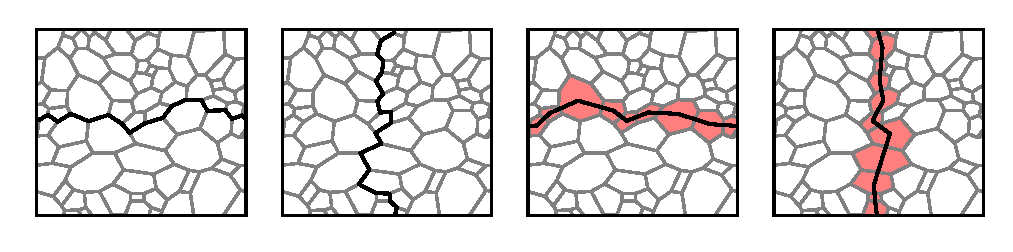
\includegraphics[width=1\textwidth,height=\textheight]{figure_code/amk_chapter/loops_and_dual_loops/loops_and_dual_loops}
\caption[{Topological Loops and Dual Loops}]{(Left) The two topological flux operators of the toroidal lattice. These do not correspond to any face of the lattice, but rather measure flux that threads through the major and minor axes of the torus. This shows a particular choice. Yet, any loop that crosses the boundary is gauge equivalent to one of or the sum of these two loop. (Right) The two ways to transport vortices around the diameters. These amount to creating a vortex pair, transporting one of them around the major or minor diameters of the torus and, then, annihilating them again.}
\label{fig:loops_and_dual_loops}
\end{figure}
}

More general arguments \autocite{chungExplicitMonodromyMoore2007,oshikawaTopologicalDegeneracyNonAbelian2007} imply that \(det(Q^u) \prod -i u_{ij}\) has an interesting relationship to the topological fluxes. In the non-Abelian phase, we expect that it will change sign in exactly one of the four topological sectors.

This means that the lowest state in three of the topological sectors contain no fermions, while in one of them there must be one fermion to preserve product of fermion vortex parity. So overall the non-Abelian model has a three-fold degenerate ground state rather than the fourfold of the Abelian case (and of my intuition!). In the Abelian phase, this does not happen and we get a fourfold degenerate ground state. \textbf{Whether this analysis generalises to the amorphous case is unclear.}

An alternative way to view this is to imagine we start in one state of the ground state manifold. We then attempt to construct other ground states by creating vortex pairs, transporting one vortex around one or both non-contractible loops and then annihilating them. This works for either of the two non-contractible loops but when we try to do it for \emph{both} something strange happens. When we transport a vortex around \textbf{both} the major and minor axes of the torus this changes its fusion channel. Normally two vortices fuse to the vacuum but after this operation they fuse into a fermion excitation. And hence our attempt to construct that last ground state doesn't yield a ground state at all, leaving us with just three.

\textbf{NOTE to self: This argument seems to involve adiabatic insertion of the fluxes \(\Phi_{x,y}\) as the operations that undo vortex transport around the lattice. I don't understand why that part is necessary}

\hypertarget{fig:threefold_degeneracy}{%
\begin{figure}
\centering
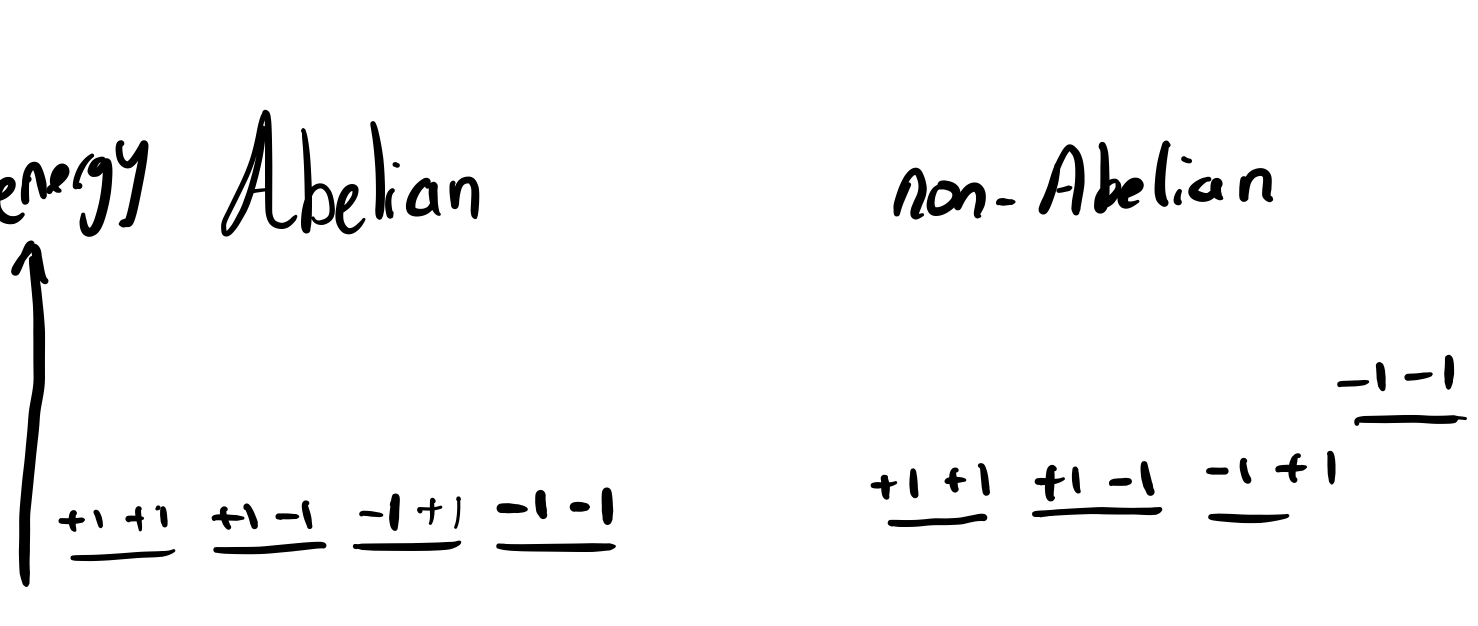
\includegraphics[width=0.86\textwidth,height=\textheight]{figure_code/amk_chapter/threefold_degeneracy.png}
\caption[{Ground State Degeneracy in the Abelian and Non-Abelian Phases}]{In the non-Abelian phase one of the lowest energy state in one of the topological sectors contains a fermion and hence is slightly higher in energy than the other three. This manifests as a fourfold ground state degeneracy in the Abelian phase and a threefold degeneracy in the non-Abelian phase.}
\label{fig:threefold_degeneracy}
\end{figure}
}

\hypertarget{quick-breather}{%
\subsubsection{Quick Breather}\label{quick-breather}}

Let's consider where are with the model now. We can map the spin Hamiltonian to a Majorana Hamiltonian in an extended Hilbert space. Along with that mapping comes a gauge field \(u_{jk}\) defining \textbf{bond sectors}. The gauge symmetries of \(u_{jk}\) are generated by the set of \(D_j\) operators. The gauge invariant, and, therefore, physically, relevant variables are the plaquette operators \(\phi_i\) which define as a \textbf{vortex sector}. To solve the Majorana Hamiltonian, we must remove hats from the gauge field by restricting ourselves to a particular bond sector. At this stage, the Majorana Hamiltonian becomes non-interacting and we can solve it like any quadratic theory. This lets us construct the single particle eigenstates from which we can also construct many body states. Yet, the many body states constructed in this way are not in the physical subspace!

For the many body states within a particular bond sector, \(\mathcal{P}_0 = 0,1\) tells us which of those overlap with the physical sector.

We see that finding a state that has overlap with a physical state only ever requires the addition or removal of one fermion. There are cases where this can make a difference, but for most observables, such as ground state energy, this correction scales away as the number of fermions in the system grows.

If we wanted to construct a full many body wavefunction in the spin basis, we would need to include the full symmetrisation over the gauge fields. However, this was not necessary for any of the results that will be presented here.

\hypertarget{the-ground-state}{%
\subsection{The Ground State}\label{the-ground-state}}

We have shown that the Hamiltonian is gauge invariant. As a result, only the flux sector and the two topological fluxes affect the spectrum of the Hamiltonian. Thus, we can label the many body ground state by a combination of fluxes and fermionic occupation numbers.

By studying the projector, we saw that the fermionic occupation numbers of the ground state will always be either \(n_m = 0\) or \(n_0 = 1, n_{m>1} = 0\) because the projector only enforces combined vortex and fermion parity.

I refer to the flux sector that contains the ground state as the ground state flux sector. Recall that the excitations of the fluxes away from the ground ground state configuration are called \textbf{vortices}, so that the ground state flux sector is, by definition, the vortex free sector.

On the Honeycomb, Lieb's theorem implies that the ground state corresponds to the state where all \(u_{jk} = 1\). This implies that the flux free sector is the ground state sector \autocite{lieb_flux_1994}.

Lieb's theorem does not generalise easily to the amorphous case. However, we can get some intuition by examining the problem that will lead to a guess for the ground state. We will then provide numerical evidence that this guess is in fact correct.

Consider the partition function of the Majorana hamiltonian: \[ \mathcal{Z} = \mathrm{Tr}\left( e^{-\beta H}\right) = \sum_i \exp{-\beta \epsilon_i}\] At low temperatures \(\mathcal{Z} \approx \beta \epsilon_0\) where \(\epsilon_0\) is the lowest energy fermionic state.

How does the \(\mathcal{Z}\) depend on the Majorana hamiltonian? Expanding the exponential out gives \[ \mathcal{Z} = \sum_n \frac{(-\beta)^n}{n!} \mathrm{Tr(H^k)} \]

This makes for an interesting observation. The Hamiltonian is essentially a scaled adjacency matrix. An adjacency matrix being a matrix \(g_{ij}\) such that \(g_{ij} = 1\) if vertices \(i\) and \(j\) and joined by an edge and 0 otherwise.

Powers of adjacency matrices have the property that the entry \((g^n)_{ij}\) corresponds to the number of paths of length \(n\) on the graph that begin at site \(i\) and end at site \(j\). These include somewhat degenerate paths that go back on themselves.

Therefore, the trace of an adjacency matrix \[\mathrm{Tr}(g^n) = \sum_i (g^n)_{ii}\] counts the number of loops of size \(n\) that can be drawn on the graph.

Applying the same treatment to our Majorana Hamiltonian, we can interpret \(u_{ij}\) to equal 0 if the two sites are not joined by a bond and we put ourselves in the isotropic phase where \(J^\alpha = 1\) \[ \tilde{H}_{ij} =  \tfrac{1}{2} i u_{ij}\]

We then see that the trace of the nth power of H is a sum over Wilson loops of size \(n\) with an additional factor of \(2^{-n}\). We showed earlier that the Wilson loop operators can always be written as products of the plaquette operators that they enclose.

Lumping all the prefactors together, we will get something schematically like: \[ \mathcal{Z} = c_A \hat{A} + c_B \hat{B} + \sum_i c_i \hat{\phi}_i + \sum_{ij} c_{ij}  \hat{\phi}_i \hat{\phi}_j + \sum_{ijk} c_{ijk}  \hat{\phi}_i \hat{\phi}_j \hat{\phi}_k + ...\]

Where the \(c\) factors would be something like \[c_{ijk...} = \sum_n \tfrac{(-\beta)^n}{n!} \tfrac{1}{2^n} K_{ijk...}\] This is a sum over all loop lengths \(n\) with, for each, a combinatorial factor \(K_{ijk...}\) that counts how many ways exist to draw a loop of length \(n\) that only encloses plaquettes \(ijk...\).

We also have the pesky topological fluxes \(\Phi_x\) and \(\Phi_y\). Again, the prefactors for these are very complicated. However, we can intuitively see that for larger and larger loops lengths, there will be a combinatorial explosion of possible ways that they appear in these sums. We know that explosion will be suppressed exponentially for sufficiently large system sizes but for practical lattices they cause significant finite size effects.

We do not have much hope of actually evaluating this for an amorphous lattice. However, we can guess that the ground state vortex sector might be a simple function of the side length of each plaquette.

The ground state of the Amorphous Kitaev Model is found by setting the flux through each plaquette \(\phi\) to be equal to \(\phi^{\mathrm{g.s.}}(n_{\mathrm{sides}})\)

\[\begin{aligned}
    \phi^{\mathrm{g.s.}}(n_{\mathrm{sides}}) = -(\pm i)^{n_{\mathrm{sides}}},
\end{aligned}\] where \(n_{\mathrm{sides}}\) is the number of edges that form each plaquette and the choice of sign gives a twofold chiral ground state degeneracy.

This conjecture is consistent with Lieb's theorem on regular lattices \autocite{lieb_flux_1994} and is supported by numerical evidence. As noted before, any flux that differs from the ground state is an excitation which we call a vortex.

\hypertarget{finite-size-effects}{%
\subsubsection{Finite size effects}\label{finite-size-effects}}

This guess only works for larger lattices. To rigorously test it, we would want to directly enumerate the \(2^N\) vortex sectors for a smaller lattice and check that the lowest state found is the vortex sector predicted by our conjecture.

To do this we tile an amorphous lattice as the unit cell of a periodic \(N\times N\) system. Bonds that originally crossed the periodic boundaries now connect adjacent unit cells. Using Bloch's theorem, the problem essentially reduces back to the single amorphous unit cell. However, now the edges that cross the periodic boundaries pick up a phase dependent on the crystal momentum \(\vec{q} = (q_x, q_y)\) and the lattice vector of the bond \(\vec{x} = (+1, 0, -1, +1, 0, -1)\). Assigning these lattice vectors to each bond is also a very convenient way to store and plot toroidal graphs.

This can then be solved using Bloch's theorem. For a given crystal momentum \(\textbf{q} \in [0,2\pi)^2\), we are left with a Bloch Hamiltonian, which is identical to the original Hamiltonian aside from an extra phase on edges that cross the periodic boundaries in the \(x\) and \(y\) directions, \[\begin{aligned}
    M_{jk}(\textbf{q}) =  \frac{i}{2} J^{\alpha} u_{jk} e^{i q_{jk}},\end{aligned}\] where \(q_{jk} = q_x\) for a bond that crosses the \(x\)-periodic boundary in the positive direction, with the analogous definition for \(y\)-crossing bonds. We also have \(q_{jk} = -q_{kj}\). Finally, \(q_{jk} = 0\) if the edge does not cross any boundaries at all. In essence, we are imposing twisted boundary conditions on our system. The total energy of the tiled system can be calculated by summing the energy of \(M( \textbf{q})\) for every value of \(\textbf{q}\).

With this technique, the finite size effects related to the non-contractible loop operators are removed with only a linear penalty in computation time compared to the exponential penalty paid by simply diagonalising larger lattices.

This technique verifies that \(\phi_0\) correctly predicts the ground state for hundreds of thousands of lattices with up to twenty plaquettes. For larger lattices, we verified that random perturbations around the predicted ground state never yield a lower energy state.

\hypertarget{chiral-symmetry}{%
\subsubsection{Chiral Symmetry}\label{chiral-symmetry}}

The discussion above shows that the ground state has a twofold \textbf{chiral} degeneracy which arises because the global sign of the odd plaquettes does not matter.

This happens because we have broken the time reversal symmetry of the original model by adding odd plaquettes \autocite{Chua2011,yaoExactChiralSpin2007,ChuaPRB2011,Fiete2012,Natori2016,Wu2009,Peri2020,WangHaoranPRB2021}.

Similarly to the behaviour of the original Kitaev model in response to a magnetic field, we get two degenerate ground states of different handedness. Practically speaking, one ground state is related to the other by inverting the imaginary \(\phi\) fluxes \autocite{yaoExactChiralSpin2007}.

\hypertarget{phases-of-the-kitaev-model}{%
\subsection{Phases of the Kitaev Model}\label{phases-of-the-kitaev-model}}

discuss the Abelian A phase / toric code phase / anisotropic phase

the isotropic gapless phase of the standard model

The isotropic gapped phase with the addition of a magnetic field

\hypertarget{what-is-so-great-about-two-dimensions}{%
\subsection{What is so great about two dimensions?}\label{what-is-so-great-about-two-dimensions}}

\hypertarget{topology-chirality-and-edge-modes}{%
\subsubsection{Topology, chirality and edge modes}\label{topology-chirality-and-edge-modes}}

Most thermodynamic and quantum phases studied can be characterised by a local order parameter. That is, a function or operator that only requires knowledge about some fixed sized patch of the system that does not scale with system size.

However, there are quantum phases that cannot be characterised by such a local order parameter. These phases are instead said to possess `topological order'.

One easily observable property of topological order is that the ground state degeneracy depends on the topology of the manifold that we put the system on to. This is referred to as topological degeneracy to distinguish it from standard symmetry breaking.

The Kitaev model is a good example. We have already looked at it defined on a graph that is embedded either into the plane or onto the torus. The extension to surfaces like the torus but with more than one handle is relatively easy.

\hypertarget{anyonic-statistics}{%
\subsubsection{Anyonic Statistics}\label{anyonic-statistics}}

\textbf{NB: I'm thinking about moving this section to the overall intro, but it's nice to be able to refer to specifics of the Kitaev model also so I'm not sure. It currently repeats a discussion of the ground state degeneracy from the projector section.}

In dimensions greater than two, the quantum state of a system must pick up a factor of \(-1\) or \(+1\) if two identical particles are swapped. We call these Fermions and Bosons.

This argument is predicated on the idea that performing two swaps is equivalent to doing nothing. Doing nothing should not change the quantum state at all. Therefore, doing one swap can at most multiply it by \(\pm 1\).

However, there are many hidden parts to this argument. First, this argument does not present the whole story. For instance, if you want to know why Fermions have half integer spin, you have to go to field theory.

Second, why does this argument only work in dimensions greater than two? When we say that two swaps do nothing, we in fact say that the world lines of two particles that have been swapped twice can be untangled without crossing. Why can't they cross? Because if they cross, the particles can interact and the quantum state could change in an arbitrary way. We are implicitly using the locality of physics to argue that, if the worldlines stay well separated, the overall quantum state cannot change.

In two dimensions, we cannot untangle the worldlines of two particles that have swapped places. They are braided together (see \cref{fig:braiding}).

\hypertarget{fig:braiding}{%
\begin{figure}
\centering
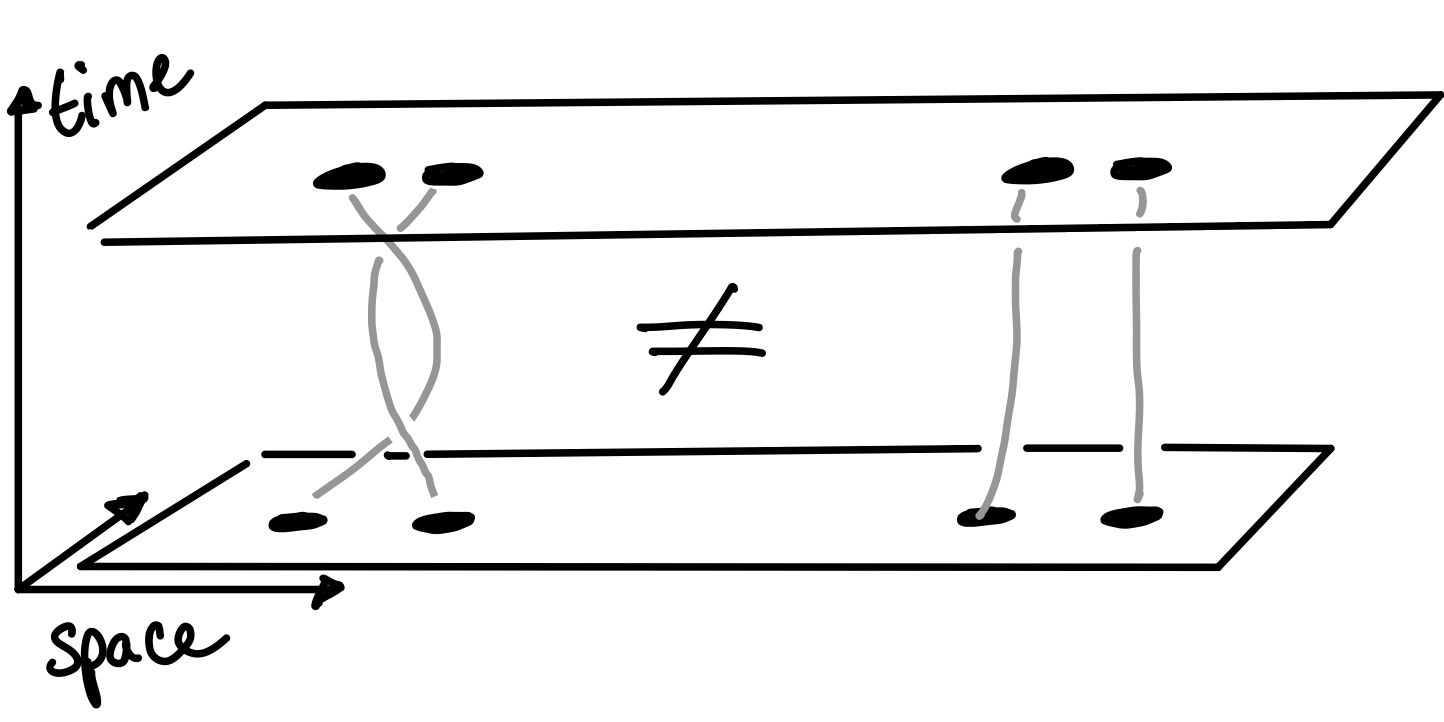
\includegraphics[width=0.71\textwidth,height=\textheight]{figure_code/amk_chapter/braiding.png}
\caption[{Braiding in Two Dimensions}]{Worldlines of particles in two dimensions can become tangled or \emph{braided} with one another.}
\label{fig:braiding}
\end{figure}
}

From this fact flows a whole of behaviours. The quantum state can acquire a phase factor \(e^{i\phi}\) upon exchange of two identical particles, which we now call Anyons.

The Kitaev Model is a good demonstration of the connection between Anyons and topological degeneracy. In the Kitaev model, we can create a pair of vortices, move one around a non-contractable loop \(\mathcal{T}_{x/y}\) and then annihilate them together. Without topology, this should leave the quantum state unchanged. Instead, we move towards another ground state in a topologically degenerate ground state subspace. Practically speaking, it flips a dual line of bonds \(u_{jk}\) going around the loop which we cannot undo with any gauge transformation made from \(D_j\) operators.

If the ground state subspace is multidimensional, quasiparticle exchange can move us around in the space with an action corresponding to a matrix. In general, these matrices do not commute so these are known as non-Abelian anyons.

From here, the situation becomes even more complex. The Kitaev model has a non-Abelian phase when exposed to a magnetic field. The amorphous Kitaev Model has a non-Abelian phase because of its broken chiral symmetry.

By subdividing the Kitaev model into vortex sectors, we neatly separate between vortices and fermionic excitations. However, if we looked at the full many body picture, we would see that a vortex carries with it a cloud of bound Majorana states.

\hypertarget{fig:majorana_bound_states}{%
\begin{figure}
\centering
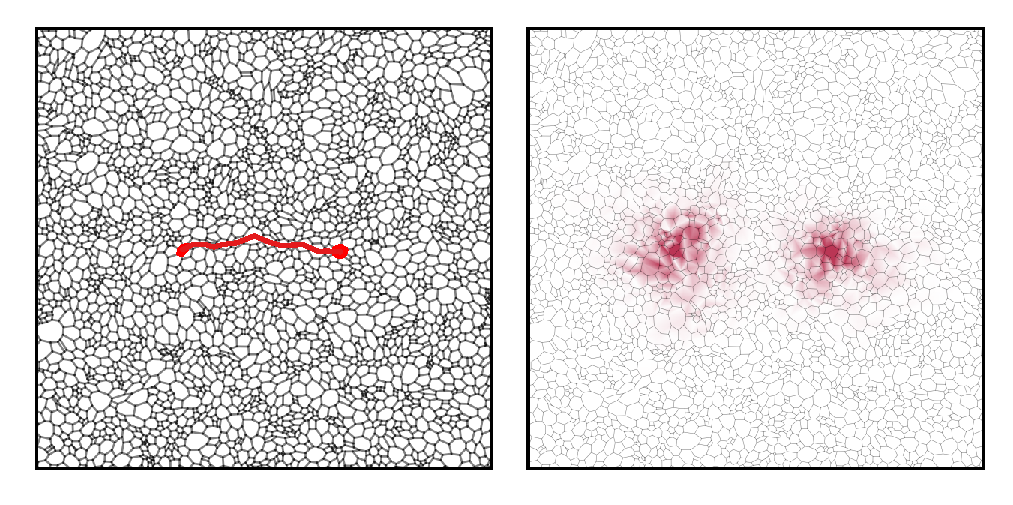
\includegraphics[width=1\textwidth,height=\textheight]{figure_code/amk_chapter/majorana_bound_states/majorana_bound_states}
\caption[{Majorana Bound States}]{(Left) A large amorphous lattice in the ground state save for a single pair of vortices shown in red, separated by the string of bonds that we flipped to create them. (Right) The density of the lowest energy Majorana state in this vortex sector. These Majorana states are bound to the vortices. They `dress' the vortices to create a composite object.}
\label{fig:majorana_bound_states}
\end{figure}
}

Consider two processes

\begin{enumerate}
\def\labelenumi{\arabic{enumi})}
\item
  We transport one half of a vortex pair around either the x or y loops of the torus before annihilating back to the ground state vortex sector \(\mathcal{T}_{x,y}\).
\item
  We flip a line of bond operators corresponding to measuring the flux through either the major or minor axes of the torus \(\mathcal{\Phi}_{x,y}\)
\end{enumerate}

The plaquette operators \(\phi_i\) are associated with fluxes. Wilson loops that wind the torus are associated with the fluxes through its two diameters \(\mathcal{\Phi}_{x,y}\).

In the Abelian phase, we can move a vortex along any path at will before bringing them back together. They will annihilate back to the vacuum, where we understand `the vacuum' to refer to one of the ground states. However, this will not necessarily be the same ground state we started in. We can use this to get from the \((\Phi_x, \Phi_y) = (+1, +1)\) ground state and construct the set \((+1, +1), (+1, -1), (-1, +1), (-1, -1)\).

\hypertarget{fig:topological_fluxes}{%
\begin{figure}
\centering
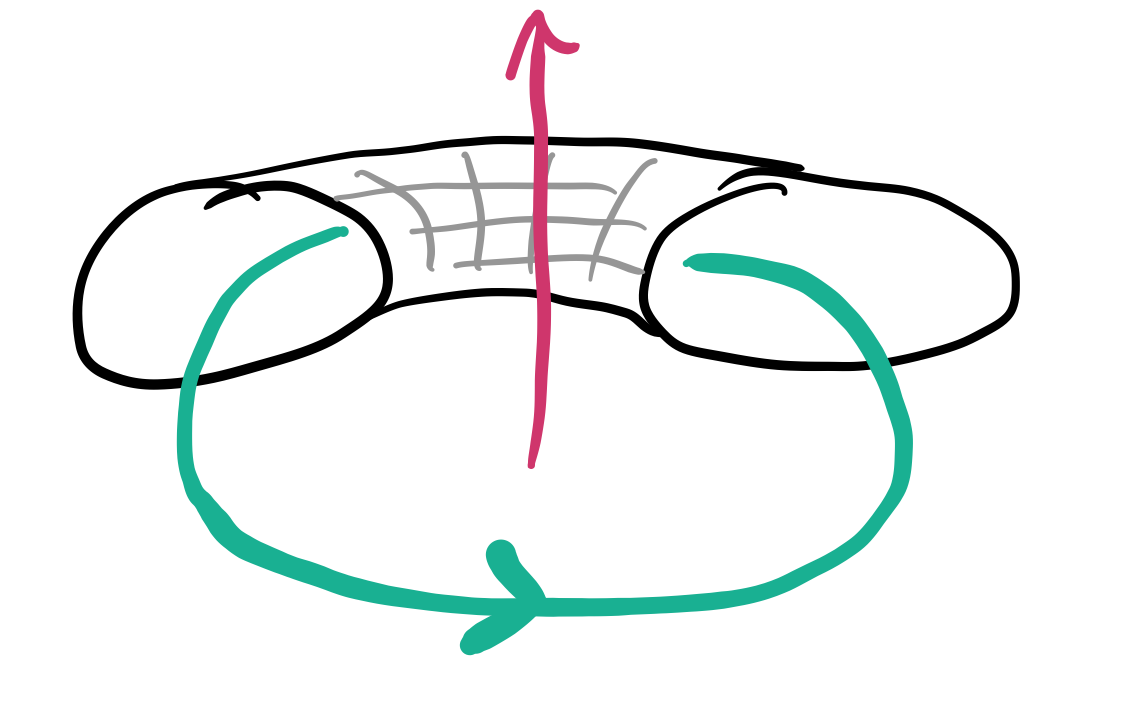
\includegraphics[width=0.57\textwidth,height=\textheight]{figure_code/amk_chapter/topological_fluxes.png}
\caption[{Topological Fluxes}]{Wilson loops that wind the major or minor diameters of the torus measure flux winding through the hole of the doughnut/torus or through the filling. If they made doughnuts that both had a jam filling and a hole, this analogy would be a lot easier to make \autocite{parkerWhyDoesThis}.}
\label{fig:topological_fluxes}
\end{figure}
}

However, in the non-Abelian phase we have to wrangle with monodromy \autocite{chungExplicitMonodromyMoore2007,oshikawaTopologicalDegeneracyNonAbelian2007}. Monodromy is the behaviour of objects as they move around a singularity. This manifests here in that the identity of a vortex and cloud of Majoranas can change as we wind them around the torus in such a way that, rather than annihilating to the vacuum, we annihilate them to create an excited state instead of a ground state. This means that we end up with only three degenerate ground states in the non-Abelian phase \((+1, +1), (+1, -1), (-1, +1)\) \autocite{chungTopologicalQuantumPhase2010,yaoAlgebraicSpinLiquid2009}. Concretely, this is because the projector enforces both flux and fermion parity. When we wind a vortex around both non-contractible loops of the torus, it flips the flux parity. Therefore, we have to introduce a fermionic excitation to make the state physical. Hence, the process does not give a fourth ground state.

Recently, the topology has notably gained interest because of proposals to use this ground state degeneracy to implement both passively fault tolerant and actively stabilised quantum computations \autocite{kitaevFaulttolerantQuantumComputation2003,poulinStabilizerFormalismOperator2005,hastingsDynamicallyGeneratedLogical2021}.

\begin{Shaded}
\begin{Highlighting}[]

\end{Highlighting}
\end{Shaded}

\hypertarget{amk-methods}{%
\section{Methods}\label{amk-methods}}

The practical implementation of what is described in this section is available as a Python package called Koala (Kitaev On Amorphous LAttices)~\autocite{hodsonKoalaKitaevAmorphous2022}. All results and figures were generated with Koala.

If we only care about the value of \(E_{u,0}\), it is possible to skip forming the fermionic operators. The eigenvalues obtained directly from diagonalising \(J^{\alpha} u_{ij}\) come in \(\pm \epsilon_m\) pairs. We can take half the absolute value of the whole set to recover \(\sum_m \epsilon_m\) easily.

\hypertarget{voronisation}{%
\subsection{Voronisation}\label{voronisation}}

To study the properties of the amorphous Kitaev model, we need to sample from the space of possible trivalent graphs.

A simple method is to use a Voronoi partition of the torus~\autocite{mitchellAmorphousTopologicalInsulators2018,marsalTopologicalWeaireThorpeModels2020,florescu_designer_2009}. We start by sampling \emph{seed points} uniformly (or otherwise) on the torus. Then, we compute the partition of the torus into regions closest (with a Euclidean metric) to each seed point. The straight lines (if the torus is flattened out) at the borders of these regions become the edges of the new lattice. The points where they intersect become the vertices.

The graph generated by a Voronoi partition of a two dimensional surface is always planar. This means that no edges cross each other when the graph is embedded into the plane. It is also trivalent in that every vertex is connected to exactly three edges \textbf{cite}.

Ideally, we would sample uniformly from the space of possible trivalent graphs. Indeed, there has been some work on how to do this using a Markov Chain Monte Carlo approach~\autocite{alyamiUniformSamplingDirected2016}. However, it does not guarantee that the resulting graph is planar, which we must ensure so that the edges can be 3-coloured.

In practice, we use a standard algorithm~\autocite{barberQuickhullAlgorithmConvex1996} from Scipy~\autocite{virtanenSciPyFundamentalAlgorithms2020} which computes the Voronoi partition of the plane. To compute the Voronoi partition of the torus, we take the seed points and replicate them into a repeating grid. This will be either 3x3 or, for very small numbers of seed points, 5x5. Then, we identify edges in the output to construct a lattice on the torus.

\hypertarget{fig:lattice_construction_animated}{%
\begin{figure}
\centering
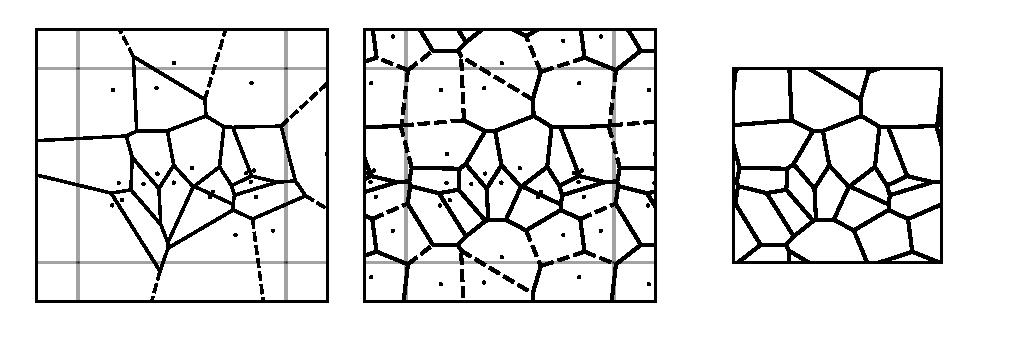
\includegraphics[width=1\textwidth,height=\textheight]{figure_code/amk_chapter/lattice_construction_animated/lattice_construction_animated}
\caption[{Lattice Construction}]{(Left) Lattice construction begins with the Voronoi partition of the plane with respect to a set of seed points (black points) sampled uniformly from \(\mathbb{R}^2\). (Center) However, we want the Voronoi partition of the torus, so we tile the seed points into a three by three grid. The boundaries of each tile are shown in light grey. (Right) Finally, we identify edges corresponding to each other across the boundaries to produce a graph on the torus. An edge colouring is shown here to help the reader identify corresponding edges. \href{http://thomashodson.com/assets/thesis/figure_code/amk_chapter/lattice_construction_animated/lattice_construction_animated.gif}{ Animated version online.}}
\label{fig:lattice_construction_animated}
\end{figure}
}

\hypertarget{graph-representation}{%
\subsection{Graph Representation}\label{graph-representation}}

Three keys pieces of information allow us to represent amorphous lattices.

Most of the graph connectivity is encoded by an ordered list of edges \((i,j)\). These are ordered to represent both directed and undirected graphs. This is useful for defining the sign of bond operators \(u_{ij} = - u_{ji}\).

Information about the embedding of the lattice onto the torus is encoded into a point on the unit square associated with each vertex. The torus is unwrapped onto the square by defining an arbitrary pair of cuts along the major and minor axes. For simplicity, we take these axes to be the lines \(x = 0\) and \(y = 0\). We can wrap the unit square back up into a torus by identifying the lines \(x = 0\) with \(x = 1\) and \(y = 0\) with \(y = 1\).

Finally, we need to encode the topology of the graph. This is necessary because, if we are simply given an edge \((i, j)\) we do not know how the edge gets from vertex i to vertex j. One method would be taking the shortest path, but it could also `go the long way around' by crossing one of the cuts. To encode this information, we store an additional vector \(\vec{r}\) associated with each edge. \(r_i^x = 0\) means that edge i does not cross the x. \(r_i^x = +1\) (\(-1\)) means it crossed the cut in a positive (negative) sense.

This description of the lattice has a very nice relationship to Bloch's theorem. Applying Bloch's theorem to a periodic lattice essentially means wrappping the unit cell onto a torus. Variations that happen at longer length scales than the size of the unit cell are captured by the crystal momentum. The crystal momentum inserts a phase factor \(e^{i \vec{q}\cdot\vec{r}}\) onto bonds that cross to adjacent unit cells. The vector \(\vec{r}\) is exactly what we use to encode the topology of our lattices.

\hypertarget{fig:bloch}{%
\begin{figure}
\centering
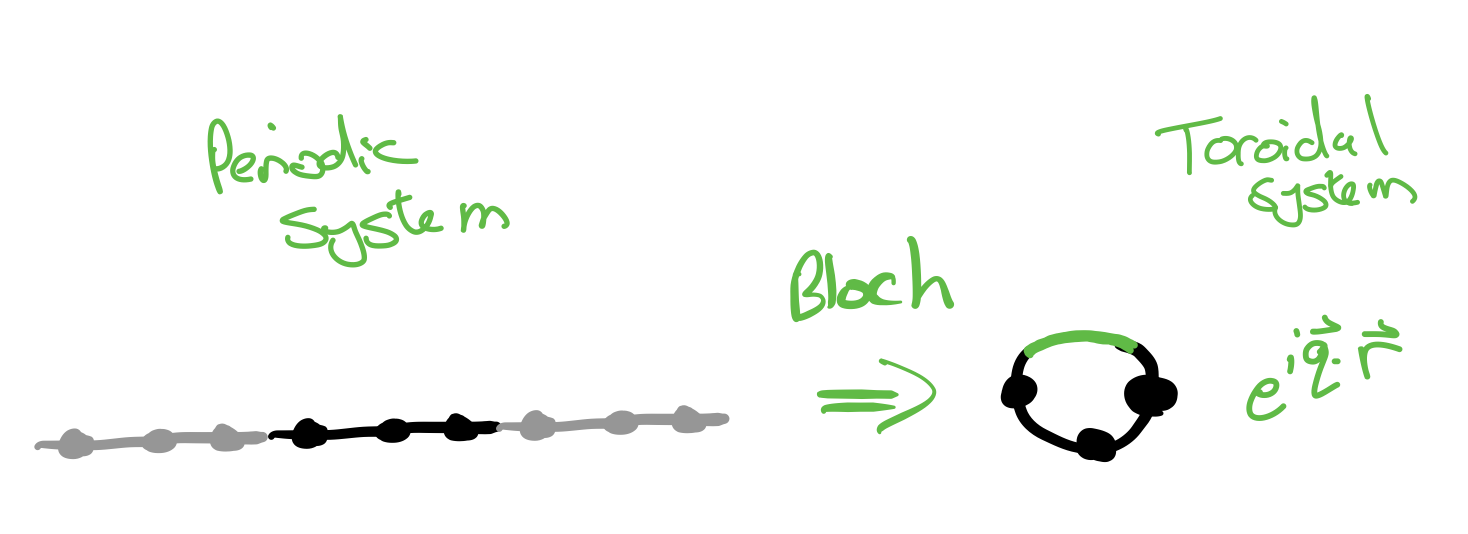
\includegraphics[width=1\textwidth,height=\textheight]{figure_code/amk_chapter/methods/bloch.png}
\caption[{Bloch's Theorem and the Torus}]{Bloch's theorem can be thought of as transforming from a periodic Hamiltonian on the place to the unit cell defined an torus. In addition we get some phase factors \(e^{i\vec{k}\cdot\vec{r}}\) associated with bonds that cross unit cells that depend on the sense in which they do so \(\vec{r} = (\pm1, \pm1)\). Representing graphs on the torus turns out to require a similar idea, we unwrap the torus to one unit cell and keep track of which bonds cross the cell boundaries.}
\label{fig:bloch}
\end{figure}
}

\hypertarget{colouring-the-bonds}{%
\subsection{Colouring the Bonds}\label{colouring-the-bonds}}

The Kitaev Model requires that each edge in the lattice be assigned a label \(x\), \(y\) or \(z\), such that each vertex has exactly one edge of each type connected to it. Let \(\Delta\) be the maximum degree of a graph which, in our case, is 3. If \(\Delta > 3\), it is obviously not possible to three-colour the edges. However, the general theory of when this is and is not possible for graphs with \(\Delta \leq 3\) is more subtle.

In the graph theory literature, graphs where all vertices have degree three are commonly called cubic graphs. There is no term for graphs with maximum degree three. Planar graphs are graphs which can be embedded onto the plane without any edges crossing. Bridgeless graphs do not contain any edges that, when removed, would partition the graph into disconnected components.

This problem must be distinguished from that considered by the famous four-colour theorem~\autocite{appelEveryPlanarMap1989}. The 4-colour theorem is concerned with assigning colours to the \textbf{vertices} of a graph, such that no vertices that share an edge have the same colour. Here we are concerned with an edge colouring.

The four-colour theorem applies to planar graphs, those that can be embedded onto the plane without any edges crossing. Here we are concerned with Toroidal graphs, which can be embedded onto the torus without any edges crossing. In fact, toroidal graphs require up to seven colours~\autocite{heawoodMapColouringTheorems}. The complete graph \(K_7\) is a good example of a toroidal graph that requires seven colours.

\(\Delta + 1\) colours are enough to edge-colour any graph. An \(\mathcal{O}(mn)\) algorithm exists to do it for a graph with \(m\) edges and \(n\) vertices~\autocite{gEstimateChromaticClass1964}. Restricting ourselves to graphs with \(\Delta = 3\) like ours, those can be four-edge-coloured in linear time~\autocite{skulrattanakulchai4edgecoloringGraphsMaximum2002}.

However, three-edge-colouring them is more difficult. Cubic, planar, bridgeless graphs can be three-edge-coloured if and only if they can be four-face-coloured~\autocite{tait1880remarks}. An \(\mathcal{O}(n^2)\) algorithm exists here~\autocite{robertson1996efficiently}. However, it is not clear whether this extends to cubic, \textbf{toroidal} bridgeless graphs.

\hypertarget{fig:multiple_colourings}{%
\begin{figure}
\centering
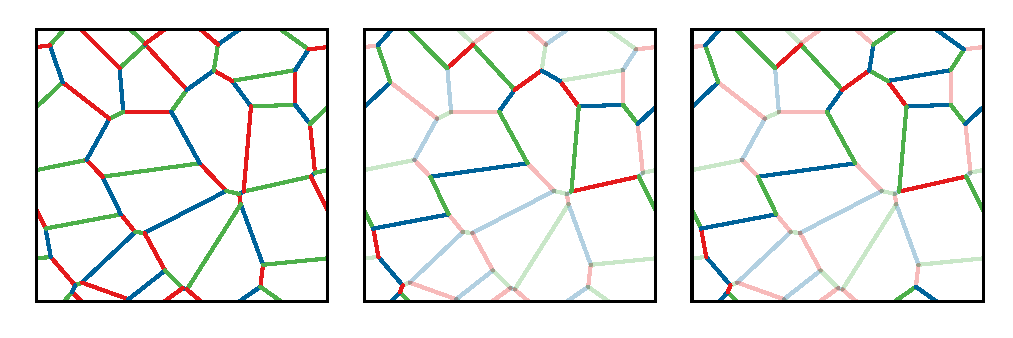
\includegraphics[width=1\textwidth,height=\textheight]{figure_code/amk_chapter/multiple_colourings/multiple_colourings}
\caption[{Colourings of an Amorphous Lattice}]{Three different valid 3-edge-colourings of amorphous lattices. Colors that differ from the leftmost panel are highlighted.}
\label{fig:multiple_colourings}
\end{figure}
}

\hypertarget{four-colourings-and-three-colourings}{%
\subsubsection{Four-colourings and three-colourings}\label{four-colourings-and-three-colourings}}

\textbf{add diagram of this}

A four-face-colouring can be converted into a three-edge-colouring quite easily: 1. Assume the faces of G can be four-coloured with labels (0,1,2,3) 2. Label each edge of G according to \(i + j \;\textrm{mod}\; 3\) where i and j are the labels of the face adjacent to that edge. For each edge label there are two face label pairs that do not share any face labels. i,e the edge label \(0\) can come about either from faces \(0 + 3\) or \(1 + 2\).

Explicitly, the mapping from face labels to edge labels is:

\[\begin{aligned}
0 + 3 \;\mathrm{or}\; 1 + 2 &= 0 \;\mathrm{mod}\; 3\\ 
0 + 1 \;\mathrm{or}\; 2 + 3 &= 1 \;\mathrm{mod}\; 3\\
0 + 2 \;\mathrm{or}\;1 + 3 &= 2 \;\mathrm{mod}\; 3\\
\end{aligned}
\]

\begin{enumerate}
\def\labelenumi{\arabic{enumi}.}
\setcounter{enumi}{2}
\item
  In a cubic planar G, a vertex v in G is always part of three faces and the colours of those faces determine the colours of the edges that connect to v. The three faces must take three distinct colours from the set \(\{0,1,2,3\}\).
\item
  From there, one can easily be convinced that those three distinct face colours can never produce repeated edge colours according to the \(i+j \;\mathrm{mod}\; 3\) rule.
\end{enumerate}

This implies that all cubic planar graphs are three-edge-colourable. This does not apply to toroidal graphs. We have not yet generated a Voronoi lattices on the torus that is not three-edge-colourable. This suggests that Voronoi lattices may have additional structures that make them three-edge-colourable. Intuitively, it seems that the kinds of toroidal graphs that cannot be three-edge-coloured could never be generated by a Voronoi partition with more than a few seed points.

\hypertarget{finding-lattice-colourings-with-minisat}{%
\subsubsection{Finding Lattice colourings with miniSAT}\label{finding-lattice-colourings-with-minisat}}

Some issues are harder in theory than in practice. Three-edge-colouring cubic toroidal graphs appears to be one of those things.

To find colourings, we use a Boolean Satisfiability Solver or SAT solver. A SAT problem is a set of statements about some number of boolean variables , such as ``\(x_1\) or not \(x_3\) is true'', and looks for an assignment \(x_i \in {0,1}\) that satisfies all the statements~\autocite{Karp1972}.

General purpose, high performance programs for solving SAT problems have been an area of active research for decades~\autocite{alounehComprehensiveStudyAnalysis2019}. Such programs are useful because, by the Cook-Levin theorem, any NP problem can be encoded in polynomial time as an instance of a SAT problem . This property is what makes SAT one of the subset of NP problems called NP-Complete~\autocite{cookComplexityTheoremprovingProcedures1971,levin1973universal}.

Thus, it is a relatively standard technique in the computer science community to solve NP problems by first transforming them to SAT instances and then using an off the shelf SAT solver. The output of this can then be mapped back to the original problem domain.

NP problems can be loosely considered as those which do not have a special structure than can be exploited to compute their solution in polynomial time. Our three-edge-colouring problem is likely not in NP. However, since we do not know what special structure it might have that could be used to speed up its solution, using a SAT solver appears to be a reasonable first method to try. As will be discussed later, this turned out to work well enough and looking for a better solution was not necessary.

We use a solver called \texttt{MiniSAT}~\autocite{imms-sat18}. Like most modern SAT solvers, \texttt{MiniSAT} requires the input problem to be specified in Conjunctive Normal Form (CNF). CNF requires that the constraints be encoded as a set of \emph{clauses} of the form \[x_1 \;\textrm{or}\; -x_3 \;\textrm{or}\; x_5\] that contain logical ORs of some subset of the variables where any of the variables may also be logically NOT'd, which we represent by negation here.

A solution of the problem is one that makes all the clauses simultaneously true.

We encode the edge colouring problem by assigning \(3B\) boolean variables to each of the \(B\) edges of the graph, \(x_{i\alpha}\) where \(x_{i\alpha} = 1\) indicates that edge \(i\) has colour \(\alpha\).

For edge colouring graphs we need two types of constraints: 1. Each edge is exactly one colour. 2. No neighbouring edges are the same colour.

The first constraint is a product of doing this mapping to boolean variables. The solver does not know anything about the structure of the problem unless it is encoded into the variables.

Let's say we have three variables that correspond to particular edge being red \(r\), green \(g\) or blue \(b\).

To require that exactly one of the variables be true, we can enforce that no pair of variables be true: \texttt{-(r\ and\ b)\ -(r\ and\ g)\ -(b\ and\ g)}

However, these clauses are not in CNF form. Therefore, we also have to use the fact that \texttt{-(a\ and\ b)\ =\ (-a\ OR\ -b)}. To enforce that at least one of these is true we simply OR them all together \texttt{(r\ or\ b\ or\ g)}

To encode the fact that no adjacent edges can have the same colour, we emit a clause that, for each pair of adjacent edges, they cannot be both red, both green or both blue.

We get a solution or set of solutions from the solver, which we can map back to a labelling of the edges. \cref{fig:multiple_colourings} shows some examples.

The solution presented here works well enough for our purposes. It does not take up a substantial fraction of the overall computation time, see +fig:times but other approaches could likely work.

When translating problems to CNF form, there is often some flexibility. For instance, we used three boolean variables to encode the colour of each edge and, then, additional constraints to require that only one of these variables be true. An alternative method which we did not try would be to encode the label of each edge using two variables, yielding four states per edge, and then add a constraint that one of the states, say (true, true) is disallowed. This would, however, have added some complexity to the encoding of the constraint that no adjacent edges can have the same colour.

The popular \emph{Networkx} Python library uses a greedy graph colouring algorithm. It simply iterates over the vertices/edges/faces of a graph and assigns them a colour that is not already disallowed. This does not work for our purposes because it is not designed to look for a particular n-colouring. However, it does include the option of using a heuristic function that determine the order in which vertices will be coloured~\autocite{kosowski2004classical,matulaSmallestlastOrderingClustering1983}. Perhaps

\hypertarget{fig:times}{%
\begin{figure}
\centering
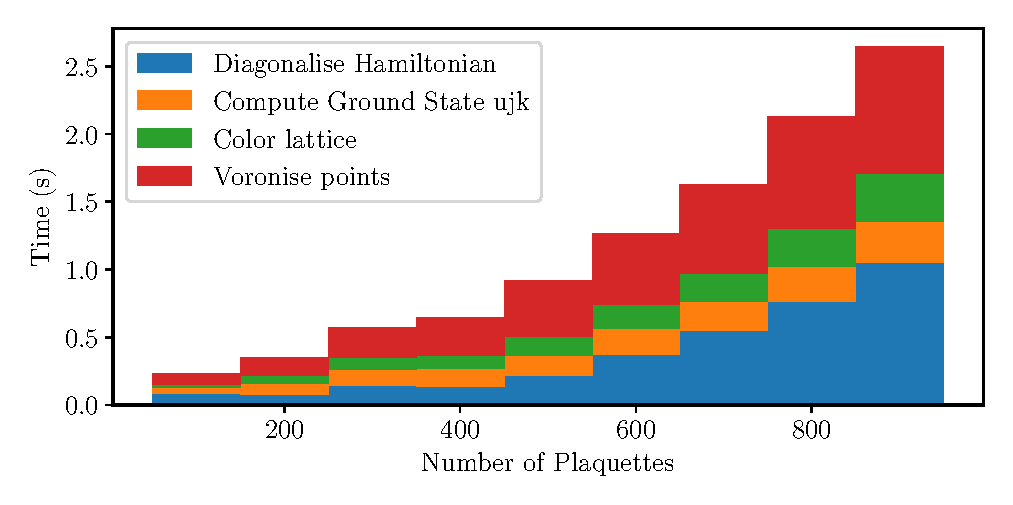
\includegraphics[width=1\textwidth,height=\textheight]{figure_code/amk_chapter/methods/times/times}
\caption[{Computation Time Spent on Different Procedures.}]{The proportion of computation time taken up by the four longest running steps when generating a lattice. For larger systems, the time taken to perform the diagonalisation dominates.}
\label{fig:times}
\end{figure}
}

\hypertarget{does-it-matter-which-colouring-we-choose}{%
\subsubsection{Does it matter which colouring we choose?}\label{does-it-matter-which-colouring-we-choose}}

In the isotropic case \(J^\alpha = 1\), it is easy to show that choosing a particular valid colouring cannot make a difference. As the choice of how we define the four Majoranas at a site is arbitrary, we can define a local operator that transforms the colouring of any particular site to another permutation. The operators commute with the Hamiltonian and, by composing such operators, we can transform the Hamiltonian generated by one colouring into that generated by another.

We cannot do this in the anisotropic case. It remains an open question whether particular physical properties could arise by engineering the colouring in this phase though we expect them to exhibit a self averaging behaviour.

\hypertarget{mapping-between-flux-sectors-and-bond-sectors}{%
\subsection{Mapping between flux sectors and bond sectors}\label{mapping-between-flux-sectors-and-bond-sectors}}

Constructing the Majorana representation of the model requires the particular bond configuration \(u_{jk} = \pm 1\). However, the large number of gauge symmetries of the bond sector makes it unwieldy to work with. Therefore, we need a way to quickly map between bond sectors and flux sectors.

Going from the bond sector to flux sector is easy. We can compute it directly by taking the product of \(i u_{jk}\) around each plaquette \[ \phi_i = \prod_{(j,k) \; \in \; \partial \phi_i} i u_{jk}\]

Going from flux sector to bond sector requires more thought. The algorithm we use is this:

\begin{enumerate}
\def\labelenumi{\arabic{enumi}.}
\item
  Fix the gauge by choosing some arbitrary \(u_{jk}\) configuration. In practice, we use \(u_{jk} = +1\). This chooses an arbitrary one of the four topological sectors.
\item
  Compute the current flux configuration and how it differs from the target one. We refer to a plaquette that differs from the target as a ``defect''.
\item
  Find any adjacent pairs of defects and flip the \(u_jk\) between them. This leaves a set of isolated defects.
\item
  Pair the defects up using a greedy algorithm.
\item
  Compute paths along the dual lattice between each pair of plaquettes. Flipping the corresponding set of bonds transports one flux to the other and annihilates them.
\end{enumerate}

\hypertarget{fig:flux_finding}{%
\begin{figure}
\centering
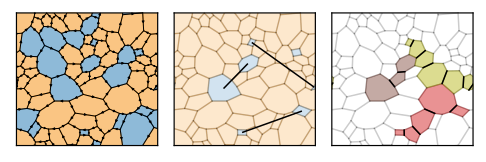
\includegraphics[width=1\textwidth,height=\textheight]{figure_code/amk_chapter/flux_finding/flux_finding}
\caption[{Finding Bond Sectors from Flux Sectors}]{(Left) The ground state flux sector and bond sector for an amorphous lattice. Bond arrows indicate the direction in which \(u_{jk} = +1\). Plaquettes are coloured blue when \(\hat{\phi}_i = -1\) (\(-i\)) for even/odd plaquettes and orange when \(\hat{\phi}_i = +1\) (\(+i\)) for even/odd plaquettes. (Centre) To transform this to the target flux sector (all \(+1\)/\(+i\)), we first flip any \(u_{jk}\) that are between two fluxes. This leaves a set of isolated fluxes that must be annihilated. Then, these are paired up as indicated by the black lines. (Right) A* search is used to find paths (coloured plaquettes) on the dual lattice between each pair of fluxes and the corresponding \(u_{jk}\) (shown in black) are flipped. One flux will remain because the starting and target flux sectors differed by an odd number of fluxes.}
\label{fig:flux_finding}
\end{figure}
}

\hypertarget{chern-markers}{%
\subsection{Chern Markers}\label{chern-markers}}

We know that the standard Kitaev model supports both Abelian and non-Abelian phases. Therefore, how can we assess whether this is also the case for the amorphous Kitaev model?

We have already discussed the fact that topology and anyonic statistics are intimately linked. This will help here. The Chern number is a quantity that measures the topological characteristics of a material.

The original definition of the Chern number relies on the model having translation symmetry. This leads to the development of \emph{local markers}. These are operators that generalise the notion of the Chern number to an observable over some region smaller than the entire system.

\textbf{Expand on definition here}

\textbf{Discuss link between Chern number and Anyonic Statistics}

\hypertarget{amk-results}{%
\section{Results}\label{amk-results}}

This section contains our results on the AK model, we first look at how we checked numerically that Lieb's theorem generalises to our model. Next we compute the ground state diagram and look at the two phases that arise there. We then use a local Chern marker and the presence of edge modes to characterise these phases as having Abelian or non-Abelian statistics. Finally we look at the finite temperature behaviour of the model.

\hypertarget{the-ground-state-flux-sector}{%
\subsection{The Ground State Flux Sector}\label{the-ground-state-flux-sector}}

We will check that Lieb's theorem generalises to our model by enumerating all the flux sectors of many separate amorphous lattice realisations. However we have two seemingly irreconcilable problems. Finite size effects have a large energetic contribution for small systems~\autocite{kitaevAnyonsExactlySolved2006} so we would like to perform our analysis for very large lattices. However for an amorphous system with \(N\) plaquettes, \(2N\) edges and \(3N\) vertices we have \(2^{N-1}\) flux sectors to check and diagonalisation scales with \(\mathcal{O}(N^3)\). That exponential scaling makes it difficult to work with lattices much larger than \(16\) plaquettes with the resources.

To get around this we instead look at periodic systems with amorphous unit cells. For a similarly sized periodic system with \(A\) unit cells and \(B\) plaquettes in each unit cell where \(N \sim AB\) things get much better. We can use Bloch's theorem to diagonalise this system in about \(\mathcal{O}(A B^3)\) operations, and more importantly there are only \(2^{B-1}\) flux sectors to check. We fully enumerated the flux sectors of \(\sim\) 25,000 periodic systems with disordered unit cells of up to \(B = 16\) plaquettes and \(A = 100\) unit cells. However, showing that our guess is correct for periodic systems with disordered unit cells is not quite convincing on its own as we have effectively removed longer-range disorder from our lattices.

The second part of the argument is to show that the energetic effect of introducing periodicity scales away as we go to larger system sizes and has already diminished to a small enough value at 16 plaquettes, which is indeed what we find. From this we argue that the results for small periodic systems generalise to large amorphous systems. In the isotropic case (\(J^\alpha = 1\)), Lieb's theorem correctly predicts the ground state flux sector for all of the lattices we tested. For the toric code phase (\(J^x = J^y = 0.25, J^z = 1\)) all but around (\(\sim 0.5 \%\)) lattices had ground states conforming to our conjecture. In these cases, the energy difference between the true ground state and our prediction was on the order of \(10^{-6} J\).

The spin Kitaev Hamiltonian is real and therefore has time reversal symmetry. However in the ground state the flux \(\phi_p\) through any plaquette with an odd number of sides has imaginary eigenvalues \(\pm i\). Thus, states with a fixed flux sector spontaneously break time reversal symmetry. Kiteav noted this in his original paper but it was first explored in a concrete model by Yao and Kivelson~for a translation invariant Kitaev model with odd sided plaquettes~\autocite{Yao2011}.

Flux sectors come in degenerate pairs, where time reversal is equivalent to inverting the flux through every odd plaquette, a general feature for lattices with odd plaquettes~\autocite{yaoExactChiralSpin2007,Peri2020}. This spontaneously broken symmetry serves a role analogous to the external magnetic field in the original honeycomb model, leading the AK model to have a non-Abelian anyonic phase without an external magnetic field.

\hypertarget{ground-state-phase-diagram}{%
\subsection{Ground State Phase Diagram}\label{ground-state-phase-diagram}}

The triangular \(J_x, J_y, J_z\) phase diagram of this family of models arises from setting the energy scale with \(J_x + J_y + J_z = 1\). The intersection of this plane and the unit cube is what yields the equilateral triangles seen in diagrams like \cref{fig:phase_diagram}. The KH model has an Abelian, gapped phase in the anisotropic region (the A phase) and is gapless in the isotropic region. The introduction of a magnetic field breaks the chiral symmetry, leading to the isotropic region becoming a gapped, non-Abelian phase, the B phase.

Similar to the KH model with a magnetic field, we find that the amorphous model is only gapless along critical lines, see \cref{fig:phase_diagram} (Left). Interestingly, in finite size systems the gap closing exists in only one of the four topological sectors though the sectors become degenerate in the thermodynamic limit. Nevertheless this could be a useful way to define the (0, 0) topological flux sector for the amorphous model which otherwise has no natural way to choose it.

In the honeycomb model, the phase boundaries are located on the straight lines \(|J^x| = |J^y| \;+ \;|J^z|\) and permutations of \(x,y,z\). These are shown as dotted lines in \cref{fig:phase_diagram} (Right). We find that on the amorphous lattice these boundaries exhibit an inward curvature, similar to honeycomb Kitaev models with flux or bond disorder~\autocite{knolle_dynamics_2016,Nasu_Thermal_2015,lahtinenPerturbedVortexLattices2014,willansDisorderQuantumSpin2010,zschockePhysicalStatesFinitesize2015,kaoDisorderDisorderLocalization2021}.

\hypertarget{fig:phase_diagram}{%
\begin{figure}
\centering
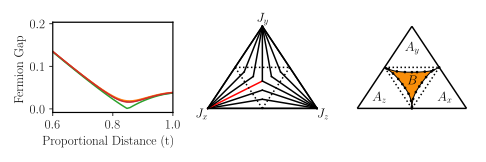
\includegraphics[width=1\textwidth,height=\textheight]{figure_code/amk_chapter/results/phase_diagram/phase_diagram}
\caption[{The Ground State Phase Diagram}]{The phase diagram of the model can be characterised by an equilateral triangle whose corners indicate points where \(J_\alpha = 1, J_\beta = J_\gamma = 0\) while the centre denotes \(J_x = J_y = J_z\). (Center) To compute critical lines efficiently in this space we evaluate the order parameter of interest along rays shooting from the corners of the phase diagram. The ray highlighted in red defines the values of J used for the left figure. (Left) The fermion gap as a function of J for an amorphous system with 20 plaquettes, where the x axis is the position on the red line in the central figure from 0 to 1. For finite size systems the four topological sectors are not degenerate and only one of them (in green) has a true gap closing. (Right) The Abelian \(A_\alpha\) phases of the model and the non-Abelian B phase separated by critical lines where the fermion gap closes. Later we will show that the Chern number \(\nu\) changes from \(0\) to \(\pm 1\) from the A phases to the B phase. Indeed the gap \emph{must} close in order for the Chern number to change~\autocite{ezawaTopologicalPhaseTransition2013}.}
\label{fig:phase_diagram}
\end{figure}
}

\hypertarget{abelian-or-non-abelian-statistics-of-the-gapped-phase}{%
\subsubsection{Abelian or non-Abelian statistics of the Gapped Phase}\label{abelian-or-non-abelian-statistics-of-the-gapped-phase}}

The two phases of the amorphous model are gapped as we can see from the finite size scaling of \cref{fig:fermion_gap_vs_L}. The next question is: do these phases support excitations with trivial, Abelian or non-Abelian statistics? To answer that we turn to Chern numbers~\autocite{berryQuantalPhaseFactors1984,simonHolonomyQuantumAdiabatic1983,thoulessQuantizedHallConductance1982}. As discussed earlier the Chern number is a quantity intimately linked to both the topological properties and the anyonic statistics of a model. Here we will make use of the fact that the Abelian/non-Abelian character of a model is linked to its Chern number~\autocite{kitaevAnyonsExactlySolved2006}. The Chern number is only defined for the translation invariant case so we instead use a family of real space generalisations of the Chern number that work for amorphous systems called local topological markers~\autocite{bianco_mapping_2011,Hastings_Almost_2010,mitchellAmorphousTopologicalInsulators2018}.

There are many possible choices here, indeed Kitaev defines one in his original paper on the KH model~\autocite{kitaevAnyonsExactlySolved2006}. Here we use the crosshair marker of~\autocite{peru_preprint} because it works well on smaller systems. We calculate the projector \(P = \sum_i |\psi_i\rangle \langle \psi_i|\) onto the occupied fermion eigenstates of the system in open boundary conditions. The projector encodes local information about the occupied eigenstates of the system and in gapped systems it is exponentially localised~\autocite{hastingsLiebSchultzMattisHigherDimensions2004}. The name \emph{crosshair} comes from the fact that the marker is defined with respect to a particular point \((x_0, y_0)\) by step functions in x and y

\[\begin{aligned}
    \nu (x, y) = 4\pi \; \Im\; \mathrm{Tr}_{\mathrm{B}} 
    \left ( 
    \hat{P}\;\hat{\theta}(x-x_0)\;\hat{P}\;\hat{\theta}(y-y_0)\; \hat{P}
    \right ),
\end{aligned}\]

when the trace is taken over a region \(B\) around \((x_0, y_0)\) that is large enough to include local information about the system but does not come too close to the edges. If these conditions are met then then this quantity will be very close to quantised to the Chern number, see \cref{fig:phase_diagram_chern}. We'll use the crosshair marker to assess the Abelian/non-Abelian character of the phases.

In the A phase of the amorphous model we find that \(\nu=0\) and hence the excitations have Abelian character, similar to the honeycomb model. This phase is thus the amorphous analogue of the Abelian toric-code QSL~\autocite{kitaev_fault-tolerant_2003}. The B phase has \(\nu=\pm1\) so is a non-Abelian Chiral Spin Liquid (CSL) similar to that of the Yao-Kivelson model~\autocite{yaoExactChiralSpin2007}. The CSL state is the magnetic analogue of the fractional quantum Hall state~\autocite{laughlinPropertiesChiralspinliquidState1990}. Hereafter we focus our attention on this phase.

\hypertarget{fig:phase_diagram_chern}{%
\begin{figure}
\centering
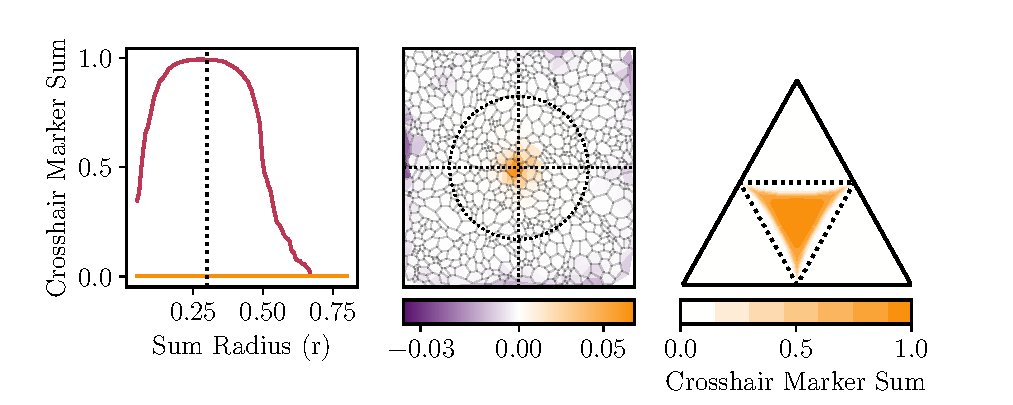
\includegraphics[width=1\textwidth,height=\textheight]{figure_code/amk_chapter/results/phase_diagram_chern/phase_diagram_chern}
\caption[{Local Chern Markers}]{(Center) The crosshair marker~\autocite{peru_preprint}, a local topological marker, evaluated on the Amorphous Kitaev model. The marker is defined around a point, denoted by the dotted crosshair. Information about the local topological properties of the system are encoded within a region around that point. (Left) Summing these contributions up to some finite radius (dotted line here, dotted circle in the centre) gives a generalised version of the Chern number for the system which becomes quantised in the thermodynamic limit. The radius must be chosen large enough to capture information about the local properties of the lattice while not so large as to include contributions from the edge states. The isotropic regime \(J_\alpha = 1\) in red has \(\nu = \pm 1\) implying it supports excitations with non-Abelian statistics, while the anisotropic regime in orange has \(\nu = 0\) implying Abelian statistics. (Right) Extending this analysis to the whole \(J_\alpha\) phase diagram with fixed \(r = 0.3\) nicely confirms that the isotropic phase is non-Abelian.}
\label{fig:phase_diagram_chern}
\end{figure}
}

\hypertarget{edge-modes}{%
\subsubsection{Edge Modes}\label{edge-modes}}

Chiral Spin Liquids support topological protected edge modes on open boundary conditions~\autocite{qi_general_2006}. \Cref{fig:edge_modes} shows the probability density of one such edge mode. It is near zero energy and exponentially localised to the boundary of the system. While the model is gapped in periodic boundary conditions (i.e on the torus) these edge modes appear in the gap when the boundary is cut.

The localisation of the edge modes can be quantified by their inverse participation ratio (IPR) and its scaling with system size \(\tau\), \[\mathrm{IPR} = \int d^2r|\psi(\mathbf{r})|^4  \propto L^{-\tau},\] where \(L\sim\sqrt{N}\) is the linear dimension of the amorphous lattices. This is relevant because localised in-gap states do not participate in transport and hence do not turn band insulators into conductive metals. It is only when the gap fills with extended states that we get a conductive state.

\hypertarget{fig:edge_modes}{%
\begin{figure}
\centering
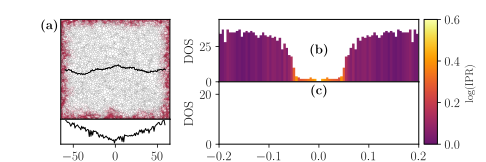
\includegraphics[width=1\textwidth,height=\textheight]{figure_code/amk_chapter/results/edge_modes/edge_modes}
\caption[{Edges States and Density of States}]{(a) The density of one of the topologically protected edge states in the B phase. (Below) the log density plotted along the black path showing that the state is exponentially localised. (a)/(b) The density of states of the corresponding lattice in (a) periodic boundary conditions, (b) open boundary conditions. The colour of the bars shows the mean log IPR for each energy window. Cutting the boundary fills the gap with localised states.}
\label{fig:edge_modes}
\end{figure}
}

\hypertarget{anderson-transition-to-a-thermal-metal}{%
\subsection{Anderson Transition to a Thermal Metal}\label{anderson-transition-to-a-thermal-metal}}

\hypertarget{fig:fermion_gap_vs_L}{%
\begin{figure}
\centering
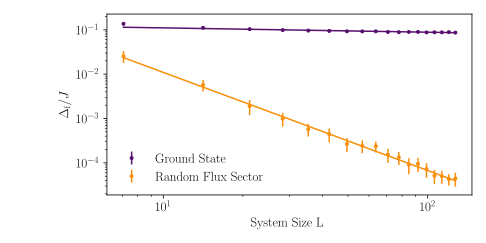
\includegraphics[width=1\textwidth,height=\textheight]{figure_code/amk_chapter/results/fermion_gap_vs_L/fermion_gap_vs_L}
\caption[{Finite Size Scaing of the Fermion Gap}]{Within a flux sector, the fermion gap \(\Delta_f\) measures the energy between the fermionic ground state and the first excited state. This graph shows the fermion gap as a function of system size for the ground state flux sector and for a configuration of random fluxes. We see that the disorder induced by an putting the Kitaev model on an amorphous lattice does not close the gap in the ground state. The gap closes in the flux disordered limit is good evidence that the system transitions to a gapless thermal metal state at high temperature. Each point shows an average over 100 lattice realisations. System size \(L\) is defined \(\sqrt{N}\) where N is the number of plaquettes in the system. Error bars shown are \(3\) times the standard error of the mean. The lines shown are fits of \(\tfrac{\Delta_f}{J} = aL ^ b\) with fit parameters: Ground State: \(a = 0.138 \pm 0.002, b = -0.0972 \pm 0.004\) Random Flux Sector: \(a = 1.8 \pm 0.2, b = -2.21 \pm 0.03\)}
\label{fig:fermion_gap_vs_L}
\end{figure}
}

Previous work on the honeycomb model at finite temperature has shown that the B phase undergoes a thermal transition from a QSL phase to a \emph{thermal metal} phase~\autocite{selfThermallyInducedMetallic2019}. This happens because at finite temperature, thermal fluctuations excite spontaneous vortex-pair formation. As discussed previously, these fluxes are dressed by Majorana bounds states and the composite object is an Ising-type non-Abelian anyon~\autocite{Beenakker2013}. The interactions between these anyons are oscillatory, similar to the Ruderman-Kittel-Kasuya-Yosida (RKKY) exchange and decay exponentially with separation~\autocite{Laumann2012,Lahtinen_2011,lahtinenTopologicalLiquidNucleation2012}. At sufficient density, the anyons hybridise to a macroscopically degenerate state known as \emph{thermal metal}~\autocite{Laumann2012}. At close range the oscillatory behaviour of the interactions can be modelled by a random sign which forms the basis for a random matrix theory description of the thermal metal state.

The amorphous chiral spin liquid undergoes the same Anderson transition to a thermal metal state. Markov Chain Monte Carlo would be necessary to simulate this in full detail~\autocite{selfThermallyInducedMetallic2019} but in order to avoid that complexity in the current work we instead opted to use vortex density \(\rho\) as a proxy for temperature. We give each plaquette the probability \(\rho\) of being a vortex, possibly with one additional adjustment to preserve overall vortex parity. This approximation is exact in the limits \(T = 0\) (corresponding to \(\rho = 0\)) and \(T \to \infty\) (corresponding to \(\rho = 0.5\)) while at intermediate temperatures there may be vortex-vortex correlations that are not captured by our uncorrelated vortex placement.

First we performed a finite size scaling to check that the presence of a gap in the CSL ground state and absence of a gap in the thermal metal phase are both robust as we go to larger systems, see \cref{fig:fermion_gap_vs_L}. Next we evaluated the fermionic density of states (DOS), Inverse Participation Ratio and IPR scaling exponent \(\tau\) as functions of the vortex density \(\rho\), see \cref{fig:DOS_vs_rho}. This leads to a nice picture of what happens as we raise the temperature of the system away from the gapped, insulating CSL phase. At small \(\rho\), states begin to populate the gap but they have \(\tau\approx0\), indicating that they are localised states pinned to the vortices, and the system remains insulating. At large \(\rho\), the in-gap states merge with the bulk band and become extensive, closing the gap, and the system transitions to the thermal metal phase.

\hypertarget{fig:DOS_vs_rho}{%
\begin{figure}
\centering
\includegraphics[width=1\textwidth,height=\textheight]{figure_code/amk_chapter/results/DOS_vs_rho/DOS_vs_rho}
\caption[{Transition to a Thermal Metal}]{(Top) Density of states and (Bottom) scaling exponent \(\tau\) of the amorphous Kitaev model as a vortex density \(\rho\) is increased. The scaling exponent \(\tau\) is the exponent with which the inverse participation ratio scales with system size. It gives a measure of the degree of localisation of the states in each \((E/J, \rho)\) bin. At zero \(\rho\) we have the gapped ground state. At small \(\rho\), states begin to populate the gap. These states have \(\tau\approx0\), indicating that they are localised states pinned to fluxes, and the system remains insulating. As \(\rho\) increases further, the in-gap states merge with the bulk band and become extensive, fully closing the gap, and the system transitions to a thermal metal phase.}
\label{fig:DOS_vs_rho}
\end{figure}
}

The thermal metal phase has a signature logarithmic divergence at zero energy and oscillations in the DOS. These signatures can be shown to occur by a recursive argument that involves mapping the original model onto a Majorana model with interactions that take random signs which can itself be mapped onto a coarser lattice with lower energy excitations and so on. This can be repeating indefinitely, showing the model must have excitations at arbitrarily low energies in the thermodynamic limit~\autocite{bocquet_disordered_2000,selfThermallyInducedMetallic2019}. These signatures are shown in \cref{fig:DOS_oscillations} for our model and for the KH model. They do not occur in the KH model unless the chiral symmetry is broken by a magnetic field.

\hypertarget{fig:DOS_oscillations}{%
\begin{figure}
\centering
\includegraphics[width=1\textwidth,height=\textheight]{figure_code/amk_chapter/results/DOS_oscillations/DOS_oscillations}
\caption[{Distinctive Oscillations in the Density of States}]{Density of states at high temperature showing the logarithmic divergence at zero energy and oscillations characteristic of the thermal metal state~\autocite{bocquet_disordered_2000,selfThermallyInducedMetallic2019}. (a) shows the honeycomb lattice model in the B phase with magnetic field, while (b) shows that our model transitions to a thermal metal phase without an external magnetic field but rather due to the spontaneous chiral symmetry breaking. In both plots the density of vortices is \(\rho = 0.5\) corresponding to the \(T = \infty\) limit.}
\label{fig:DOS_oscillations}
\end{figure}
}

\hypertarget{sec:AMK-Conclusion}{%
\section{Discussion and Conclusion}\label{sec:AMK-Conclusion}}

In this chapter we have looked at an extension of the KH model to amorphous lattices with coordination number three. We discussed a method to construct arbitrary trivalent lattices using Voronoi partitions, how to embed them onto the torus and how to edge-colour them using a SAT solver. We showed numerically that the ground state flux sector of the model is given by a simple extension of Lieb's theorem. The model has two gapped QSL phases. The two phases support excitations with different anyonic statistics, Abelian and non-Abelian, distinguished using a real-space generalisation of the Chern number~\autocite{peru_preprint}. The presence of odd-sided plaquettes in the model resulted in spontaneous breaking of time reversal symmetry, leading to the emergence of a chiral spin liquid phase. Finally we showed evidence that the amorphous system undergoes an Anderson transition to a thermal metal phase, driven by the proliferation of vortices with increasing temperature. The AK model is an exactly solvable model of the chiral QSL state, one of the first models to exhibit a topologically non-trivial quantum many-body phase on an amorphous lattice. As such this study provides a number of future lines of research.

\hypertarget{experimental-realisations-and-signatures}{%
\subsubsection{Experimental Realisations and Signatures}\label{experimental-realisations-and-signatures}}

We should consider whether a physical amorphous system that supports a QSL ground state could exist. The search for translation invariant Kitaev systems is already motivated by the prospect of a physically realised QSL state, Majorana fermions and direct access to a system with emergent \(\mathbb{Z}_2\) gauge physics~\autocite{TrebstPhysRep2022}. An amorphous Kitaev model would provide all this and in addition the possibility of exploring the CSL state and potentially very different routes to a physical realisation. One route would be to ask if any crystalline Kitaev material candidates can be heated and rapidly quenched~\autocite{Weaire1976,Petrakovski1981,Kaneyoshi2018} to produce amorphous analogues that might preserve enough of their local structure to support a QSL state.

Considering more designer materials, metal organic frameworks (MOFs) could present a platform for a synthetic Kitaev material. These materials are composed of repeating units of large organic molecules coordinated with metal ions. Amorphous MOFs can be generated with mechanical processes that introduce disorder into crystalline MOFs~\autocite{bennett2014amorphous} and there have been recent proposals for realising strong Kitaev interactions~\autocite{yamadaDesigningKitaevSpin2017} in them as potential signatures of a resonating valence bond QSL state in MOFs with Kagome geometry~\autocite{misumiQuantumSpinLiquid2020}. Finally, MOFs are composed of large synthetic molecules so may provide more opportunity for fine tuning to target particular physics than with ionic compounds. There have also been proposals to realise Kitaev physics in optical lattice experiments~\autocite{duanControllingSpinExchange2003,micheliToolboxLatticespinModels2006} which can also support amorphous lattices~\autocite{sadeghiAmorphousTwodimensionalOptical2005}.

A physical realisation in either an amorphous compound or a MOF would likely entail a high degree of defects. Amorphous silicon, for instance, tends to contain dangling bonds which must be passivated by hydrogenation to improve its physical properties~\autocite{streetHydrogenatedAmorphousSilicon1991}. In both cases, if we assume that Kitaev physics can be realised by crystalline systems, it is not clear if the necessary superexchange couplings would survive the addition of disorder to the lattice. It would therefore make sense theoretically to examine how robust the CSL ground state of the AK model is to additional disorder in the Hamiltonian, for example mis-colourings of the bonds, vertex degree disorder and disorder in coupling strengths. Relatedly, one could look at perturbations to the Hamiltonian that break integrability~\autocite{Rau2014,Chaloupka2010,Chaloupka2013,Chaloupka2015,Winter2016}.

Considering experimental signatures, we expect that the chiral amorphous QSL will display a half-quantised thermal Hall effect similar to the magnetic field induced behaviour of KH materials~\autocite{Kasahara2018,Yokoi2021,Yamashita2020,Bruin2022}. Alternatively, the CSL state could be characterised by local probes such as spin-polarised scanning tunnelling microscopy~\autocite{Feldmeier2020,Konig2020,Udagawa2021} while the thermal metal phase displays characteristic longitudinal heat transport signatures~\autocite{Beenakker2013}. Local perturbations, such as those that might come from an atomic force microscope, could potentially be used to create and control vortices~\autocite{jangVortexCreationControl2021}. To this end it one could look at how the move to amorphous lattices affects vortex time dynamics in perturbed KH models~\autocite{joyDynamicsVisonsThermal2022}.

Given the lack of unambiguous signatures of the QSL state, it can be hard to distinguish the effects of the QSL state from the effect of disorder. So introducing topological disorder may only increase the experimental challenges. That being said, the presence of topological disorder may suppress competing interactions that would otherwise induce magnetic ordering at zero temperature potentially widening the class of materials that could host a QSL ground state. Alternatively, 3D realisations of the AK model could get around this issue of confusing a QSL with disorder because 3D would be expected to have a true Finite-Temperature Phase Transition (FTPT) to the thermal metal state that could be a useful experimental signature~\autocite{eschmannThermodynamicClassificationThreedimensional2020,OBrienPRB2016}. 3D Kitaev systems can also support CSL ground states~\autocite{mishchenkoChiralSpinLiquids2020}.

\hypertarget{thermodynamics}{%
\subsubsection{Thermodynamics}\label{thermodynamics}}

The KH model can be extended to 3D either on trivalent lattices~\autocite{eschmannThermodynamicClassificationThreedimensional2020,OBrienPRB2016} or it can be generalised to an exactly solvable spin-\(\tfrac{3}{2}\) model on 3D four-coordinate lattices~\autocite{yaoAlgebraicSpinLiquid2009,wenQuantumOrderStringnet2003,ryuThreedimensionalTopologicalPhase2009,Baskaran2008,Nussinov2009,Yao2011,Chua2011,Natori2020,Chulliparambil2020,Chulliparambil2021,Seifert2020,WangHaoranPRB2021,Wu2009}. In~\autocite{yaoAlgebraicSpinLiquid2009}, the 2D square lattice with 4 bond types (\(J_w, J_x, J_y, J_z\)) is considered. Since Voronoi partitions in 3D produce lattices of degree four, one interesting generalisation of this work would be to look at the spin-\(\tfrac{3}{2}\) Kitaev model on amorphous lattices.

We did not perform a full Markov Chain Monte Carlo (MCMC) simulation of the AK model at finite temperature but the possible extension to a 3D model with an FTPT would motivate this full analysis. This MCMC simulation would be a numerically challenging task but poses no conceptual barriers~\autocite{Laumann2012,lahtinenTopologicalLiquidNucleation2012,selfThermallyInducedMetallic2019}. Doing this would, first, allow one to look for possible violations of the Harris criterion~\autocite{harrisEffectRandomDefects1974} for the Ising transition of the flux sector. Recall that topological disorder in 2D has radically different properties to that of other kinds of disorder due to the constraints imposed by the Euler equation and maintaining coordination number which allows it to violate otherwise quite general rules like the Harris criterion~\autocite{barghathiPhaseTransitionsRandom2014,schrauthViolationHarrisBarghathiVojtaCriterion2018}. Second, incorporating the projector in addition to MCMC would allow for a full investigation of whether the effect of topological degeneracy is apparent at finite temperatures, this is done for the KH model in~\autocite{selfThermallyInducedMetallic2019}.

Next, one could investigate whether a QSL phase may exist for other models defined on amorphous lattices with a view to more realistic prospects of observation. Do the properties of the Kitaev-Heisenberg model generalise from the honeycomb to the amorphous case?~\autocite{Chaloupka2010,Chaloupka2015,Jackeli2009,Kalmeyer1989,manousakisSpinTextonehalfHeisenberg1991} Alternatively we might look at other lattice construction techniques. For instance we could construct lattices by linking close points~\autocite{agarwala2019topological} or create simplices from random sites~\autocite{christRandomLatticeField1982}. Lattices constructed using these methods would likely have a large number of lattice defects where \(z \neq 3\) in the bulk, leading to many localised Majorana zero modes.

We found a small number of lattices for which Lieb's theorem did not correctly predict the true ground state flux sector. I see two possibilities for what could cause this. Firstly it could be a a finite size effect that is amplified by certain rare lattice configurations. It would be interesting to try to elucidate what lattice features are present when Lieb's theorem fails. Alternatively, it might be telling that the ground state conjecture failed in the toric code A phase where the couplings are anisotropic. We showed that the colouring does not matter in the B phase. However an avenue that I did not explore was whether the particular choice of colouring for a lattice affects the physical properties in the toric code A phase. It is possible that some property of the particular colouring chosen is what leads to these rare failures of Lieb's theorem.

Overall, there has been surprisingly little research on amorphous quantum many-body phases despite there being plenty of material candidates. I expect the exact chiral amorphous spin liquid to find many generalisations to realistic amorphous quantum magnets.

\printbibliography[heading=subbibintoc]
\end{refsection}

\hypertarget{chap:5-conclusion}{\chapter{Conclusion}}
\begin{refsection}
\hypertarget{discussion}{%
\subsection{Discussion}\label{discussion}}

\hypertarget{outlook}{%
\subsection{Outlook}\label{outlook}}

\printbibliography[heading=subbibintoc]
\end{refsection}

%if you don't want it to put "A Appendices" in the TOC
\setcounter{chapter}{1}
\setcounter{section}{0}
\renewcommand{\thechapter}{\Alph{chapter}}%switch to alphabet counters
\hypertarget{chap:appendices}{\chapter*{Appendices}}
\addcontentsline{toc}{chapter}{Appendices}

%if you're fine with "A Appendices" then do this instead
% \appendix
% \chapter{Appendices}

\begin{refsection}
\hypertarget{particle-hole-symmetry}{%
\section{Particle-Hole Symmetry}\label{particle-hole-symmetry}}

The Hubbard and FK models on a bipartite lattice have particle-hole (PH) symmetry \(\mathcal{P}^\dagger H \mathcal{P} = - H\), accordingly they have symmetric energy spectra. The associated symmetry operator \(\mathcal{P}\) exchanges creation and annihilation operators along with a sign change between the two sublattices. In the language of the Hubbard model of electrons \(c_{\alpha,i}\) with spin \(\alpha\) at site \(i\) the particle hole operator corresponds to the substitution of new fermion operators \(d^\dagger_{\alpha,i}\) and number operators \(m_{\alpha,i}\) where

\[d^\dagger_{\alpha,i} = \epsilon_i c_{\alpha,i}\] \[m_{\alpha,i} = d^\dagger_{\alpha,i}d_{\alpha,i}\]

the lattices must be bipartite because to make this work we set \(\epsilon_i = +1\) for the A sublattice and \(-1\) for the even sublattice~\autocite{gruberFalicovKimballModel2005}.

The entirely filled state \(\ket{\Omega} = \sum_{\alpha,i} c^\dagger_{\alpha,i} \ket{0}\) becomes the new vacuum state \[d_{i\sigma} \ket{\Omega} = (-1)^i c^\dagger_{i\sigma} \sum_{j\rho} c^\dagger_{j\rho} \ket{0} = 0.\]

The number operator \(m_{\alpha,i} = 0,1\) counts holes rather than electrons \[ m_{\alpha,i} = c_{\alpha,i} c^\dagger_{\alpha,i} = 1 - c^\dagger_{\alpha,i} c_{\alpha,i}.\]

With the last equality following from the fermionic commutation relations. In the case of nearest neighbour hopping on a bipartite lattice this transformation also leaves the hopping term unchanged because \(\epsilon_i \epsilon_j = -1\) when \(i\) and \(j\) are on different sublattices: \[ d^\dagger_{\alpha,i} d_{\alpha,j} = \epsilon_i \epsilon_j c_{\alpha,i} c^\dagger_{\alpha,j} = c^\dagger_{\alpha,i} c_{\alpha,j} \]

Defining the particle density \(\rho\) as the number of fermions per site: \[
    \rho = \frac{1}{N} \sum_i \left( n_{i \uparrow} + n_{i \downarrow} \right)
\]

The PH symmetry maps the Hamiltonian to itself with the sign of the chemical potential reversed and the density inverted about half filling: \[ \text{PH} : H(t, U, \mu) \rightarrow H(t, U, -\mu) \] \[ \rho \rightarrow 2 - \rho \]

The Hamiltonian is symmetric under PH at \(\mu = 0\) and so must all the observables, hence half filling \(\rho = 1\) occurs here. This symmetry and known observable acts as a useful test for the numerical calculations.

\hypertarget{evaluation-of-the-fermion-free-energy}{%
\section{Evaluation of the Fermion Free Energy}\label{evaluation-of-the-fermion-free-energy}}

There are \(2^N\) possible ion configurations \(\{ n_i \}\), we define \(n^k_i\) to be the occupation of the \(i\)th site of the \(k\)th configuration. The quantum part of the free energy can then be defined through the quantum partition function \(\mathcal{Z}^k\) associated with each ionic state \(n^k_i\):

\[\begin{aligned}
F^k &= -1/\beta \ln{\mathcal{Z}^k} \\
\end{aligned}\]

Such that the overall partition function is:

\[\begin{aligned}
\mathcal{Z} &= \sum_k e^{- \beta H^k} Z^k \\
&= \sum_k e^{-\beta (H^k + F^k)} \\
\end{aligned}\]

Because fermions are limited to occupation numbers of 0 or 1 \(Z^k\) simplifies nicely. If \(m^j_i = \{0,1\}\) is defined as the occupation of the level with energy \(\epsilon^k_i\) then the partition function is a sum over all the occupation states labelled by \(j\):

\[\begin{aligned}
Z^k    &= \mathrm{Tr} e^{-\beta F^k} = \sum_j e^{-\beta \sum_i m^j_i \epsilon^k_i}\\
       &= \sum_j \prod_i e^{- \beta m^j_i \epsilon^k_i}= \prod_i \sum_j e^{- \beta m^j_i \epsilon^k_i}\\
       &= \prod_i (1 + e^{- \beta \epsilon^k_i})\\
F^k    &= -1/\beta \sum_k \ln{(1 + e^{- \beta \epsilon^k_i})}
\end{aligned}\]

Observables can then be calculated from the partition function, for examples the occupation numbers:

\[\begin{aligned}
\langle N \rangle &= \frac{1}{\beta} \frac{1}{Z} \frac{\partial Z}{\partial \mu} = - \frac{\partial F}{\partial \mu}\\
    &= \frac{1}{\beta} \frac{1}{Z} \frac{\partial}{\partial \mu} \sum_k e^{-\beta (H^k + F^k)}\\
    &= 1/Z \sum_k (N^k_{\mathrm{ion}} + N^k_{\mathrm{electron}}) e^{-\beta (H^k + F^k)}\\
\end{aligned}\]

with the definitions:

\[\begin{aligned}
N^k_{\mathrm{ion}} &= - \frac{\partial H^k}{\partial \mu} = \sum_i n^k_i\\
N^k_{\mathrm{electron}} &= - \frac{\partial F^k}{\partial \mu} = \sum_i \left(1 + e^{\beta \epsilon^k_i}\right)^{-1}\\
\end{aligned}\]

\hypertarget{markov-chain-monte-carlo}{%
\section{Markov Chain Monte Carlo}\label{markov-chain-monte-carlo}}

Markov Chain Monte Carlo (MCMC) is a useful method whenever we have a probability distribution that we want to sample from but there is not direct sampling way to do so.

\hypertarget{direct-random-sampling}{%
\subsection{Direct Random Sampling}\label{direct-random-sampling}}

In almost any computer simulation the ultimate source of randomness is a stream of (close to) uniform, uncorrelated bits generated from a pseudo random number generator. A direct sampling method takes such a source and outputs uncorrelated samples from the target distribution. The fact they are uncorrelated is key as we'll see later. Examples of direct sampling methods range from the trivial: take n random bits to generate integers uniformly between 0 and \(2^n\) to more complex methods such as inverse transform sampling and rejection sampling~\autocite{devroyeRandomSampling1986}.

In physics the distribution we usually want to sample from is the Boltzmann probability over states of the system \(S\): \[
\begin{aligned}
p(S)  &= \frac{1}{\mathcal{Z}} e^{-\beta H(S)}, \\
\end{aligned}
\] where \(\mathcal{Z} = \sum_S e^{-\beta H(S)}\) is the normalisation factor and ubiquitous partition function. In principle we could directly sample from this, for a discrete system there are finitely many choices. We could calculate the probability of each one and assign each a region of the unit interval which we could then sample uniformly from.

However, if we actually try to do this we will run into two problems, we can't calculate \(\mathcal{Z}\) for any reasonably sized systems because the state space grows exponentially with system size. Even if we could calculate \(\mathcal{Z}\), sampling from an exponentially large number of options quickly become tricky. This kind of problem happens in many other disciplines too, particularly when fitting statistical models using Bayesian inference~\autocite{BMCP2021}.

\hypertarget{mcmc-sampling}{%
\subsection{MCMC Sampling}\label{mcmc-sampling}}

So what can we do? Well it turns out that if we are willing to give up in the requirement that the samples be uncorrelated then we can use MCMC instead.

MCMC defines a weighted random walk over the states \((S_0, S_1, S_2, ...)\), such that in the long time limit, states are visited according to their probability \(p(S)\).~\autocite{binderGuidePracticalWork1988,kerteszAdvancesComputerSimulation1998,wolffMonteCarloErrors2004}. ~\autocite{krauthIntroductionMonteCarlo1998}

\[\lim_{i\to\infty} p(S_i) = P(S).\]

In a physics context this lets us evaluate any observable with a mean over the states visited by the walk. \[\begin{aligned}
\langle O \rangle & = \sum_{S} p(S) \langle O \rangle_{S} = \sum_{i = 0}^{M} \langle O\rangle_{S_i} + \mathcal{O}(\tfrac{1}{\sqrt{M}}).\\
\end{aligned}\]

The samples in the random walk are correlated so the samples effectively contain less information than \(N\) independent samples would. As a consequence the variance is larger than the \(\langle O^2 \rangle - \langle O\rangle^2\) form it would have if the estimates were uncorrelated. Methods of estimating the true variance of \(\langle O \rangle\) and decided how many steps are needed will be considered later.

\hypertarget{implementation-of-mcmc}{%
\subsection{Implementation of MCMC}\label{implementation-of-mcmc}}

In implementation MCMC can be boiled down to choosing a transition function \(\mathcal{T}(S_{t} \rightarrow S_{t+1})\) where \(S\) are vectors representing classical spin configurations. We start in some initial state \(S_0\) and then repeatedly jump to new states according to the probabilities given by \(\mathcal{T}\). This defines a set of random walks \(\{S_0\ldots S_i\ldots S_N\}\).

In pseudo-code one could write the MCMC simulation for a single walker as:

\begin{lstlisting}[language=Python]
# A skeleton implementation of MCMC
current_state = initial_state

for i in range(N_steps):
    new_state = sampleT(current_state) 
    states[i] = current_state
\end{lstlisting}

Where the \passthrough{\lstinline!sampleT!} function samples directly from the transition function \(\mathcal{T}\).

If we run many such walkers in parallel we can then approximate the distribution \(p_t(S; S)\) which tells us where the walkers are likely to be after they've evolved for \(t\) steps from an initial state \(S_0\). We need to carefully choose \(\mathcal{T}\) such that the probability \(p_t(S; S_0)\) approaches the distribution of interest. In this case the thermal distribution \(P(S; \beta) = \mathcal{Z}^{-1} e^{-\beta F(S)}\).

\hypertarget{global-and-detailed-balance-equations}{%
\subsection{Global and Detailed balance equations}\label{global-and-detailed-balance-equations}}

We can quite easily write down the properties that \(\mathcal{T}\) must have in order to yield the correct target distribution. Since we must transition somewhere at each step, we first have the normalisation condition that \[\sum\limits_S \mathcal{T}(S' \rightarrow S) = 1.\]

Second, let us move to an ensemble view, where rather than individual walkers and states, we think about the probability distribution of many walkers at each step. If we start all the walkers in the same place the initial distribution will be a delta function and as we step the walkers will wander around, giving us a sequence of probability distributions \(\{p_0(S), p_1(S), p_2(S)\ldots\}\). For discrete spaces we can write the action of the transition function on \(p_i\) as a matrix equation

\[\begin{aligned}
p_{i+1}(S) &= \sum_{S' \in \{S\}} p_i(S') \mathcal{T}(S' \rightarrow S).
\end{aligned}\]

This equation is essentially just stating that total probability mass is conserved as our walkers flow around the state space.

In order that \(p_i\) converges to our target distribution \(p\) in the long time limit, we need the target distribution to be a fixed point of the transition function

\[\begin{aligned}
P(S) &= \sum_{S'} P(S') \mathcal{T}(S' \rightarrow S).
\end{aligned}
\] Along with some more technical considerations such as ergodicity which won't be considered here, global balance suffices to ensure that a MCMC method is correct~\autocite{kellyReversibilityStochasticNetworks1981}.

A sufficient but not necessary condition for global balance to hold is called detailed balance:

\[
P(S) \mathcal{T}(S \rightarrow S') = P(S') \mathcal{T}(S' \rightarrow S).
\]

In practice most algorithms are constructed to satisfy detailed rather than global balance, though there are arguments that the relaxed requirements of global balance can lead to faster algorithms~\autocite{kapferSamplingPolytopeHarddisk2013}.

The goal of MCMC is then to choose \(\mathcal{T}\) so that it has the desired thermal distribution \(P(S)\) as its fixed point and converges quickly onto it. This boils down to requiring that the matrix representation of \(T_{ij} = \mathcal{T}(S_i \to S_j)\) has an eigenvector with entries \(P_i = P(S_i)\) with eigenvalue 1 and all other eigenvalues with magnitude less than one. The convergence time depends on the magnitude of the second largest eigenvalue.

The choice of the transition function for MCMC is under-determined as one only needs to satisfy a set of balance conditions for which there are many solutions~\autocite{kellyReversibilityStochasticNetworks1981}. The standard choice that satisfies these requirements is called the Metropolis-Hastings algorithm.

\hypertarget{the-metropolis-hastings-algorithm}{%
\subsection{The Metropolis-Hastings Algorithm}\label{the-metropolis-hastings-algorithm}}

The Metropolis-Hastings algorithm breaks the transition function into a proposal distribution \(q(S \to S')\) and an acceptance function \(\mathcal{A}(S \to S')\). \(q\) must be a function we can directly sample from, and in many cases takes the form of flipping some number of spins in \(S\), i.e., if we are flipping a single random spin in the spin chain, \(q(S \to S')\) is the uniform distribution on states reachable by one spin flip from \(S\). This also gives the symmetry property that \(q(S \to S') = q(S' \to S)\).

The proposal \(S'\) is then accepted or rejected with an acceptance probability \(\mathcal{A}(S \to S')\), if the proposal is rejected then \(S_{i+1} = S_{i}\). Hence:

\[\mathcal{T}(S\to S') = q(S\to S')\mathcal{A}(S \to S').\]

The Metropolis-Hasting algorithm is a slight extension of the original Metropolis algorithm which allows for non-symmetric proposal distributions \(q(S\to S') \neq q(S'\to S)\). It can be derived starting from detailed balance~\autocite{krauthIntroductionMonteCarlo1998}:

\[
P(S)\mathcal{T}(S \to S') = P(S')\mathcal{T}(S' \to S),
\]

inserting the proposal and acceptance function

\[
P(S)q(S \to S')\mathcal{A}(S \to S') = P(S')q(S' \to S)\mathcal{A}(S' \to S),
\]

rearranging gives us a condition on the acceptance function in terms of the target distribution and the proposal distribution which can be thought of as inputs to the algorithm

\[
\frac{\mathcal{A}(S \to S')}{\mathcal{A}(S' \to S)} = \frac{P(S')q(S' \to S)}{P(S)q(S \to S')} = f(S, S').
\]

The Metropolis-Hastings algorithm is the choice

\[
\begin{aligned}
\label{eq:mh} 
\mathcal{A}(S \to S') = \min\left(1, f(S,S')\right),
\end{aligned}
\] for the acceptance function. The proposal distribution is left as a free choice.

Noting that \(f(S,S') = 1/f(S',S)\), we can see that the MH algorithm satisfies detailed balance by considering the two cases \(f(S,S') > 1\) and \(f(S,S') < 1\).

By choosing the proposal distribution such that \(f(S,S')\) is as close as possible to one, the rate of rejections can be reduced and the algorithm sped up. This can be challenging though, as getting \(f(S,S')\) close to 1 would imply that we can directly sample from a distribution very close to the target distribution. As MCMC is usually applied to problems for which there is virtually no hope of sampling directly from the target distribution, it's rare that one can do so approximately.

When the proposal distribution is symmetric as ours is, it cancels out in the expression for the acceptance function and the Metropolis-Hastings algorithm is simply the choice

\[
\mathcal{A}(S \to S') = \min\left(1, e^{-\beta\;\Delta F}\right),
\]

where \(F\) is the overall free energy of the system, including both the quantum and classical sector.

To implement the acceptance function in practice we pick a random number in the unit interval and accept if it is less than \(e^{-\beta\;\Delta F}\):

\begin{lstlisting}[language=Python]
# An implementation of the standard MH algorithm
current_state = initial_state

for i in range(N_steps):
    new_state = proposal(current_state)
    df = free_energy_change(current_state, new_state, parameters)

    if uniform(0,1) < exp(-beta * df):
        current_state = new_state
        
    states[i] = current_state
\end{lstlisting}

\hypertarget{app-mcmc-two-step-trick}{%
\subsection{Two Step Trick}\label{app-mcmc-two-step-trick}}

Our method already relies heavily on the split between the classical and quantum sector to derive a sign problem free MCMC algorithm but it turns out that there is a further trick we can play with it. The free energy term is the sum of an easy to compute classical energy and a more expensive quantum free energy, we can split the acceptance function into two in such a way as to avoid having to compute the full exact diagonalisation some of the time:

\begin{lstlisting}[language=Python]
# Our two step MH implementation for models with classical and quantum energy terms
current_state = initial_state

for i in range(N_steps):
    new_state = proposal(current_state)

    df_classical = classical_free_energy_change(current_state, new_state, parameters)
    if exp(-beta * df_classical) < uniform(0,1):
        f_quantum = quantum_free_energy(current_state, new_state, parameters)
    
        if exp(- beta * df_quantum) < uniform(0,1):
          current_state = new_state
    
        states[i] = current_state
    
\end{lstlisting}

As discussed in the main text, for the model parameters used, we find that with our new scheme the matrix diagonalisation is skipped around 30\% of the time at \(T = 2.5\) and up to 80\% at \(T = 1.5\). We observe that for \(N = 50\), the matrix diagonalisation, if it occurs, occupies around 60\% of the total computation time for a single step. This rises to 90\% at N = 300 and further increases for larger N. We therefore get the greatest speedup for large system sizes at low temperature where many prospective transitions are rejected at the classical stage and the matrix computation takes up the greatest fraction of the total computation time. The upshot is that we find a speedup of up to a factor of 10 at the cost of very little extra algorithmic complexity.

This modified scheme has the acceptance function \[\mathcal{A}(a \to b) = \min\left(1, e^{-\beta \Delta H_s}\right)\min\left(1, e^{-\beta \Delta F_c}\right).\]

We can show that this satisfies the detailed balance equations as follows. Defining \(r_c = e^{-\beta H_c}\) and \(r_q = e^{-\beta F_q}\) our target distribution is \(\pi(a) = r_c r_q\). This method has \(\mathcal{T}(a\to b) = q(a\to b)\mathcal{A}(a \to b)\) with symmetric \(p(a \to b) = \pi(b \to a)\) and \(\mathcal{A} = \min\left(1, r_c\right) \min\left(1, r_q\right)\)

Substituting this into the detailed balance equation gives: \[\mathcal{T}(a \to b)/\mathcal{T}(b \to a) = \pi(b)/\pi(a) = r_c r_q.\]

Taking the LHS and substituting in our transition function: \[\begin{aligned}
\mathcal{T}(a \to b)/\mathcal{T}(b \to a) = \frac{\min\left(1, r_c\right) \min\left(1, r_q\right)}{ \min\left(1, 1/r_c\right) \min\left(1, 1/r_q\right)},\end{aligned}\]

which simplifies to \(r_c r_q\) as \(\min(1,r)/\min(1,1/r) = r\) for \(r > 0\).

\hypertarget{app-mcmc-autocorrelation}{%
\subsubsection{Autocorrelation Time}\label{app-mcmc-autocorrelation}}

\hypertarget{fig:m_autocorr}{%
\begin{figure}
\centering
\includegraphics[width=1\textwidth,height=\textheight]{figure_code/fk_chapter/lsr/figs/m_autocorr.png}
\caption[{Autocorrelation in MCMC}]{(Upper) 10 MCMC chains starting from the same initial state for a system with \(N = 150\) sites and 3000 MCMC steps. At each MCMC step, n spins are flipped where n is drawn from Uniform(1,N) and this is repeated \(N^2/100\) times. The simulations therefore have the potential to necessitate \(10*N^2\) matrix diagonalisations for each 100 MCMC steps. (Lower) The normalised autocorrelation \((\langle m_i m_{i-j}\rangle - \langle m_i\rangle \langle m_i \rangle) / Var(m_i))\) averaged over \(i\). It can be seen that even with each MCMC step already being composed of many individual flip attempts, the autocorrelation is still non negligible and must be taken into account in the statistics. \(t = 1, \alpha = 1.25, T = 2.2, J = U = 5\)}
\label{fig:m_autocorr}
\end{figure}
}

At this stage one might think we are done. We can indeed draw independent samples from our target Boltzmann distribution by starting from some arbitrary initial state and doing \(k\) steps to arrive at a sample. These are not, however, independent samples. In \cref{fig:m_autocorr} it is already clear that the samples of the order parameter \(m\) have some autocorrelation because only a few spins are flipped each step. Even when the number of spins flipped per step is increased that it can be an important effect near the phase transition. Let's define the autocorrelation time \(\tau(O)\) informally as the number of MCMC samples of some observable O that are statistically equal to one independent sample or equivalently as the number of MCMC steps after which the samples are correlated below some cut-off, see ref.~\autocite{krauthIntroductionMonteCarlo1996}. The autocorrelation time is generally shorter than the convergence time so it therefore makes sense from an efficiency standpoint to run a single walker for many MCMC steps rather than to run a huge ensemble for \(k\) steps each.

Once the random walk has been carried out for many steps, the expectation values of \(O\) can be estimated from the MCMC samples \(S_i\): \[
    \langle O \rangle = \sum_{i = 0}^{N} O(S_i) + \mathcal{O}(\frac{1}{\sqrt{N}}).
\]

The samples are correlated so the N of them effectively contains less information than \(N\) independent samples would, in fact roughly \(N/\tau\) effective samples. As a consequence the variance is larger than the \(\langle O^2 \rangle - \langle O \rangle ^2\) form it would have if the estimates were uncorrelated. There are many methods in the literature for estimating the true variance of \(\langle O \rangle\) and deciding how many steps are needed but my approach has been to run a small number of parallel chains, which are independent, in order to estimate the statistical error produced. This is a slightly less computationally efficient because it requires throwing away those \(k\) steps generated before convergence multiple times but it is conceptually simple.

\hypertarget{tuning-the-proposal-distribution}{%
\subsubsection{Tuning the proposal distribution}\label{tuning-the-proposal-distribution}}

\hypertarget{fig:autocorr_multiple_proposals}{%
\begin{figure}
\centering
\includegraphics[width=1\textwidth,height=\textheight]{figure_code/fk_chapter/lsr/figs/autocorr_multiple_proposals.png}
\caption[{Comparison of different proposal distributions}]{Simulations showing how the autocorrelation of the order parameter depends on the proposal distribution used at different temperatures, we see that at \(T = 1.5 < T_c\) a single spin flip is likely the best choice, while at the high temperature \(T = 2.5 > T_c\) flipping two sites or a mixture of flipping two and 1 sites is likely a better choice. \$t = 1, \alpha = 1.25, J = U = 5 \$}
\label{fig:autocorr_multiple_proposals}
\end{figure}
}

Now we can discuss how to minimise the autocorrelations. The general principle is that one must balance the proposal distribution between two extremes. Choose overly small steps, like flipping only a single spin and the acceptance rate will be high because \(\Delta F\) will usually be small, but each state will be very similar to the previous and the autocorrelations will be high too, making sampling inefficient. On the other hand, overlay large steps, like randomising a large portion of the spins each step, will result in very frequent rejections, especially at low temperatures.

I evaluated a few different proposal distributions for use with the FK model.

\begin{enumerate}
\def\labelenumi{\arabic{enumi}.}
\tightlist
\item
  Flipping a single random site
\item
  Flipping N random sites for some N
\item
  Choosing n from Uniform(1, N) and then flipping n sites for some fixed N.
\item
  Attempting to tune the proposal distribution for each parameter regime.
\end{enumerate}

Fro \cref{fig:autocorr_multiple_proposals} we see that even at moderately high temperatures \(T > T_c\) flipping one or two sites is the best choice. However, for some simulations at very high temperature flipping more spins is warranted.

\hypertarget{app-lattice-generation}{%
\section{Lattice Generation}\label{app-lattice-generation}}

\hypertarget{graph-representation}{%
\subsection{Graph Representation}\label{graph-representation}}

Three keys pieces of information allow us to represent amorphous lattices.

Most of the graph connectivity is encoded by an ordered list of edges \((i,j)\). These are ordered to represent both directed and undirected graphs. This is useful for defining the sign of bond operators \(u_{ij} = - u_{ji}\).

Information about the embedding of the lattice onto the torus is encoded into a point on the unit square associated with each vertex. The torus is unwrapped onto the square by defining an arbitrary pair of cuts along the major and minor axes. For simplicity, we take these axes to be the lines \(x = 0\) and \(y = 0\). We can wrap the unit square back up into a torus by identifying the lines \(x = 0\) with \(x = 1\) and \(y = 0\) with \(y = 1\).

Finally, we need to encode the topology of the graph. This is necessary because, if we are simply given an edge \((i, j)\) we do not know how the edge gets from vertex i to vertex j. One method would be taking the shortest path, but it could also `go the long way around' by crossing one of the cuts. To encode this information, we store an additional vector \(\vec{r}\) associated with each edge. \(r_i^x = 0\) means that edge i does not cross the x. \(r_i^x = +1\) (\(-1\)) means it crossed the cut in a positive (negative) sense.

This description of the lattice has a very nice relationship to Bloch's theorem. Applying Bloch's theorem to a periodic lattice essentially means wrappping the unit cell onto a torus. Variations that happen at longer length scales than the size of the unit cell are captured by the crystal momentum. The crystal momentum inserts a phase factor \(e^{i \vec{q}\cdot\vec{r}}\) onto bonds that cross to adjacent unit cells. The vector \(\vec{r}\) is exactly what we use to encode the topology of our lattices.

\hypertarget{fig:bloch}{%
\begin{figure}
\centering
\includegraphics[width=1\textwidth,height=\textheight]{figure_code/amk_chapter/methods/bloch.png}
\caption[{Bloch's Theorem and the Torus}]{Bloch's theorem can be thought of as transforming from a periodic Hamiltonian on the place to the unit cell defined an torus. In addition we get some phase factors \(e^{i\vec{k}\cdot\vec{r}}\) associated with bonds that cross unit cells that depend on the sense in which they do so \(\vec{r} = (\pm1, \pm1)\). Representing graphs on the torus turns out to require a similar idea, we unwrap the torus to one unit cell and keep track of which bonds cross the cell boundaries.}
\label{fig:bloch}
\end{figure}
}

\hypertarget{encoding-edge-colouring-problems-as-sat-instances}{%
\subsection{Encoding edge-colouring problems as SAT instances}\label{encoding-edge-colouring-problems-as-sat-instances}}

\hypertarget{fig:times}{%
\begin{figure}
\centering
\includegraphics[width=1\textwidth,height=\textheight]{figure_code/amk_chapter/methods/times/times}
\caption[{Computation Time Spent on Different Procedures.}]{The proportion of computation time taken up by the four longest running steps when generating a lattice. For larger systems, the time taken to perform the diagonalisation dominates.}
\label{fig:times}
\end{figure}
}

In the main text we discuss the problem of three-edge-colouring, assigning one of three labels to each edge of a graph such that no edges of the same label meet at a vertex.

To solve this in practice I use a solver called \passthrough{\lstinline!MiniSAT!}~\autocite{imms-sat18}. Like most modern SAT solvers, \passthrough{\lstinline!MiniSAT!} requires the input problem to be specified in Conjunctive Normal Form (CNF). CNF requires that the constraints be encoded as a set of \emph{clauses} of the form

\[x_1 \;\textrm{or}\; -x_3 \;\textrm{or}\; x_5\]

that contain logical ORs of some subset of the variables where any of the variables may also be logically NOT'd, which we represent by negation here.

A solution of the problem is one that makes all the clauses simultaneously true.

I encode the edge colouring problem by assigning \(3B\) boolean variables to each of the \(B\) edges of the graph, \(x_{i\alpha}\) where \(x_{i\alpha} = 1\) indicates that edge \(i\) has colour \(\alpha\).

For edge colouring graphs we need two types of constraints: 1. Each edge is exactly one colour. 2. No neighbouring edges are the same colour.

The first constraint is a product of doing this mapping to boolean variables. The solver does not know anything about the structure of the problem unless it is encoded into the variables.

Let's say we have three variables that correspond to particular edge being red \(r\), green \(g\) or blue \(b\).

To require that exactly one of the variables be true, we can enforce that no pair of variables be true: \passthrough{\lstinline!-(r and b) -(r and g) -(b and g)!}

However, these clauses are not in CNF form. Therefore, we also have to use the fact that \passthrough{\lstinline!-(a and b) = (-a OR -b)!}. To enforce that at least one of these is true we simply OR them all together \passthrough{\lstinline!(r or b or g)!}

To encode the fact that no adjacent edges can have the same colour, we emit a clause that, for each pair of adjacent edges, they cannot be both red, both green or both blue.

We get a solution or set of solutions from the solver, which we can map back to a labelling of the edges.

The solution presented here works well enough for our purposes. It does not take up a substantial fraction of the overall computation time, see +fig:times but other approaches could likely work.

When translating problems to CNF form, there is often some flexibility. For instance, we used three boolean variables to encode the colour of each edge and, then, additional constraints to require that only one of these variables be true. An alternative method which we did not try would be to encode the label of each edge using two variables, yielding four states per edge, and then add a constraint that one of the states, say (true, true) is disallowed. This would, however, have added some complexity to the encoding of the constraint that no adjacent edges can have the same colour.

The popular \emph{Networkx} Python library uses a greedy graph colouring algorithm. It simply iterates over the vertices/edges/faces of a graph and assigns them a colour that is not already disallowed. This does not work for our purposes because it is not designed to look for a particular n-colouring. However, it does include the option of using a heuristic function that determine the order in which vertices will be coloured~\autocite{kosowski2004classical,matulaSmallestlastOrderingClustering1983}. Perhaps

\hypertarget{lattice-colouring}{%
\section{Lattice Colouring}\label{lattice-colouring}}

\begin{Shaded}
\begin{Highlighting}[]

\end{Highlighting}
\end{Shaded}

\hypertarget{app-the-projector}{%
\section{The Projector}\label{app-the-projector}}

The projection from the extended space to the physical space will not be particularly important for the results presented here. However, the theory remains useful to explain why this is.

\hypertarget{fig:hilbert_spaces}{%
\begin{figure}
\centering
\includegraphics[width=1\textwidth,height=\textheight]{figure_code/amk_chapter/hilbert_spaces}
\caption[{How the different Hilbert Spaces relate to one another}]{The relationship between the different Hilbert spaces used in the solution. \textbf{needs updating}}
\label{fig:hilbert_spaces}
\end{figure}
}

The physical states are defined as those for which \(D_i |\phi\rangle = |\phi\rangle\) for all \(D_i\). Since \(D_i\) has eigenvalues \(\pm1\), the quantity \(\tfrac{(1+D_i)}{2}\) has eigenvalue \(1\) for physical states and \(0\) for extended states so is the local projector onto the physical subspace.

Therefore, the global projector is \[ \mathcal{P} = \prod_{i=1}^{2N} \left( \frac{1 + D_i}{2}\right)\]

for a toroidal trivalent lattice with \(N\) plaquettes \(2N\) vertices and \(3N\) edges. As discussed earlier, the product over \((1 + D_j)\) can also be thought of as the sum of all possible subsets \(\{i\}\) of the \(D_j\) operators, which is the set of all possible gauge symmetry operations.

\[ \mathcal{P} = \frac{1}{2^{2N}} \sum_{\{i\}} \prod_{i\in\{i\}} D_i\]

Since the gauge operators \(D_j\) commute and square to one, we can define the complement operator \(C = \prod_{i=1}^{2N} D_i\) and see that it takes each set of \(\prod_{i \in \{i\}} D_j\) operators and gives us the complement of that set. We will shortly see why \(C\) is the identity in the physical subspace, as noted earlier.

We use the complement operator to rewrite the projector as a sum over half the subsets of \(\{i\}\) - referred to as \(\Lambda\). The complement operator deals with the other half

\[ \mathcal{P} =  \left( \frac{1}{2^{2N-1}} \sum_{\Lambda} \prod_{i\in\{i\}} D_i\right) \left(\frac{1 + \prod_i^{2N} D_i}{2}\right) = \mathcal{S} \cdot \mathcal{P}_0\]

To compute \(\mathcal{P}_0\), the main quantity needed is the product of the local projectors \(D_i\) \[\prod_i^{2N} D_i = \prod_i^{2N} b^x_i b^y_i b^z_i c_i \] for a toroidal trivalent lattice with \(N\) plaquettes \(2N\) vertices and \(3N\) edges.

First, we reorder the operators by bond type. This does not require any information about the underlying lattice.

\[\prod_i^{2N} D_i = \prod_i^{2N} b^x_i \prod_i^{2N} b^y_i \prod_i^{2N} b^z_i \prod_i^{2N} c_i\]

The product over \(c_i\) operators reduces to a determinant of the Q matrix and the fermion parity, see~\autocite{pedrocchiPhysicalSolutionsKitaev2011}. The only difference from the honeycomb case is that we cannot explicitly compute the factors \(p_x,p_y,p_z = \pm\;1\) that arise from reordering the b operators such that pairs of vertices linked by the corresponding bonds are adjacent.

\[\prod_i^{2N} b^\alpha_i = p_\alpha \prod_{(i,j)}b^\alpha_i b^\alpha_j\]

However, they are simply the parity of the permutation from one ordering to the other and can be computed in linear time with a cycle decomposition~\autocite{sedgewickPermutationGenerationMethods1977}.

We find that \[\mathcal{P}_0 = 1 + p_x\;p_y\;p_z\; \hat{\pi} \; \mathrm{det}(Q^u) \; \prod_{\{i,j\}} -iu_{ij}\]

where \(p_x\;p_y\;p_z = \pm 1\) are lattice structure factors and \(\mathrm{det}(Q^u)\) is the determinant of the matrix mentioned earlier that maps \(c_i\) operators to normal mode operators \(b'_i, b''_i\). These depend only on the lattice structure.

\(\hat{\pi} = \prod{i}^{N} (1 - 2\hat{n}_i)\) is the parity of the particular many-body state determined by fermionic occupation numbers \(n_i\). As discussed in~\autocite{pedrocchiPhysicalSolutionsKitaev2011}, \(\hat{\pi}\) is gauge invariant in the sense that \([\hat{\pi}, D_i] = 0\).

This implies that \(det(Q^u) \prod -i u_{ij}\) is also a gauge invariant quantity. In translation invariant models this quantity which can be related to the parity of the number of vortex pairs in the system~\autocite{yaoAlgebraicSpinLiquid2009}.

All these factors take values \(\pm 1\) so \(\mathcal{P}_0\) is 0 or 1 for a particular state. Since \(\mathcal{S}\) corresponds to symmetrising over all the gauge configurations and cannot be 0, once we have determined the single particle eigenstates of a bond sector, the true many-body ground state has the same energy as either the empty state with \(n_i = 0\) or a state with a single fermion in the lowest level.

\printbibliography[heading=subbibintoc]
\end{refsection}

% \addcontentsline{toc}{chapter}
% \printbibliography[heading=bibintoc,title={Bibliography}] %don't need an overall bibligraphy
\addcontentsline{toc}{chapter}{Copyright}
% \includepdf[pages=-]{5_Appendices/APS_copyright_permission.pdf}
\end{document}